% ===========================================================================
%  standalone.tex -- local compile test ONLY.  Do NOT upload this to Overleaf.
%  It reproduces lines 1-20 of the project's main.tex verbatim, then loads the
%  additions, so that sec-reproducibility.tex and app-agentic.tex can be
%  checked in exactly the target document class.
%    cd reports/tex/overleaf && latexmk -pdf -interaction=nonstopmode standalone.tex
% ===========================================================================

\documentclass[aps,prx,twocolumn,a4paper]{revtex4-2}

\usepackage{hyperref}
\usepackage{geometry}                		
\usepackage{graphicx}				
\usepackage{amsmath}
\usepackage{amssymb}
\usepackage{color}
%\usepackage[ruled,linesnumbered]{algorithm2e}
%\usepackage{algpseudocode}

\usepackage{ascii}
\usepackage{tikz}
\usetikzlibrary{quantikz2}
\usepackage{adjustbox}

\DeclareMathOperator{\supp}{supp}
\DeclareMathOperator{\vspan}{span}

\newcommand{\ch}[1] {{\color{olive}CH: [#1]}}

% ===========================================================================
%  Preamble additions required by  sec-reproducibility.tex  and  app-agentic.tex
%  ---------------------------------------------------------------------------
%  Paste   % ===========================================================================
%  Preamble additions required by  sec-reproducibility.tex  and  app-agentic.tex
%  ---------------------------------------------------------------------------
%  Paste   % ===========================================================================
%  Preamble additions required by  sec-reproducibility.tex  and  app-agentic.tex
%  ---------------------------------------------------------------------------
%  Paste   \input{ptqnn-agentic-preamble}
%  into main.tex directly AFTER  \usepackage{adjustbox}.
%  That position matters: cleveref must be loaded after hyperref (your line 3)
%  and after amsmath, otherwise it patches the wrong \label.
%  Everything here is guarded with \providecommand: if you already define one
%  of these macros, your definition wins and nothing clashes.
% ===========================================================================

\usepackage{booktabs}   % \toprule \midrule \bottomrule in the appendix tables
\usepackage{tabularx}   % X columns (tab:agentic-scoreboard, -cost)
% siunitx and the ascii package both define \SI, and ascii is loaded first, so
% siunitx would abort with "Command '\SI' already defined".  Hide \SI while
% siunitx loads and hand it straight back to ascii afterwards; nothing here
% uses \SI, only the S table column.
\makeatletter
\ifx\SI\@undefined\else\let\asciiSI\SI \let\SI\@undefined\fi
\makeatother
\usepackage{siunitx}    % S columns (tab:agentic-devices, tab:agentic-sprt)
\makeatletter
\ifx\asciiSI\@undefined\else\let\SI\asciiSI\fi
\makeatother
\usepackage[capitalise,nameinlink]{cleveref}   % <-- must come after hyperref

\sisetup{detect-all}

% --- notation --------------------------------------------------------------
\providecommand{\KL}{D_{\mathrm{KL}}}                 % math mode
\providecommand{\Pout}{P(\mathrm{out}=1)}             % math mode
\providecommand{\TV}{\mathrm{TV}}                     % math mode
\providecommand{\RX}{R_X}                             % math mode
\providecommand{\CRX}{C\!R_X}                         % math mode

% --- text helpers ----------------------------------------------------------
\providecommand{\code}[1]{\texttt{\small #1}}         % file / module names
\providecommand{\run}[1]{\texttt{\footnotesize #1}}   % run-directory stamps

% --- the repository --------------------------------------------------------
% One edit here changes every occurrence in the main text and the appendix.
\providecommand{\repourl}{\url{https://github.com/tobiasosborne/prototype-learning}}

%  into main.tex directly AFTER  \usepackage{adjustbox}.
%  That position matters: cleveref must be loaded after hyperref (your line 3)
%  and after amsmath, otherwise it patches the wrong \label.
%  Everything here is guarded with \providecommand: if you already define one
%  of these macros, your definition wins and nothing clashes.
% ===========================================================================

\usepackage{booktabs}   % \toprule \midrule \bottomrule in the appendix tables
\usepackage{tabularx}   % X columns (tab:agentic-scoreboard, -cost)
% siunitx and the ascii package both define \SI, and ascii is loaded first, so
% siunitx would abort with "Command '\SI' already defined".  Hide \SI while
% siunitx loads and hand it straight back to ascii afterwards; nothing here
% uses \SI, only the S table column.
\makeatletter
\ifx\SI\@undefined\else\let\asciiSI\SI \let\SI\@undefined\fi
\makeatother
\usepackage{siunitx}    % S columns (tab:agentic-devices, tab:agentic-sprt)
\makeatletter
\ifx\asciiSI\@undefined\else\let\SI\asciiSI\fi
\makeatother
\usepackage[capitalise,nameinlink]{cleveref}   % <-- must come after hyperref

\sisetup{detect-all}

% --- notation --------------------------------------------------------------
\providecommand{\KL}{D_{\mathrm{KL}}}                 % math mode
\providecommand{\Pout}{P(\mathrm{out}=1)}             % math mode
\providecommand{\TV}{\mathrm{TV}}                     % math mode
\providecommand{\RX}{R_X}                             % math mode
\providecommand{\CRX}{C\!R_X}                         % math mode

% --- text helpers ----------------------------------------------------------
\providecommand{\code}[1]{\texttt{\small #1}}         % file / module names
\providecommand{\run}[1]{\texttt{\footnotesize #1}}   % run-directory stamps

% --- the repository --------------------------------------------------------
% One edit here changes every occurrence in the main text and the appendix.
\providecommand{\repourl}{\url{https://github.com/tobiasosborne/prototype-learning}}

%  into main.tex directly AFTER  \usepackage{adjustbox}.
%  That position matters: cleveref must be loaded after hyperref (your line 3)
%  and after amsmath, otherwise it patches the wrong \label.
%  Everything here is guarded with \providecommand: if you already define one
%  of these macros, your definition wins and nothing clashes.
% ===========================================================================

\usepackage{booktabs}   % \toprule \midrule \bottomrule in the appendix tables
\usepackage{tabularx}   % X columns (tab:agentic-scoreboard, -cost)
% siunitx and the ascii package both define \SI, and ascii is loaded first, so
% siunitx would abort with "Command '\SI' already defined".  Hide \SI while
% siunitx loads and hand it straight back to ascii afterwards; nothing here
% uses \SI, only the S table column.
\makeatletter
\ifx\SI\@undefined\else\let\asciiSI\SI \let\SI\@undefined\fi
\makeatother
\usepackage{siunitx}    % S columns (tab:agentic-devices, tab:agentic-sprt)
\makeatletter
\ifx\asciiSI\@undefined\else\let\SI\asciiSI\fi
\makeatother
\usepackage[capitalise,nameinlink]{cleveref}   % <-- must come after hyperref

\sisetup{detect-all}

% --- notation --------------------------------------------------------------
\providecommand{\KL}{D_{\mathrm{KL}}}                 % math mode
\providecommand{\Pout}{P(\mathrm{out}=1)}             % math mode
\providecommand{\TV}{\mathrm{TV}}                     % math mode
\providecommand{\RX}{R_X}                             % math mode
\providecommand{\CRX}{C\!R_X}                         % math mode

% --- text helpers ----------------------------------------------------------
\providecommand{\code}[1]{\texttt{\small #1}}         % file / module names
\providecommand{\run}[1]{\texttt{\footnotesize #1}}   % run-directory stamps

% --- the repository --------------------------------------------------------
% One edit here changes every occurrence in the main text and the appendix.
\providecommand{\repourl}{\url{https://github.com/tobiasosborne/prototype-learning}}


\graphicspath{{../figures/}}   % only for this local build; Overleaf keeps figures flat

\begin{document}
\title{Standalone build test: agentic reproducibility report}
\author{Placeholder Author}
\affiliation{Placeholder affiliation}
\date{\today}
\maketitle

\section{Main-text placeholder}

Placeholder text standing in for the body of the paper.  The two figures below
carry the labels that the reproducibility subsection and the appendix refer to
in the real document (the optimiser-convergence figure and the t-SNE figure).

\begin{figure}[b]
\caption{Placeholder for the main text's optimiser-convergence figure.}
\label{fig:OptConv}
\end{figure}

\begin{figure}[b]
\caption{Placeholder for the main text's t-SNE figure.}
\label{fig:tsne}
\end{figure}

% ===========================================================================
%  Main-text subsection.  Replaces the subsection "Reproducibility Report
%  Using Agentic AI" AND the figure* with PTAgentComp.png just above it.
%  Requires % ===========================================================================
%  Preamble additions required by  sec-reproducibility.tex  and  app-agentic.tex
%  ---------------------------------------------------------------------------
%  Paste   % ===========================================================================
%  Preamble additions required by  sec-reproducibility.tex  and  app-agentic.tex
%  ---------------------------------------------------------------------------
%  Paste   \input{ptqnn-agentic-preamble}
%  into main.tex directly AFTER  \usepackage{adjustbox}.
%  That position matters: cleveref must be loaded after hyperref (your line 3)
%  and after amsmath, otherwise it patches the wrong \label.
%  Everything here is guarded with \providecommand: if you already define one
%  of these macros, your definition wins and nothing clashes.
% ===========================================================================

\usepackage{booktabs}   % \toprule \midrule \bottomrule in the appendix tables
\usepackage{tabularx}   % X columns (tab:agentic-scoreboard, -cost)
% siunitx and the ascii package both define \SI, and ascii is loaded first, so
% siunitx would abort with "Command '\SI' already defined".  Hide \SI while
% siunitx loads and hand it straight back to ascii afterwards; nothing here
% uses \SI, only the S table column.
\makeatletter
\ifx\SI\@undefined\else\let\asciiSI\SI \let\SI\@undefined\fi
\makeatother
\usepackage{siunitx}    % S columns (tab:agentic-devices, tab:agentic-sprt)
\makeatletter
\ifx\asciiSI\@undefined\else\let\SI\asciiSI\fi
\makeatother
\usepackage[capitalise,nameinlink]{cleveref}   % <-- must come after hyperref

\sisetup{detect-all}

% --- notation --------------------------------------------------------------
\providecommand{\KL}{D_{\mathrm{KL}}}                 % math mode
\providecommand{\Pout}{P(\mathrm{out}=1)}             % math mode
\providecommand{\TV}{\mathrm{TV}}                     % math mode
\providecommand{\RX}{R_X}                             % math mode
\providecommand{\CRX}{C\!R_X}                         % math mode

% --- text helpers ----------------------------------------------------------
\providecommand{\code}[1]{\texttt{\small #1}}         % file / module names
\providecommand{\run}[1]{\texttt{\footnotesize #1}}   % run-directory stamps

% --- the repository --------------------------------------------------------
% One edit here changes every occurrence in the main text and the appendix.
\providecommand{\repourl}{\url{https://github.com/tobiasosborne/prototype-learning}}

%  into main.tex directly AFTER  \usepackage{adjustbox}.
%  That position matters: cleveref must be loaded after hyperref (your line 3)
%  and after amsmath, otherwise it patches the wrong \label.
%  Everything here is guarded with \providecommand: if you already define one
%  of these macros, your definition wins and nothing clashes.
% ===========================================================================

\usepackage{booktabs}   % \toprule \midrule \bottomrule in the appendix tables
\usepackage{tabularx}   % X columns (tab:agentic-scoreboard, -cost)
% siunitx and the ascii package both define \SI, and ascii is loaded first, so
% siunitx would abort with "Command '\SI' already defined".  Hide \SI while
% siunitx loads and hand it straight back to ascii afterwards; nothing here
% uses \SI, only the S table column.
\makeatletter
\ifx\SI\@undefined\else\let\asciiSI\SI \let\SI\@undefined\fi
\makeatother
\usepackage{siunitx}    % S columns (tab:agentic-devices, tab:agentic-sprt)
\makeatletter
\ifx\asciiSI\@undefined\else\let\SI\asciiSI\fi
\makeatother
\usepackage[capitalise,nameinlink]{cleveref}   % <-- must come after hyperref

\sisetup{detect-all}

% --- notation --------------------------------------------------------------
\providecommand{\KL}{D_{\mathrm{KL}}}                 % math mode
\providecommand{\Pout}{P(\mathrm{out}=1)}             % math mode
\providecommand{\TV}{\mathrm{TV}}                     % math mode
\providecommand{\RX}{R_X}                             % math mode
\providecommand{\CRX}{C\!R_X}                         % math mode

% --- text helpers ----------------------------------------------------------
\providecommand{\code}[1]{\texttt{\small #1}}         % file / module names
\providecommand{\run}[1]{\texttt{\footnotesize #1}}   % run-directory stamps

% --- the repository --------------------------------------------------------
% One edit here changes every occurrence in the main text and the appendix.
\providecommand{\repourl}{\url{https://github.com/tobiasosborne/prototype-learning}}
 in the preamble.
% ===========================================================================

\subsection{Reproducibility report using agentic AI}
\label{sec:agentic}

\begin{table*}[t]
\caption{Scoreboard of the agentic clean-room reproduction.  ``Reproduced'' means that the
qualitative claim and the quantitative value --- within the precision the published figure
allows --- both come out; ``discrepancy'' means that they do not, and
\cref{app:agentic} states what was tried.}
\label{tab:agentic-scoreboard}
\footnotesize
\begin{tabularx}{\textwidth}{@{}>{\raggedright\arraybackslash}p{0.17\textwidth}
                              >{\raggedright\arraybackslash}p{0.20\textwidth}
                              X
                              >{\raggedright\arraybackslash}p{0.13\textwidth}@{}}
\toprule
Item & Published value & Clean-room reimplementation & Status \\
\midrule
Activation surface, one prototype neuron & $(0,1)\!\to\!\max$, $(1,0)\!\to\!0$ &
  $1.000 / 0.000 / 0.500 / 0.500$ at the four corners & reproduced \\
Bit-count target histogram &
  bar heights &
  $(\text{number of ones}+1)/112$, all 32 bars within $0.0002$ & reproduced \\
Superposition training &
  $\KL\approx 0$ in $\approx 8$ iterations &
  median $<0.005$ at sweep 9; 5 of 6 seeds $<10^{-3}$ at sweep 20 & reproduced \\
Iterative baseline &
  $\KL\approx 0$ by $\approx 120$ iterations &
  stalls at $\approx 0.15$ after 200 (their construction of it) & discrepancy \\
Iris learning curves &
  classic overfits, prototype does not &
  classic test loss rises after 1--4 sweeps; the prototype's falls monotonically &
  reproduced \\
Iris accuracy & $\approx 98\,\%$ &
  $95 / 91 / 98\,\%$ on three splits (encoding ceilings $97 / 99 / 99\,\%$) & in range \\
Iris weight picture (t-SNE) & prototype weights span the data &
  both weight sets cluster away from the data & discrepancy \\
Flappy Bird & ``plays perfectly'' &
  $110/110$ pipes (the frame cap) on all 20 held-out game seeds & reproduced, own clone \\
ECG PSNR, 1/2/3 hidden neurons & $32.9 / 40.00 / 40.04$~dB &
  $37.4 / 38.0 / 38.1$~dB on a synthetic signal of the same form & within $\approx 2$~dB \\
\bottomrule
\end{tabularx}
\end{table*}

To test and to sharpen the claims above, the work reported here was reproduced
independently, in a clean room, by an agentic AI system.  The agents received the text and
figures of this submission as a PDF, the companion
paper~\cite{rosenhahn2026stochasticneuralnetworksquantum} --- the source of the
finite-difference optimiser and of the input angle encoding, neither of which the present
submission states --- and the public Iris and PhysioNet MIT-BIH~\cite{moody2001mitbih}
data.  They received \emph{no} code: no implementation, no trained parameters, no clone of
the game, no run scripts.

What they returned is a tested Python package, publicly available at \repourl, in which
every figure and every table is regenerated by a script from a recorded run directory
carrying its random seed, the commit hash and the simulator backend.  A second
density-matrix simulator, written blind by a different agent, serves as the numerical
oracle; it agrees with the reference implementation to $10^{-12}$ on random circuits, and
agreement between backends is always checked on full output distributions, never on the
output marginal alone.

\Cref{tab:agentic-scoreboard} is the scoreboard.  Of the nine items that can be
regenerated from the text of the submission, seven reproduce: the activation surface of the
prototype neuron, the bit-count target histogram and its convergence, the Iris overfitting
contrast and its accuracy, perfect Flappy play on the agents' own clone of the game, and
the ECG denoising table to within about 2~dB on a synthetic signal of the same
form.  Two do not.  The iterative baseline of \cref{fig:OptConv} is under-specified in the
text, and the construction the agents built for it stalls at $\KL\approx 0.15$ instead of
converging.  The weight picture of \cref{fig:tsne} does not come out at all: in the agents'
embedding both weight sets cluster away from the data.  Both are recorded as discrepancies
rather than tuned away, and \cref{app:agentic} states what was tried.

The agents then went beyond reproduction, and the appendix reports three extensions.  A
noise layer built from the published calibration data of seven quantum computers (IBM,
Quantinuum, IonQ, Google, IQM, Rigetti) shows that gate noise at today's published error
rates does \emph{not} break any of these small networks.  A compilation and cost study
identifies the seven-qubit Flappy activation map on a trapped-ion machine as the first
experiment worth submitting, and prices it.  A shot-noise study shows that the binding
constraint is the finite number of measurements rather than gate error, and that a
sequential measurement rule cuts the Flappy shot budget by a factor of $4.6$ at no loss of
play.  All of this is simulation: the noise models are matched to vendor calibration data,
and nothing reported here has been run on a quantum computer.


\bibliographystyle{apsrev4-2}
\bibliography{refs}

\appendix
% ===========================================================================
%  Appendix: the agentic-AI report.  Replaces the pasted appendix in full.
%  Put  \appendix  immediately before  % ===========================================================================
%  Appendix: the agentic-AI report.  Replaces the pasted appendix in full.
%  Put  \appendix  immediately before  % ===========================================================================
%  Appendix: the agentic-AI report.  Replaces the pasted appendix in full.
%  Put  \appendix  immediately before  \input{app-agentic}.
%  Requires \input{ptqnn-agentic-preamble} in the preamble.
%  Figures are referenced by bare basename (flat, next to main.tex); the list
%  of files to upload is in figures-needed.txt.
% ===========================================================================

\section{Scope and method}
\label{app:agentic}

This appendix records what the agentic clean-room reimplementation of \cref{sec:agentic}
produced: a \textbf{reproduction} of every figure and table of this submission that can be
regenerated from its text; a \textbf{calibrated-noise study} of the seven quantum computers for
which vendors publish calibration data, with a \textbf{compilation and cost study}; and a
\textbf{shot-noise programme}, since the number of repeated measurements, not gate error, turns
out to limit a hardware demonstration.  Only the first part is a reproduction.  The other two
are extensions, and they are simulations parameterised by published calibration data --- no
circuit was submitted to a quantum computer.

Every number below comes from a \emph{run directory}: a folder holding a script's output with
the random seed, the commit hash and the simulator backend that produced it, named by time
stamp (e.g.\ \run{bitcount\_noise/20260820T145335Z}) and quoted throughout.  Open choices are
listed in \cref{app:assumptions}, calibration provenance in \cref{app:provenance}.  All
simulations ran on one workstation (64 cores, one RTX~3090) with no run exceeding about two
hours; noise-aware training of the 11-qubit bit-count network ($\approx13$~h for its grid) and
the full ECG/Iris noise grid ($\approx8$~h) were therefore not run, and are reported as not run
rather than approximated.


\section{Notation, optimiser and simulators}
\label{app:notation}

\paragraph{Activation and encoding.}
A network has $n_{\mathrm{in}}$ input qubits, $n_{\mathrm{hid}}$ hidden qubits (one per hidden
neuron) and one output qubit.  Its output is the \emph{activation} $\Pout$: thresholded for a
classifier (Flappy: flap iff $\Pout>\tfrac12$), taken as the predicted value for a regressor
(ECG).  A feature $s\in[0,1]$ enters as $\RX(\theta(s))$.  The submission does not state
$\theta(s)$, but the companion paper~\cite{rosenhahn2026stochasticneuralnetworksquantum} prints
$\CRX(1.369)$ for $s=0.4$ and $\CRX(1.7722)$ for $0.6$, which pins
\begin{equation}
\theta(s) = 2\arcsin\sqrt{s}, \qquad P(\text{qubit reads }1) = s ,
\label{eq:agentic-encoding}
\end{equation}
with $\theta=\pi s$ kept as an ablation (\cref{app:ecg}).

\paragraph{Loss, shots and margin.}
With inputs in superposition the measured joint distribution of (input string $x$, output bit)
gives the \emph{model distribution}
\begin{equation}
q(x) = \frac{P(\text{inputs}=x,\ \mathrm{out}=1)}
            {\sum_{x'} P(\text{inputs}=x',\ \mathrm{out}=1)} ,
\label{eq:agentic-model}
\end{equation}
the inputs conditioned on the output having fired, compared to the target $p$ by
$\KL(p\,\|\,q)$ with $q$ floored at $10^{-12}$.  For noise we also use
$\TV(p,q)=\tfrac12\sum_x|p(x)-q(x)|$.  Probabilities are estimated from $N$ shots, so $\hat p$
has standard deviation $\le1/(2\sqrt N)$; the \emph{decision margin} of a thresholded output is
$\delta=|\Pout-\tfrac12|$, and a frame decided from $N$ shots is decided wrongly with
probability $\approx\Phi(-2\delta\sqrt N)$.

\paragraph{Noise and fidelity.}
A calibrated machine is three channels: depolarising, from the vendor's average gate error
$\varepsilon$ by $\varepsilon=p(1-2^{-k})2^k/(2^k+1)$ for a $k$-qubit gate; relaxation with the
vendor's $T_1$, $T_2$, applied during every gate for its duration and over every idle interval,
scheduled as early as possible as IBM's compiler does; and readout confusion with $p_{01}$,
$p_{10}$.  The implementation agrees with Qiskit~Aer to $2\times10^{-15}$ on a noisy
three-qubit circuit.  A \emph{noise scale} $s$ multiplies $p$, $1/T_1$, $1/T_2$ and the readout
errors together, so $s=1$ is the published machine.  For compiled circuits we also quote the
first-order probability that no error occurred at all,
\begin{equation}
F \approx \!\!\prod_{\text{2q}}\!(1-\varepsilon_{2})
          \prod_{\text{1q}}\!(1-\varepsilon_{1})
          \prod_{\text{qubits}}\!\! F_{\mathrm{idle}}(t)
          \prod_{\text{qubits}}\!\!\Bigl(1-\tfrac{p_{01}+p_{10}}{2}\Bigr),
\label{eq:agentic-fidelity}
\end{equation}
$F_{\mathrm{idle}}(t)=\tfrac12+\tfrac16(2e^{-t/T_2}+e^{-t/T_1})$.

\paragraph{Optimiser and simulators.}
Neither paper gives the step sizes, the temperature schedule or what one ``iteration'' is, so
these are the reimplementation's choice: central
differences~\cite{Kiefer52} with $a_n=a_0/(n+1)^{0.602}$, $c_n=c_0/(n+1)^{0.101}$ inside the
Metropolis rule with geometric cooling.  One \emph{sweep} visits every parameter once in random
order, evaluates the probes $x\pm c_ne_i$ and the proposed step and takes the best of the three
to the Metropolis rule, at $3\times(\text{parameters})$ circuit evaluations, 108 for the
bit-count network.  Whole-vector steps stalled near $\KL\approx10^{-2}$ at every setting tried;
with a rotating mini-batch the incumbent loss must be re-evaluated every sweep
(\cref{app:flappy}).  The reference simulator is plain NumPy and is the oracle for everything
else: an independent density-matrix simulator written blind by a second agent agrees with it to
$10^{-12}$ on random circuits, and a C density-matrix library, a trajectory simulator for
circuits too large for density matrices (Iris at 17 qubits), a GPU backend and a batched
state-vector kernel are each tested against it on \emph{full output distributions}, never on
$\Pout$ alone.


\section{Reproduction of the four experiments}
\label{app:repro}

\subsection{Bit-count}
\label{app:bitcount}

The target histogram is published only as a bar chart.  Reading the bars gives
$p(x)=(\text{ones in }x+1)/112$ for all 32 bars to within $0.0002$, with
$112=\sum_x(\text{ones}+1)$.  The network is the published one --- 5 inputs, 5 prototype hidden
neurons, one classic output, 11 qubits, 36 angles --- trained so that \cref{eq:agentic-model}
matches that target with the inputs in equal superposition of all 32 strings.

\Cref{fig:agentic-histograms} gives $\KL=5.5\times10^{-4}$; the submission's own printed model
histogram, read off the figure, has $\KL\approx2.6\times10^{-3}$ against the same target.  In
\cref{fig:agentic-convergence} (left) the median of six optimiser seeds crosses $\KL=0.005$ at
sweep~9 and five of six are below $10^{-3}$ at sweep~20, one stalling at $0.014$.  The
published ``$\approx0$ in about 8 iterations'' does not define an iteration; against these
sweeps it matches.

\paragraph{The iterative baseline does not reproduce.}
\Cref{fig:OptConv} also shows a slower iterative curve reaching $\approx0$ by about 120
iterations, described only as ``optimizing examples iteratively''; the companion
paper~\cite{rosenhahn2026stochasticneuralnetworksquantum} gives sample-wise squared-error
updates but no schedule.  One optimiser sweep on the squared error of one randomly chosen input
per iteration stalls at a median $\KL\approx0.15$ after 200 iterations
(\cref{fig:agentic-convergence}, right), and a sweep over $a_0\in\{2,5,20,50,100\}$, two decay
exponents, both update modes and a scaled per-sample target left the median between $0.05$ and
$0.3$ (best single run $0.046$): updating on one input at a time thrashes between inputs.
Whatever the authors' scheme was, this is not it.

\begin{figure}[tb]
\centering
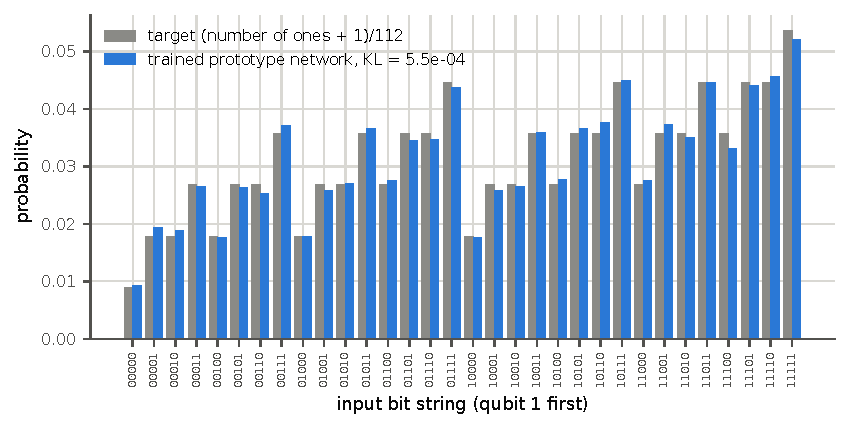
\includegraphics[width=\columnwidth]{fig_bitcount_histograms}
\caption{Target histogram (grey) and the trained prototype network's model distribution
(blue) over the 32 input strings; $\KL=5.5\times10^{-4}$.  Run
\run{bitcount\_noise/20260820T145335Z}, seed 1.}
\label{fig:agentic-histograms}
\end{figure}

\begin{figure}[tb]
\centering
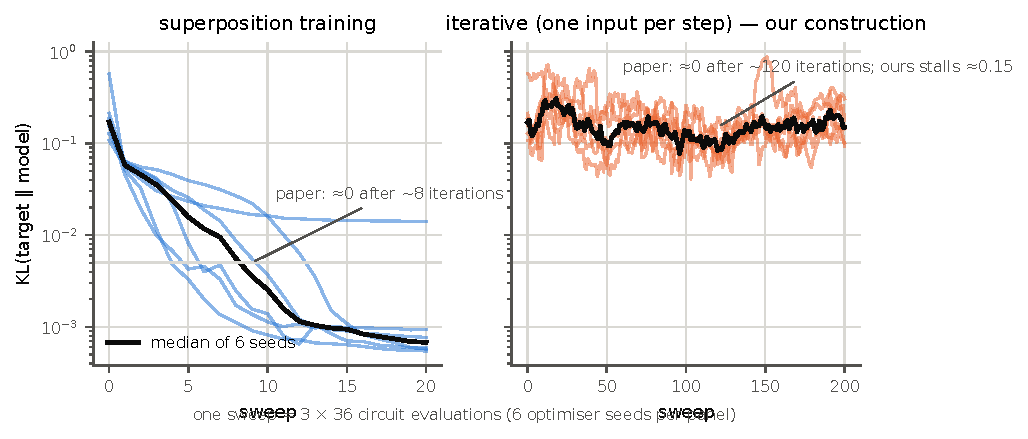
\includegraphics[width=\columnwidth]{fig_bitcount_convergence}
\caption{Left: superposition training, six optimiser seeds and their median.  Right: the
reimplementation's construction of the iterative baseline, which does not reach the
published curve.  Run \run{bitcount/20260820T135930Z}.}
\label{fig:agentic-convergence}
\end{figure}

\subsection{Iris}
\label{app:iris}

How the label enters the amplitude is not stated.  The published bar heights --- $1/86$, $4/86$,
$9/86$ on the training set and $1/154$, $4/154$, $9/154$ on the test set, two independent
integer normalisations --- fix the weight of class $\ell$ as $\propto(\ell+1)^2$: the amplitude
carries $\ell+1$ and the histogram its square, and no other exponent produces both
normalisations.  The split is not stated either; a stratified one-third training split
(50 flowers) is used.  Each feature is quantised into three $k$-means clusters, giving a 12-bit
one-hot code per flower, and the training set is loaded as one superposition over its distinct
codes; the network has 12 inputs, 4 hidden neurons and one output (17 qubits), against a
classic-neuron network of the same size, with labels predicted by rounding each code's read-out
weight.

In \cref{fig:agentic-iris-losses} the classic network drives its training loss to $10^{-5}$
within a few sweeps while its test loss bottoms out early and stays at $0.03$--$0.04$ --- it
memorises --- whereas the prototype network descends more slowly on both and its test loss is
still falling at sweep~40.  Prototype test accuracy is $95\,\%$, $91\,\%$ and $98\,\%$ on the
three splits against the published $\approx98\,\%$; the encoding caps accuracy at $97\,\%$,
$99\,\%$ and $99\,\%$, since two flowers of different species can share a 12-bit code.  The
t-SNE picture of \cref{fig:tsne} does not reproduce: in this embedding both weight sets cluster
away from the data, and what was plotted is not recoverable from the text.

\paragraph{On the split.}
The published histograms show 15 non-empty bars for the training set and 30 for the test set.
The 50-flower training splits used here give 14, 12 and 14 distinct codes, close to 15, but the
100-flower test splits give only 20, 20 and 18, not 30: three clusters per feature do not
spread 100 flowers over 30 codes on any split tried.  The figure supports the \emph{direction}
of the split, not its ratio, which remains an assumption.  An earlier draft claimed the bar
counts justified the ratio; an independent review caught the over-reading and the justification
was withdrawn.

\begin{figure}[tb]
\centering
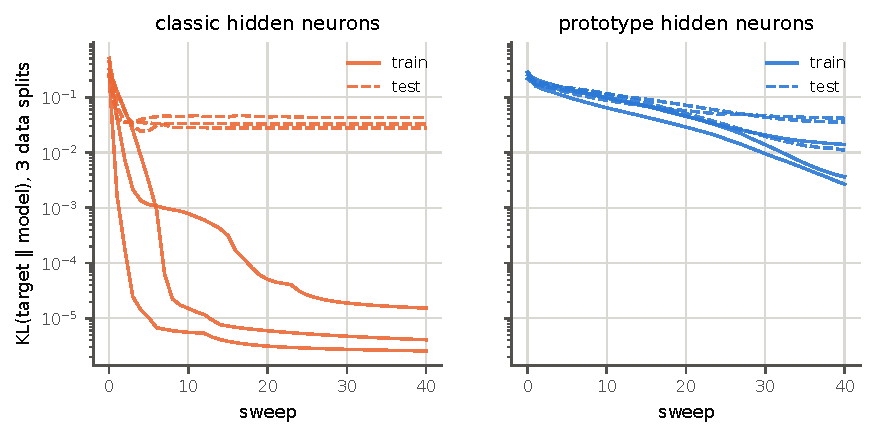
\includegraphics[width=\columnwidth]{fig_iris_losses}
\caption{Training (solid) and test (dashed) loss per sweep on three data splits, classic
against prototype network.  Runs \run{iris/20260820T144849Z}, \run{...T145454Z},
\run{...T145455Z}.}
\label{fig:agentic-iris-losses}
\end{figure}

\subsection{Flappy Bird}
\label{app:flappy}

The submission gives no reward, no training protocol and no game constants, so a
deterministic, window-free clone was built.  Its physics are a choice: the classic constants
(impulse $-9$, gap 100, spacing 144) are provably unplayable by a memoryless two-feature policy
--- one flap overshoots by 40.5\,px against a 38\,px budget --- so impulse $-7$, gap 120,
spacing 180 are used.  Height and the centre of the next gap enter two input qubits by
\cref{eq:agentic-encoding}; four prototype hidden neurons and one classic output flap when
$\Pout>\tfrac12$, 17 angles in all.  Training minimises the negative episode return (0.01 per
frame, 1 per pipe) plus a tracking term $|{\rm height}-{\rm gap}|$ supplying a slope where
every policy dies within 30 frames; 300 random vectors are scored on short episodes and the
best seeds 25 sweeps on five 1500-frame episodes.

The trained network passes 110 pipes in 5\,000 frames --- the cap, a perfect game --- on
all 20 held-out game seeds, for all 8 optimiser seeds tried, in about three minutes of training
(run \run{flappy/20260820T143753Z}); \cref{fig:agentic-flappy-policy} shows the learned
boundary.

\begin{figure}[tb]
\centering
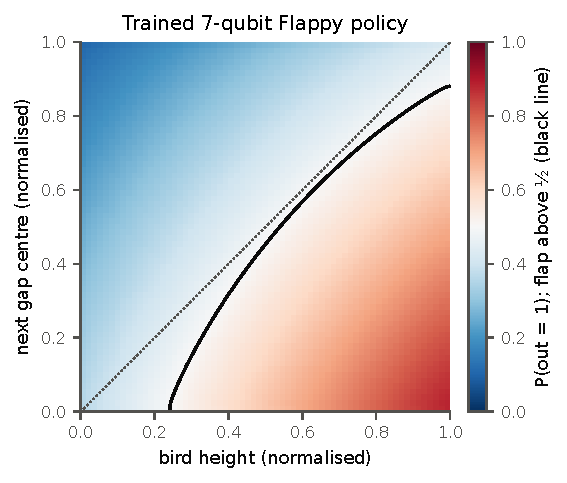
\includegraphics[width=0.85\columnwidth]{fig_flappy_policy}
\caption{The trained controller's activation $\Pout$ over the two observations; the black
line is the decision boundary $\Pout=\tfrac12$ (flap to its right), the dotted diagonal is
``bird at gap height''.  Run \run{flappy/20260820T143753Z}.}
\label{fig:agentic-flappy-policy}
\end{figure}

\subsection{ECG denoising}
\label{app:ecg}

Five consecutive noisy samples enter five input qubits; one to three prototype hidden neurons
and one output predict the clean centre sample as $\Pout$.  The recording is not identified;
the published trace is a smooth two-beat signal of 1\,800 samples in $[0,1]$ with additive
noise of standard deviation $\approx0.03$.  A synthetic ECG of McSharry form was generated to
match it, Gaussian noise of $\sigma=0.02$ added (noisy input $32.0$~dB), the first half used
for training and the second for test, and the experiment repeated on PhysioNet MIT-BIH
record~100~\cite{moody2001mitbih}.

PSNR is $37.4$, $38.0$ and $38.1$~dB for one, two and three prototype neurons against the
published $32.9$, $40.00$ and $40.04$: within about $2$~dB at two and three neurons, and $4$~dB
\emph{above} the published value at one neuron (\cref{fig:agentic-ecg-trace}).  The prototype
network beats the classic one at one and two neurons and on every SSIM; the classic one wins at
three.  The numbers cannot match exactly because the signal is not the authors' own.  The
alternative encoding $\theta=\pi s$ costs $0.6$--$7$~dB here, independent evidence for
\cref{eq:agentic-encoding}.  On MIT-BIH record~100 (run \run{ecg/20260820T165912}) the same
networks reach $36$--$38$~dB.

\begin{figure}[tb]
\centering
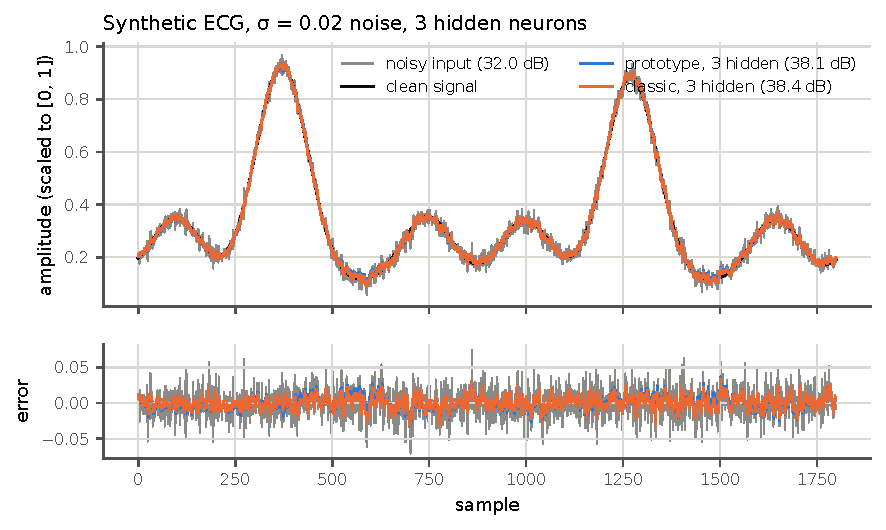
\includegraphics[width=\columnwidth]{fig_ecg_trace}
\caption{Noisy input, clean signal and the two three-neuron networks' outputs (top); their
errors (bottom).  Run \run{ecg/20260820T162014}.}
\label{fig:agentic-ecg-trace}
\end{figure}


\section{The experiments under calibrated noise}
\label{app:noise}

\subsection{Seven machines as noise models}
\label{app:devices}

Each vendor's published gate errors, gate durations, $T_1$, $T_2$, readout error and
connectivity were collected into a device file whose every field carries its source URL,
retrieval date (20 August 2026) and a verbatim quotation (\cref{app:provenance});
\cref{tab:agentic-devices} summarises them.  Three caveats govern everything that follows.
\emph{Quantinuum publishes no gate durations and no $T_1$/$T_2$}: its idle error is charged
from its published memory error per depth-1 circuit time ($2.0\times10^{-4}$ for H2-1,
$2.2\times10^{-4}$ for H1-1), and its simulated noise carries no idle error.  \emph{Rigetti
publishes only a two-qubit error} for Ankaa-3, its $99.5\,\%$ headline being for a different
gate than the universal one needed here, so every Rigetti number is an upper bound.
\emph{IQM's $T_1$/$T_2$ are a third-party snapshot}, and its $T_2$ without echo is $8.5\,\mu$s
against the $21\,\mu$s echo value used.  Where a vendor publishes nothing, the channel is
modelled as error-free and flagged, not invented.

\begin{table*}[t]
\caption{The seven device presets (medians where the vendor publishes per-qubit tables).
Two-qubit error $\varepsilon_2$, one-qubit error $\varepsilon_1$, readout error (mean of
$p_{01}$, $p_{10}$), coherence times, two-qubit gate time.  ``---'' = not published.}
\label{tab:agentic-devices}
\begin{tabular}{@{}l l S[table-format=1.2e-1] S[table-format=1.1e-1] S[table-format=1.1e-1] l l S[table-format=6.0]@{}}
\toprule
Machine & Connectivity & {$\varepsilon_2$} & {$\varepsilon_1$} & {readout} & $T_1$ & $T_2$ & {2q gate (ns)} \\
\midrule
Quantinuum H1-1 & all-to-all & 9.7e-4 & 1.8e-5 & 2.3e-3 & --- & --- & {---} \\
Quantinuum H2-1 & all-to-all & 1.1e-3 & 1.9e-5 & 1.0e-3 & --- & --- & {---} \\
IonQ Forte & all-to-all & 4.0e-3 & 2.0e-4 & 5.0e-3 & 55\,s & 1\,s & 950000 \\
Google Willow & square & 4.1e-3 & 5.3e-4 & 8.0e-3 & $68\,\mu$s & $89\,\mu$s & 42 \\
IBM Fez (Heron r2) & heavy-hex & 3.9e-3 & 2.3e-4 & 7.7e-3 & $145\,\mu$s & $88\,\mu$s & 84 \\
IQM Garnet & square & 4.9e-3 & 8.0e-4 & 3.0e-2 & $27\,\mu$s & $21\,\mu$s & 30 \\
Rigetti Ankaa-3 & square & 1.0e-2 & {---} & {---} & --- & --- & 72 \\
\bottomrule
\end{tabular}
\end{table*}

\subsection{Bit-count}
\label{app:noise-bitcount}

The trained 11-qubit networks were evaluated exactly, as density matrices on the GPU, under
each preset (run \run{bitcount\_noise/20260820T145335Z};
\cref{fig:agentic-noise-devices}).  The model distribution moves by $\TV=0.005$ (Quantinuum
H2-1) to $0.039$ (IQM Garnet), and the KL to the target rises from $5.5\times10^{-4}$ to
$7\times10^{-4}$ on H2-1 and to $6\times10^{-3}$ on Garnet.  The prototype network is better
under every preset, but the displacement \emph{caused} by the noise,
$\KL(\text{clean}\,\|\,\text{noisy})$, is the same for both (median $0.0021$ against $0.0022$):
they have identical two-qubit gate counts, so the prototype's advantage under noise is
inherited from its better noiseless fit, not from robustness of the neuron type.  Scaling IBM
Fez's noise by $s$ gives $\KL\propto s^{1.7}$ and $\TV\propto s^{0.95}$.

Training \emph{under} the noise works, on a 7-qubit version (3 inputs, 3 hidden; the 11-qubit
grid would have cost 13 hours and was not run): it recovers the noisy KL by a median factor of
$158$ (prototype) and $361$ (classic), \cref{fig:agentic-noise-aware}.  But the recovered
parameters are \emph{worse} on a noiseless simulator --- the optimiser folds the channel into
the angles instead of finding noise-robust ones.

\begin{figure}[tb]
\centering
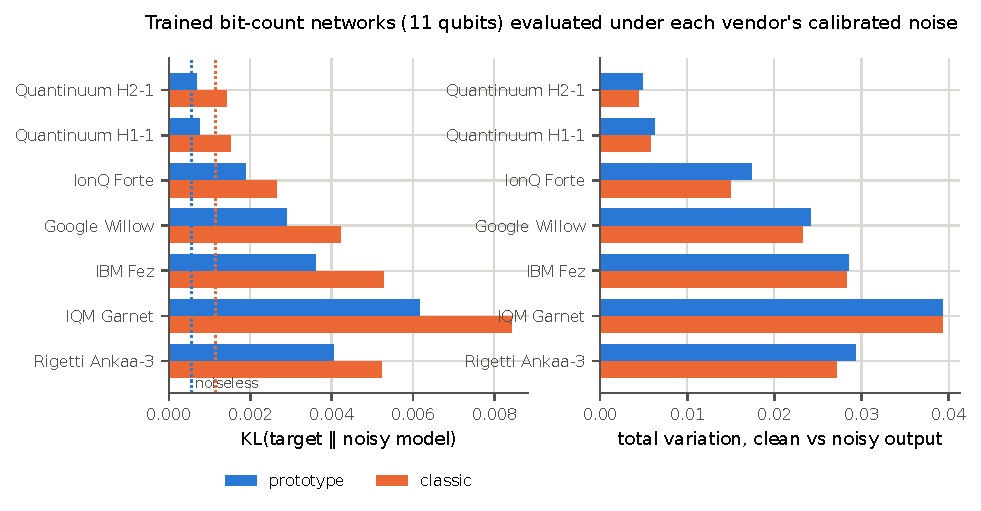
\includegraphics[width=\columnwidth]{fig_bitcount_noise_devices}
\caption{The trained bit-count networks under each machine's noise model.  Left: KL to the
target, noiseless values dotted.  Right: how far the output distribution moved.  Rigetti's
row models only its two-qubit error.  Run \run{bitcount\_noise/20260820T145335Z}.}
\label{fig:agentic-noise-devices}
\end{figure}

\begin{figure}[tb]
\centering
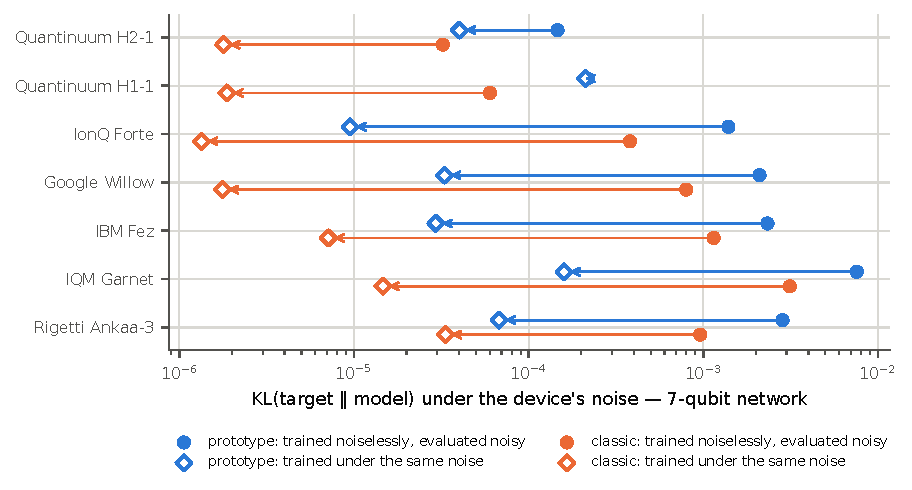
\includegraphics[width=\columnwidth]{fig_bitcount_noise_aware}
\caption{Noise-aware training of the 7-qubit bit-count network: KL under each machine's noise
for parameters trained noiselessly (filled) and with the same noise model in the loop (open),
median of three seeds.  Same run.}
\label{fig:agentic-noise-aware}
\end{figure}

\subsection{Flappy Bird}
\label{app:noise-flappy}

For a thresholded activation what matters is not how far $\Pout$ moves but whether it crosses
$\tfrac12$.  Evaluated exactly under every preset on its $65\times65$ decision grid and played
for 20 held-out games (run \run{flappy\_noise/20260820T154249Z};
\cref{fig:agentic-flappy-noise}), the controller \emph{still plays perfectly on all seven
machines}: only $1.5$--$4\,\%$ of visited frames are decided differently, because the noise
contracts every activation toward $\tfrac12$ by about the same amount (mean
$|\Delta P|=0.002$--$0.018$) and so rarely changes the ordering.  There is a factor of two of
headroom: Fez's noise scaled by $2$ leaves $60\,\%$ of games perfect, by $4$ none.

Shot noise is a different matter (\cref{fig:agentic-flappy-shot-noise}).  Re-deciding every
frame from $N$ measurements, the controller wins no game at $N=1\,000$, $90\,\%$ at $4\,000$
and all at $10\,000$ noiselessly; on Fez's model only $55\,\%$ at $4\,000$.  The cause is the
margin distribution over played frames: median $\delta=0.019$, tenth percentile $0.004$, first
percentile $0.0002$; the measured flip rate agrees with the average of $\Phi(-2\delta\sqrt N)$
over it to $3\,\%$.  A deterministic shift of the boundary is tolerated far past a stochastic
one --- Fez at scale $2$ decides $20\,\%$ of frames differently and still wins $60\,\%$ of
games, while $1\,000$ shots decide only $8.5\,\%$ differently and win none ---.  Fine-tuning under Fez's noise for five sweeps changes nothing: the training
episodes all survive already, so the objective has no slope.

\begin{figure}[tb]
\centering
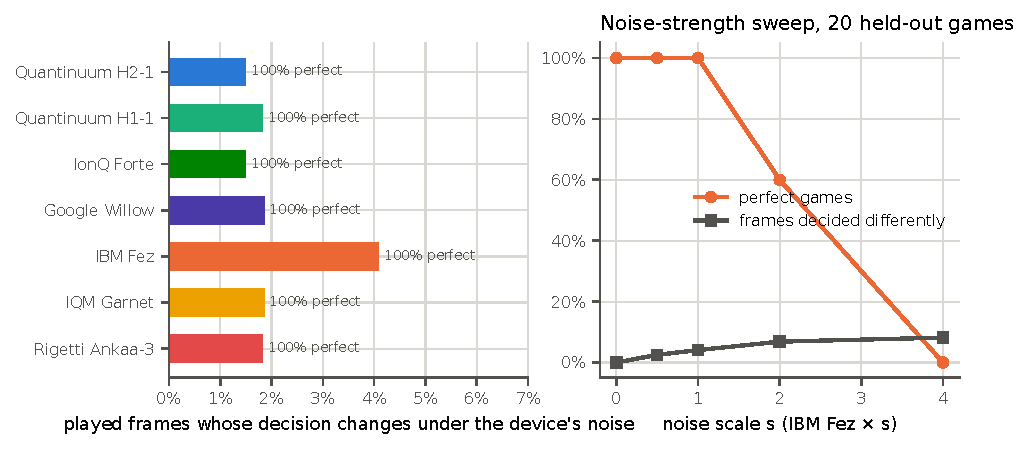
\includegraphics[width=\columnwidth]{fig_flappy_noise}
\caption{Flappy under gate noise.  Left: fraction of played frames whose decision changes
under each machine's model; every machine still yields $100\,\%$ perfect games.  Right: IBM
Fez's noise scaled by $s$.  Run \run{flappy\_noise/20260820T154249Z}.}
\label{fig:agentic-flappy-noise}
\end{figure}

\begin{figure}[tb]
\centering
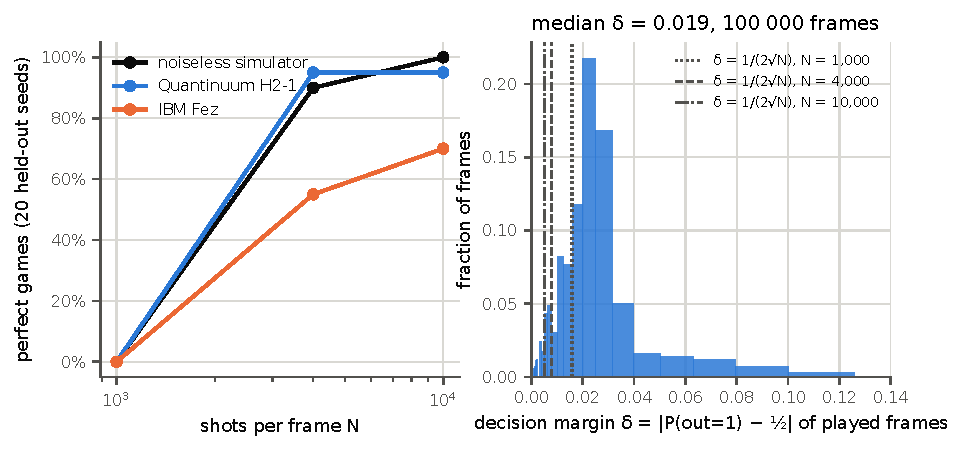
\includegraphics[width=\columnwidth]{fig_flappy_shot_noise}
\caption{Flappy under shot noise.  Left: perfect games when every frame is decided from $N$
shots.  Right: distribution of the decision margin $\delta$ over the $100\,000$ frames the
noiseless controller plays; vertical lines mark the margin that $N$ shots can just resolve.
Same run.}
\label{fig:agentic-flappy-shot-noise}
\end{figure}

\subsection{ECG and Iris, reduced run}
\label{app:noise-ecg-iris}

These two grids were run in a \emph{reduced} configuration only (run
\run{ecg\_iris\_noise/20260820T155618Z}): ECG on 8 test windows instead of 898 and two presets
instead of seven; Iris with 16 Monte-Carlo trajectories per evaluation instead of 2\,000
(per-outcome standard error $\approx12\,\%$), two presets, and perfect preparation of the
dataset state assumed.  The full grids cost 4--6 CPU-hours (ECG) and 8 hours (Iris), outside
the budget.  The results (\cref{fig:agentic-ecg-iris-noise}) are indicative only: ECG loses
$-0.1$ to $+0.4$~dB under Quantinuum H2-1 and $1.6$--$2.7$~dB (classic) under IBM Fez, while
the prototype cells \emph{gain} up to $3.8$~dB under Fez on eight windows --- a small-sample
artefact, not a finding.  Iris keeps its $95\,\%$ accuracy under H2-1 and loses it under Fez
($64\pm44\,\%$ over two trajectory seeds) for the prototype network, whose read-out is a
conditional distribution over 4\,096 input strings and is therefore directly exposed to
probability leaking out of the 20-code support.  One noisy sweep of ECG fine-tuning gains
$2.7$~dB under Fez and $3.7$~dB noiselessly: it finishes the clean optimisation, it does not
fold the channel in.

\begin{figure}[tb]
\centering
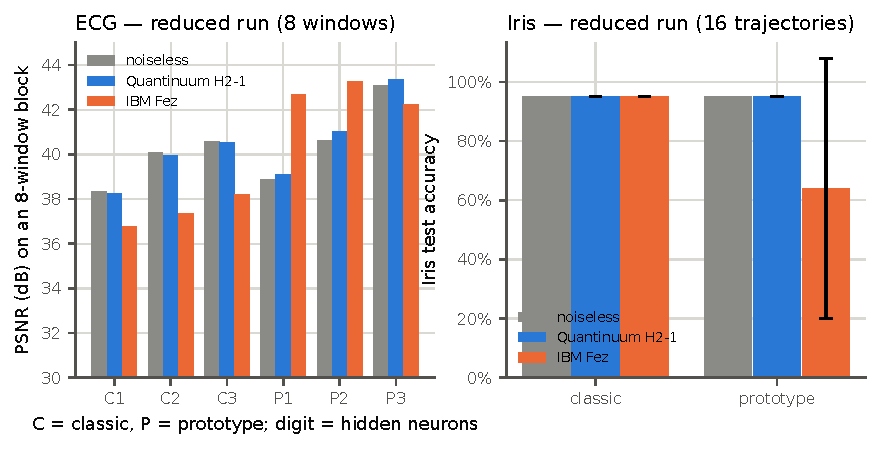
\includegraphics[width=\columnwidth]{fig_ecg_iris_noise}
\caption{Reduced-configuration noise runs, quoted for the record.  Left: ECG PSNR on an
8-window block.  Right: Iris test accuracy from 16 trajectories, error bars over two
trajectory seeds.  Run \run{ecg\_iris\_noise/20260820T155618Z}.}
\label{fig:agentic-ecg-iris-noise}
\end{figure}


\section{What it takes to run this on a real machine}
\label{app:hardware}

All numbers here are printed by one script into \run{hardware-plan/20260821T084554Z} (file
\code{numbers.md}); it joins every calibration number to its provenance entry and refuses to
run if one is missing.

\subsection{Compilation}
\label{app:compile}

Every prototype neuron touches every input, so the two-qubit gates form a complete bipartite
graph between inputs and hidden qubits --- the worst case for a lattice.  On an all-to-all
machine each controlled rotation costs exactly two native two-qubit gates: 24 for Flappy, 60
for bit-count.  On a lattice the compiler must insert SWAPs at three native gates each; with a
greedy router the bit-count circuit needs 327 native two-qubit gates on IBM's heavy-hex lattice
and 207 on a square lattice, $82\,\%$ and $71\,\%$ of them SWAP-borne
(\cref{fig:agentic-entanglers}).  IBM's own compiler needs 97 at optimisation level~2,
$3.4\times$ fewer, so this router is a device-independent comparison instrument and not what
one would submit.  The Flappy circuit is $12.9\,\mu$s long on Fez ($1.56\,\mu$s of it readout)
and 17.9\,ms on IonQ Forte, whose gates take a millisecond.

\begin{figure}[tb]
\centering
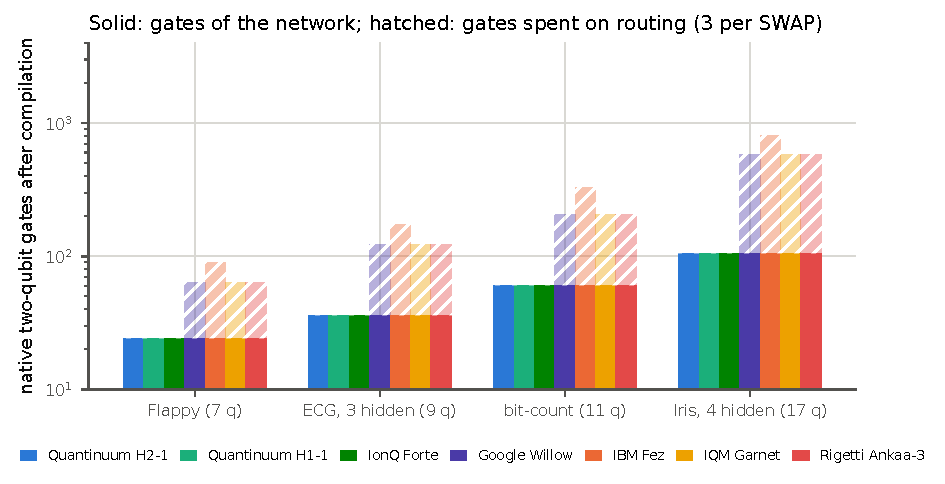
\includegraphics[width=\columnwidth]{fig_hardware_entanglers}
\caption{Native two-qubit gates after compiling each network for each machine (greedy router,
log scale).  All-to-all machines need only the network's own gates; the lattices spend most of
their budget on routing.  Run \run{hardware-plan/20260821T084554Z}.}
\label{fig:agentic-entanglers}
\end{figure}

\subsection{Expected fidelity}
\label{app:fidelity}

\Cref{fig:agentic-fidelity} stacks the four factors of \cref{eq:agentic-fidelity} for the two
smallest circuits, with the exactly simulated total-variation distance between the compiled
circuit run clean and run under noise beside each bar.  Flappy at 7 qubits is a high-fidelity
circuit on trapped ions ($F\approx0.92$ on H2-1, $0.83$ on Forte), marginal on Willow and Fez
($0.63$; $0.46$ with the greedy router, $0.75$ with IBM's compiler) and poor on Garnet
($0.24$).  Bit-count at 11 qubits is feasible on the H-series ($0.81$) and Forte ($0.64$),
usable with IBM's compiler on Fez ($0.48$) and dead on Garnet ($0.008$), whose routed circuit
lasts $86\,\%$ of its $T_2$.  Idling is charged only over each qubit's schedule gaps, since
relaxation during a gate is already inside the vendor's gate error; charging the whole circuit
duration on every qubit is $10$--$15$ points more pessimistic on the superconducting machines
and is printed beside it in the run directory.

Two cautions.  The simulated distances of the \emph{compiled} circuits ($0.03$ on the H-series,
$0.16$ on Forte, $0.43$ on Fez) are $5$--$15\times$ larger than for the uncompiled circuits of
\cref{app:noise-bitcount}.  And vendors' two-qubit errors are measured in isolation --- IBM's
own layered benchmark for Fez is $1.7\times$ worse than its isolated gate error --- so the
lattice numbers are optimistic.

\begin{figure*}[t]
\centering
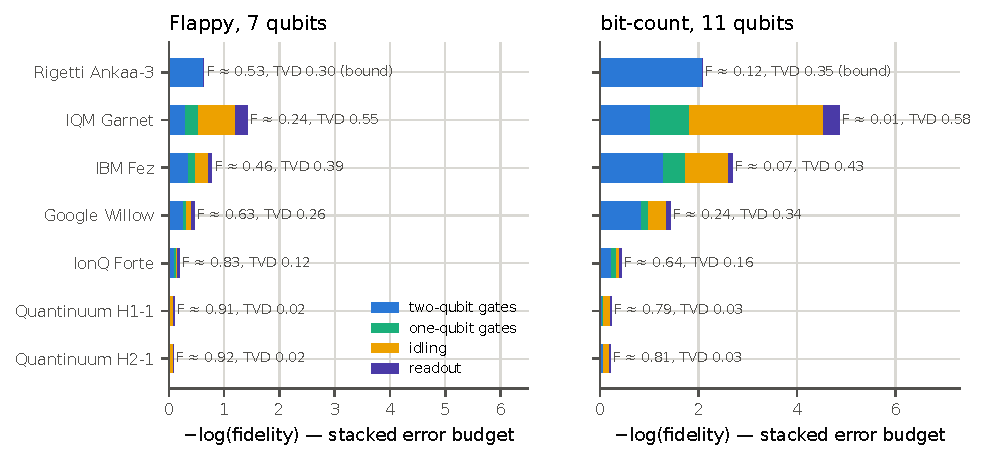
\includegraphics[width=0.92\textwidth]{fig_hardware_fidelity}
\caption{Error budget per machine for the Flappy (left) and bit-count (right) circuits: the
stacked bars are $-\log$ of each factor of \cref{eq:agentic-fidelity}, so their total is
$-\log F$; labels give $F$ and the simulated total-variation distance of the compiled circuit.
Quantinuum's idle term comes from its published memory error; Rigetti's is a bound from its
two-qubit error only.}
\label{fig:agentic-fidelity}
\end{figure*}

\subsection{Shots, time and money}
\label{app:cost}

An activation to $\pm0.005$ needs $10\,000$ shots.  The 32-bin bit-count histogram is estimated
from the shots in which the output fired ($\Pout=0.487$ of them), so the plug-in KL is biased
upward by $(K-1)/(2\cdot0.487\cdot N)=31.8/N$ with $K=32$; reaching the trained model's
$5.5\times10^{-4}$ needs $58\,000$ shots, rounded to a $64\,000$-shot job.  The ECG PSNR is
capped by shot noise at $10\log_{10}(4N)$, so $2\,500$ shots per sample cap it at exactly
$40$~dB --- the published Table~I value --- and a $1\,800$-sample trace at $25\,000$ shots is
$4.5\times10^7$ shots: ECG is a simulator experiment.  Machine time per job is milliseconds to
two seconds on the superconducting machines, where the per-job overhead dominates, but $72$\,s
(Flappy) and 32 minutes (bit-count) on IonQ Forte, where circuit time does.

Prices retrieved 20 August 2026 are in \cref{tab:agentic-cost}.  Training on hardware is out of
the question: $2\,160$ evaluations at $64\,000$ shots are $1.4\times10^8$ shots, 48 days of
Forte time or \$11\,M.  Fine-tuning the six output angles (90 evaluations at $4\,000$ shots) is
$1.8$ hours on Forte, about 45 minutes on Fez.  Live play is equally out: $1\,500$ frames
$\times$ $4\,000$ shots $\times$ $17.9$\,ms is 30 hours per episode on Forte.  The falsifiable
hardware observable is instead the activation map of \cref{fig:agentic-flappy-policy} on a grid
of observations, 16 jobs.

\begin{table*}[t]
\caption{Cost per job (file \code{numbers.md}, section ``cost'').  IBM: \$1.60 per QPU second
plus a 30\,s per-job overhead, both assumptions (\cref{app:assumptions}); Quantinuum: the
vendor's credit formula converted at the Azure plan rate; Braket: published per-shot prices.}
\label{tab:agentic-cost}
\begin{tabularx}{\textwidth}{@{}l X l l@{}}
\toprule
Machine & Price model & Flappy, 4\,000 shots & bit-count, 64\,000 shots \\
\midrule
IBM Fez & \$1.60/s; 52\,ms resp.\ 1.8\,s of QPU & \$0.08 (\$48 with overhead) & \$2.85 (\$51) \\
IBM Open plan & 10 min per 28 days, free & \$0 & \$0 \\
Quantinuum H1/H2 & credits $=5+(N_1+10N_2+5N_m)C/5000$ & 323 credits $\approx$ \$4\,030 & 11\,920 credits $\approx$ \$149\,000 \\
IonQ Forte (Braket) & \$0.30 + \$0.08/shot & \$320 & \$5\,120 \\
IQM Garnet (Braket) & \$0.30 + \$0.00145/shot & \$6.10 & \$93 \\
\bottomrule
\end{tabularx}
\end{table*}

\subsection{Recommendation}
\label{app:recommendation}

Run the 7-qubit Flappy activation map first: on IBM's free plan to debug the pipeline (readout
calibration, then zero-noise extrapolation by gate folding, both validated offline against the
noise model), then on IonQ Forte for the confirmation (\$1\,300 for a $4\times4$ grid at
$1\,000$ shots), and on Quantinuum H2-1 for the headline number if an allocation exists.  The
bit-count histogram is feasible on the H-series and Forte as a \emph{shape} demonstration but
not as a KL comparison: device error puts the KL floor at $10^{-2}$--$10^{-1}$, two orders
above the simulated $5.5\times10^{-4}$.  Iris cannot be settled yet.  What these runs prepare
is a uniform superposition over the $12$--$14$ \emph{distinct} training codes, not over the 120
samples an earlier draft assumed; the sparse state-preparation construction of Gleinig and
Hoefler~\cite{gleinig2021sparse} has leading term $k\cdot n=144$--$168$ two-qubit gates, giving
$F\approx0.83$ on H2-1 and $\approx0.75$ with the network --- but its constant is unknown, and
the dense alternatives ($8\,168$ gates by Shende--Bullock--Markov synthesis, $\approx3\,925$ by
Plesch--Brukner) are hopeless.  An exact answer needs an actual sparse state-preparation
circuit, which the repository does not build.  For a live submission the code still lacks
credentials, the vendors' own routing, asynchronous job handles, and readout-unfolding and
gate-folding utilities.


\section{The shot-noise programme}
\label{app:shots}

What limits a hardware demonstration is the number of measurements, through two mechanisms: a
thresholded controller flips at a rate $\Phi(-2\delta\sqrt N)$, and a histogram loss estimated
from $N$ shots is biased upward by $(K-1)/(2\,\Pout\,N)$ while discarding the half of the shots
in which the output did not fire.  Six remedies were proposed and three implemented.  The
others --- a joint-distribution loss or amplitude amplification so that all shots are used,
bias-corrected KL estimators, and amplitude estimation --- are designed but not implemented;
the first is the natural next step, since the estimator bias is what now limits sampled
training.  All runs here are noiseless state-vector simulations plus sampling.

\subsection{Margin-aware training: negative}
\label{app:margin}

If every frame had $\delta\ge0.1$ instead of the median $0.019$, the shots per frame would fall
by $(0.1/0.019)^2\approx25\times$ at no noiseless cost.  A penalty
$w\times0.01\times\max(0,1-\delta/m)$ per played frame was added --- a fraction $w<1$ of the
$0.01$ reward for surviving that frame, so surviving always beats dying confidently --- and the
controller fine-tuned for 25 sweeps with $m=0.1$, $w\in\{0.25,0.5,1\}$ (run
\run{flappy\_shots/20260821T084601Z}).  An earlier attempt with a \emph{mean} hinge of weight
20, trained from scratch, collapsed to a policy that died in 30 frames with perfectly confident
decisions (run \run{flappy\_shots/20260821T075048Z}): any penalty that can outweigh the
per-frame reward selects for dying early.

The margin quantiles hardly move (\cref{fig:agentic-flappy-shots}, left; median
$0.019\to0.021$--$0.024$, tenth percentile $0.004\to0.006$).  All three fine-tuned controllers
still play perfectly on exact probabilities, but under shot noise they play \emph{worse} than
the original at $w\ge0.5$ ($50\,\%$ and $80\,\%$ perfect games at $10\,000$ shots against
$100\,\%$).  The near-boundary frames are those in which the bird hovers at the boundary, a
property of the game's dynamics and not of the surface's steepness, so penalising them moves
the boundary rather than steepening it --- and a 17-parameter network has no spare capacity to
steepen its surface anyway.

\subsection{Common random numbers}
\label{app:crn}

A slope from $N$ independent shots per probe with variance $\sigma^2$ has variance
$\sigma^2/2c^2$, at $c=0.2$ some $12.5\sigma^2$, which is why finite differences on a sampling
backend stall.  Feeding the same uniform random numbers to both probes gives only a
$1.3\times$ reduction, because a parameter change moves probability between distant bit strings
and shifts every later bin boundary.  What works is the \emph{maximal coupling}: sample the
first probe, then for the second keep each outcome $i$ with probability
$\min(1,p_{\mathrm{new}}(i)/p_{\mathrm{ref}}(i))$ and redraw otherwise from
$(p_{\mathrm{new}}-p_{\mathrm{ref}})_+$.  The second sample has exactly the right distribution
and only $N\cdot\TV(p_{\mathrm{new}},p_{\mathrm{ref}})$ shots change; since $\TV\propto c$, the
slope's variance is $O(1/(cN))$ rather than $O(1/(c^2N))$, a gain of order $1/c$.  Coupling
reduces the variance of the slope, not the bias of a non-linear loss.  On hardware the analogue
is to interleave the $\pm c$ circuits in one job so they share the same drift.

Measured on one slope of the bit-count loss at 400 shots per probe, the reduction is
$\times2$--$3$ at $c=0.2$--$0.4$ and $\times22$--$29$ at $c=0.025$--$0.05$, both estimates
unbiased for the exact slope.  Training the 11-qubit network on a sampling backend (run
\run{bitcount\_shots/20260821T084558Z}) gives, after 20 sweeps, an exact KL improving from
$0.080$ to $0.059$ at $N=1\,000$ shots per evaluation, from $0.050$ to $0.014$ at $4\,000$, and
at $16\,000$ the two are within the seed-to-seed spread ($0.029$ against $0.033$) --- all an
order of magnitude above the exact-probability result ($0.0009$).  The likely reason is the
loss itself: a plug-in KL of a 32-bin histogram from about $N/2$ usable shots, biased by
$31.8/N$, with the reached KL tracking one to three times that bias.  Three seeds, one of which
stalls at $0.014$ even on exact probabilities, cannot separate estimator from optimiser; a
bias-corrected or joint loss under paired initialisations is the test, and it has not been run.
The schedule used ($c_0=0.2$ decaying only to $0.15$ over 20 sweeps) also keeps the optimiser
where the reduction is smallest.

\subsection{Sequential decisions: positive}
\label{app:sprt}

A fixed budget wastes most of its shots: a frame with $\delta=0.3$ is decided correctly after a
dozen.  Wald's sequential probability ratio test~\cite{wald1945} between
$\Pout=\tfrac12\pm\delta_0$ draws shots in blocks, computes after $n$ shots with $k$ ones the
log-likelihood ratio $\Lambda=(2k-n)\log\frac{1+2\delta_0}{1-2\delta_0}$, and stops when
$\Lambda\ge\log\frac{1-\beta}{\alpha}$ (flap) or $\Lambda\le\log\frac{\beta}{1-\alpha}$ (do
not), up to a cap after which the majority decides.  Beyond $\delta_0$ its error probability is
at most about $\alpha$ ($=\beta=5\,\%$ here); nearer the boundary it is slow and unbounded.

On the same 20 held-out games (\cref{fig:agentic-flappy-shots}; \cref{tab:agentic-sprt}) the
rule with $\delta_0=0.01$ and cap $10\,000$ wins \emph{every} game at a mean of $2\,191$ shots
per frame, against the $10\,000$ a fixed budget needs for the same result --- $4.6\times$ fewer
--- and with $\delta_0=0.005$, cap $4\,000$ it matches the fixed $4\,000$-shot result
($85\,\%$) at $2\,916$.  Setting $\delta_0$ at the median margin ($0.02$) fails ($30\,\%$
perfect at $822$ shots): the frames that decide a game are the near-boundary ones, so the
indifference margin must sit below \emph{their} margins, the tenth percentile of
$0.004$--$0.006$.  The rule needs no change to the network and no retraining.

\begin{figure*}[t]
\centering
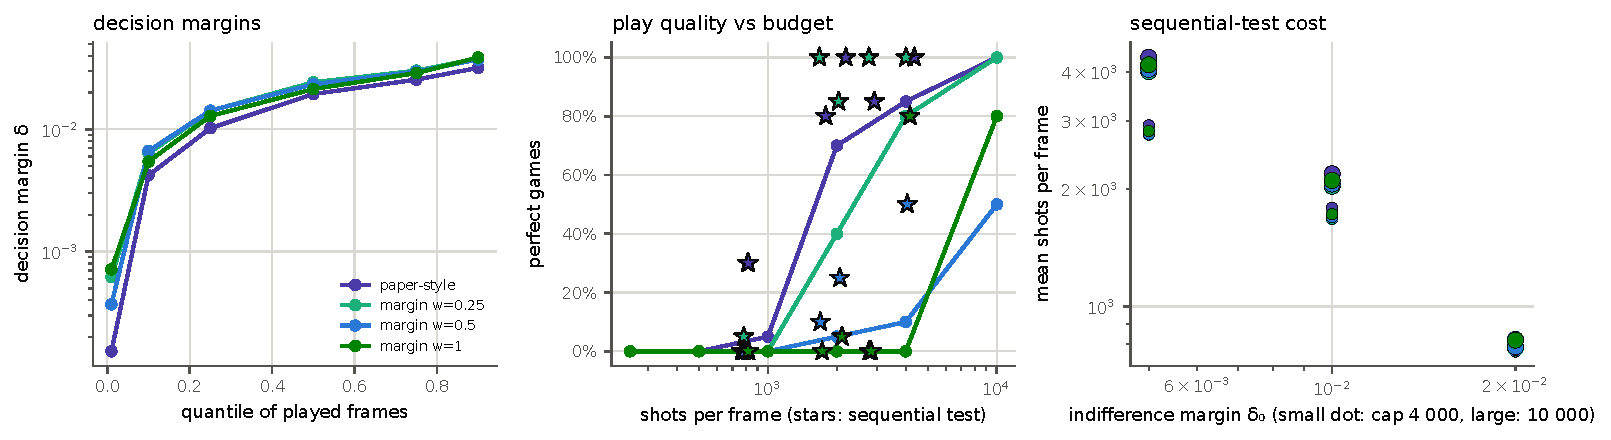
\includegraphics[width=\textwidth]{fig_flappy_shots_programme}
\caption{Flappy under shot noise, remedies 1 and 3.  Left: decision-margin quantiles of the
frames played by the original and the three margin-aware controllers.  Middle: perfect games
against shots per frame for a fixed budget (lines) and for the sequential test (stars, plotted
at the mean number of shots it actually spent).  Right: mean shots per frame of the sequential
test against its indifference margin $\delta_0$.  Run
\run{flappy\_shots/20260821T084601Z}.}
\label{fig:agentic-flappy-shots}
\end{figure*}

\begin{table*}[t]
\caption{Flappy, original controller, 20 held-out games: fixed shot budgets against the
sequential test ($\alpha=\beta=0.05$, blocks of 20 shots).  ``Flips'' are frames decided
differently from the exact rule.  Run \run{flappy\_shots/20260821T084601Z}.}
\label{tab:agentic-sprt}
\begin{tabular}{@{}l S[table-format=3.0] S[table-format=3.0] S[table-format=2.2] S[table-format=5.0]@{}}
\toprule
Decision rule & {perfect games (\%)} & {median pipes} & {flips (\%)} & {mean shots/frame} \\
\midrule
fixed $N = 1\,000$ & 5 & 23 & 8.36 & 1000 \\
fixed $N = 2\,000$ & 70 & 110 & 7.40 & 2000 \\
fixed $N = 4\,000$ & 85 & 110 & 6.09 & 4000 \\
fixed $N = 10\,000$ & 100 & 110 & 4.47 & 10000 \\
sequential, $\delta_0 = 0.02$, cap $10\,000$ & 30 & 88 & 7.19 & 822 \\
sequential, $\delta_0 = 0.01$, cap $4\,000$ & 80 & 110 & 6.12 & 1790 \\
sequential, $\delta_0 = 0.005$, cap $4\,000$ & 85 & 110 & 5.98 & 2916 \\
sequential, $\delta_0 = 0.01$, cap $10\,000$ & 100 & 110 & 5.06 & 2191 \\
sequential, $\delta_0 = 0.005$, cap $10\,000$ & 100 & 110 & 4.50 & 4358 \\
\bottomrule
\end{tabular}
\end{table*}


\section{What the reproduction learned}
\label{app:learnings}

\begin{enumerate}
\item \textbf{The central claims reproduce.}  Activation surface, bit-count histogram and
convergence, Iris overfitting contrast, perfect Flappy play on a clone, ECG denoising within
2~dB on a different signal.  What does not: the iterative baseline of \cref{fig:OptConv} (this
construction stalls at $\KL\approx0.15$) and the weight picture of \cref{fig:tsne}; both are
under-specified in the text.

\item \textbf{Reading figures is part of reproduction.}  The bit-count target
$(\text{ones}+1)/112$, the Iris label weighting $(\ell+1)^2$ and the angle encoding
$\theta=2\arcsin\sqrt s$ were all read off figures and then confirmed to the figure's
precision.  Where a figure was over-read --- the Iris split ratio --- an independent review
caught it and the justification was withdrawn (\cref{app:iris}).

\item \textbf{The prototype network's advantage under noise is inherited, not intrinsic.}  Both
networks have the same two-qubit gate count and the noise displaces both equally; the prototype
wins under noise because it fits better without it.

\item \textbf{Gate noise at published levels is not the obstacle; shots are.}  Every
7--11-qubit network survives every vendor's calibrated model with a qualitatively intact
result, while the Flappy controller needs $10^4$ shots per frame at a fixed budget and the
bit-count loss is biased by $31.8/N$.  The one remedy that pays now is the sequential rule
($4.6\times$ fewer shots, no retraining); margin-aware training does not work for a
17-parameter network; common random numbers reduce the optimiser's noise by $1/c$ but leave the
estimator's bias, the likely and as yet untested limit of sampled training.

\item \textbf{Compiled circuits are $5$--$15\times$ more noise-sensitive than logical ones.}
Two native gates per controlled rotation, resynthesised single-qubit gates and lattice routing
all cost; a complete-bipartite network is the worst case for a lattice, so the vendor's own
compiler must be used for any superconducting submission.  Trapped ions are the natural home of
this architecture, at the price of circuit time.

\item \textbf{An optimiser that keeps a stale incumbent turns a harmless change into a negative
result.}  The ``rotating episodes break training'' finding was an artefact of comparing losses
measured on different episode batches, because the optimiser kept its incumbent's loss from the
previous batch; re-scoring the incumbent on each batch restores $25/25$ perfect games (runs
\run{flappy/batch0}, \run{flappy/batch5}).  Any non-stationary objective needs this.

\item \textbf{Penalties must be priced in the currency of the reward.}  A margin hinge able to
outweigh the per-frame survival reward produced a confidently dead controller; the per-frame
form, kept below that reward, does not.

\item \textbf{Provenance has to be mechanical.}  The first hardware plan contained a dozen wrong
numbers: a state-preparation gate count off by a factor of two, a reversed inequality, costs
computed by hand.  The fix was a script that emits every number and refuses to run if any
calibration input lacks a source; this appendix quotes only that script.
\end{enumerate}


\section{Choices the submission leaves open}
\label{app:assumptions}

Each entry is marked \code{[ASSUMPTION]} where it enters the code.

\begin{description}
\item[Optimiser schedule.]  $a_n=a_0/(n+1)^{0.602}$, $c_n=c_0/(n+1)^{0.101}$, geometric
cooling; one iteration is a coordinate sweep.  Bit-count: $a_0=20$, $c_0=0.2$, $T_0=0.02$,
cooling $0.7$, 20 sweeps.  Flappy: $a_0=0.4$, $c_0=0.25$, $T_0=0.05$, cooling $0.9$, 25 sweeps
after 300 random restarts.  Iris: $a_0=2$, decay exponent $0.3$, $c_0=0.1$, 40 sweeps.  ECG:
100 sweeps with restarts.
\item[Iterative baseline.]  One optimiser sweep on the squared error of one random input per
iteration.
\item[Angle encoding.]  $\theta=2\arcsin\sqrt s$, pinned by a printed angle in the companion
paper; $\theta=\pi s$ tested as an ablation.
\item[KL regularisation.]  Model probability floored at $10^{-12}$ inside the logarithm.
\item[Iris.]  Stratified one-third training split; flowers sharing a code are merged and their
labels averaged; the KL is normalised over all 4\,096 input strings, since restricting it to
the dataset's codes lets the network exploit interference between examples and reach a training
loss of $10^{-5}$ while reading out at chance; label weight $\propto(\ell+1)^2$; labels
predicted by nearest rounding of the read-out weight.
\item[Flappy.]  Clean-room clone: $288\times512$ screen, flap impulse $-7$, gap 120, pipe
spacing 180, gravity 1; reward 0.01 per frame plus 1 per pipe; tracking term
$|{\rm height}-{\rm gap}|$ with weight 1; 5 training episodes of 1\,500 frames, 20 held-out
seeds 5--24, 5\,000-frame cap (110 pipes); decisions cached on a $65\times65$ grid.
\item[ECG.]  Synthetic McSharry-form signal tuned to the published trace, and MIT-BIH
record 100; Gaussian noise $\sigma=0.02$; mirror-padded edges; first half train, second half
test; PSNR with $R$ the range of the clean signal; SSIM in a 7-sample sliding window.
\item[Noise model.]  Depolarising at the vendor's average gate error, relaxation during gates
and as-soon-as-possible idling, readout confusion; medians where vendors publish per-qubit
tables; no crosstalk, since no vendor publishes a usable number.  Quantinuum's idle error is
charged as $(1-m)^{n_{\rm qubits}\cdot{\rm depth}}$ from its memory error per depth-1 time;
IQM's and Rigetti's unpublished one-qubit gate durations are set to 40\,ns.
\item[Fidelity estimate.]  First-order product of per-gate survival probabilities; readout
factor $(1-(p_{01}+p_{10})/2)^n$.
\item[Costs.]  IBM \$1.60 per QPU second (2022 launch figure, corroborated by a secondary
\$96/min report) plus 30\,s per-job overhead; Quantinuum \$12.5 per credit (Azure Standard plan
divided by its allotment); Braket and Azure per-shot prices as retrieved on 20 August 2026;
Quantinuum's credit formula with $N_m=2\times$ qubits.
\item[State preparation.]  Dense counts $2^{n+1}-2n$ (Shende--Bullock--Markov) and
$\approx\tfrac{23}{24}2^n$ (Plesch--Brukner); sparse \emph{leading term} $k\cdot n$ of an
$O(kn)$ construction~\cite{gleinig2021sparse} with $k$ the $12$--$14$ distinct training codes
actually prepared, its constant unknown.
\item[Compilation.]  Lattice machines are compiled onto a synthetic heavy-hex or square patch
of the circuit's size with a greedy router; Google's and Rigetti's gate sets are rebased
through a generic fallback.  Idle relaxation is charged over each qubit's schedule gaps only.
\item[Shot-noise programme.]  Margin penalty $w\cdot0.01\cdot\max(0,1-\delta/m)$ per frame with
$m=0.1$; sequential test with $\alpha=\beta=0.05$ and blocks of 20 shots; common random numbers
by maximal coupling to the first probe of each coordinate.
\end{description}


\section{Provenance of the calibration data}
\label{app:provenance}

Every calibration number used in \cref{app:noise,app:hardware} is stored in a device file with
a provenance block per field: source URL, kind of source (vendor calibration page, vendor
paper, third-party snapshot), retrieval date and a verbatim quotation of the sentence or table
row the number was read from.  The hardware-plan script joins these blocks to every field it
reads and fails if any is missing; the full join, one row per device and field with quotations,
is the file \code{numbers.md} of run \run{hardware-plan/20260821T084554Z}.  In brief:

\begin{description}
\item[IBM Fez (Heron r2).]  One coherent calibration snapshot, backend version 1.2.8 of
2025-02-26, shipped as \code{props\_fez.json} in \code{qiskit-ibm-runtime}'s fake provider;
medians over 156 qubits and 352 directed CZ edges computed from that table.  The file records
the same chip drifting between CZ error $2.85\times10^{-3}$ (2024-07) and $3.90\times10^{-3}$
(2025-02).
\item[Quantinuum H1-1, H2-1.]  The vendor's performance-validation page: mean two-qubit and
one-qubit infidelities, SPAM error, ``Memory Error per Depth-1 Circuit Time''.  No gate
durations, no $T_1$/$T_2$.
\item[IonQ Forte.]  The vendor's published specification: average gate fidelities, gate
durations, $T_1=55$\,s, $T_2=1$\,s.
\item[Google Willow.]  Supplementary information of the Willow paper (\emph{Nature}, 2024):
gate errors, coherence times, cycle time.  Not publicly accessible; the preset exists for
simulation only.
\item[IQM Garnet.]  Vendor data for gate errors and readout; $T_1$ and $T_2$ (echo) from a
third-party calibration snapshot, two epochs recorded (December 2025, March 2026), with the
caveat that $T_2$ without echo is $\approx8.5\,\mu$s.
\item[Rigetti Ankaa-3.]  Only the two-qubit (iSWAP) error $10^{-2}$ is published for the
universal gate; the $99.5\,\%$ headline refers to the fSim gate.  No one-qubit error, no
readout error, no $T_1$ or $T_2$.
\end{description}

The per-field table is not reproduced here --- some sixty rows with quotations --- but it is
the ground truth every number in this appendix rests on, and it is one command away in the
repository at \repourl.
.
%  Requires % ===========================================================================
%  Preamble additions required by  sec-reproducibility.tex  and  app-agentic.tex
%  ---------------------------------------------------------------------------
%  Paste   \input{ptqnn-agentic-preamble}
%  into main.tex directly AFTER  \usepackage{adjustbox}.
%  That position matters: cleveref must be loaded after hyperref (your line 3)
%  and after amsmath, otherwise it patches the wrong \label.
%  Everything here is guarded with \providecommand: if you already define one
%  of these macros, your definition wins and nothing clashes.
% ===========================================================================

\usepackage{booktabs}   % \toprule \midrule \bottomrule in the appendix tables
\usepackage{tabularx}   % X columns (tab:agentic-scoreboard, -cost)
% siunitx and the ascii package both define \SI, and ascii is loaded first, so
% siunitx would abort with "Command '\SI' already defined".  Hide \SI while
% siunitx loads and hand it straight back to ascii afterwards; nothing here
% uses \SI, only the S table column.
\makeatletter
\ifx\SI\@undefined\else\let\asciiSI\SI \let\SI\@undefined\fi
\makeatother
\usepackage{siunitx}    % S columns (tab:agentic-devices, tab:agentic-sprt)
\makeatletter
\ifx\asciiSI\@undefined\else\let\SI\asciiSI\fi
\makeatother
\usepackage[capitalise,nameinlink]{cleveref}   % <-- must come after hyperref

\sisetup{detect-all}

% --- notation --------------------------------------------------------------
\providecommand{\KL}{D_{\mathrm{KL}}}                 % math mode
\providecommand{\Pout}{P(\mathrm{out}=1)}             % math mode
\providecommand{\TV}{\mathrm{TV}}                     % math mode
\providecommand{\RX}{R_X}                             % math mode
\providecommand{\CRX}{C\!R_X}                         % math mode

% --- text helpers ----------------------------------------------------------
\providecommand{\code}[1]{\texttt{\small #1}}         % file / module names
\providecommand{\run}[1]{\texttt{\footnotesize #1}}   % run-directory stamps

% --- the repository --------------------------------------------------------
% One edit here changes every occurrence in the main text and the appendix.
\providecommand{\repourl}{\url{https://github.com/tobiasosborne/prototype-learning}}
 in the preamble.
%  Figures are referenced by bare basename (flat, next to main.tex); the list
%  of files to upload is in figures-needed.txt.
% ===========================================================================

\section{Scope and method}
\label{app:agentic}

This appendix records what the agentic clean-room reimplementation of \cref{sec:agentic}
produced: a \textbf{reproduction} of every figure and table of this submission that can be
regenerated from its text; a \textbf{calibrated-noise study} of the seven quantum computers for
which vendors publish calibration data, with a \textbf{compilation and cost study}; and a
\textbf{shot-noise programme}, since the number of repeated measurements, not gate error, turns
out to limit a hardware demonstration.  Only the first part is a reproduction.  The other two
are extensions, and they are simulations parameterised by published calibration data --- no
circuit was submitted to a quantum computer.

Every number below comes from a \emph{run directory}: a folder holding a script's output with
the random seed, the commit hash and the simulator backend that produced it, named by time
stamp (e.g.\ \run{bitcount\_noise/20260820T145335Z}) and quoted throughout.  Open choices are
listed in \cref{app:assumptions}, calibration provenance in \cref{app:provenance}.  All
simulations ran on one workstation (64 cores, one RTX~3090) with no run exceeding about two
hours; noise-aware training of the 11-qubit bit-count network ($\approx13$~h for its grid) and
the full ECG/Iris noise grid ($\approx8$~h) were therefore not run, and are reported as not run
rather than approximated.


\section{Notation, optimiser and simulators}
\label{app:notation}

\paragraph{Activation and encoding.}
A network has $n_{\mathrm{in}}$ input qubits, $n_{\mathrm{hid}}$ hidden qubits (one per hidden
neuron) and one output qubit.  Its output is the \emph{activation} $\Pout$: thresholded for a
classifier (Flappy: flap iff $\Pout>\tfrac12$), taken as the predicted value for a regressor
(ECG).  A feature $s\in[0,1]$ enters as $\RX(\theta(s))$.  The submission does not state
$\theta(s)$, but the companion paper~\cite{rosenhahn2026stochasticneuralnetworksquantum} prints
$\CRX(1.369)$ for $s=0.4$ and $\CRX(1.7722)$ for $0.6$, which pins
\begin{equation}
\theta(s) = 2\arcsin\sqrt{s}, \qquad P(\text{qubit reads }1) = s ,
\label{eq:agentic-encoding}
\end{equation}
with $\theta=\pi s$ kept as an ablation (\cref{app:ecg}).

\paragraph{Loss, shots and margin.}
With inputs in superposition the measured joint distribution of (input string $x$, output bit)
gives the \emph{model distribution}
\begin{equation}
q(x) = \frac{P(\text{inputs}=x,\ \mathrm{out}=1)}
            {\sum_{x'} P(\text{inputs}=x',\ \mathrm{out}=1)} ,
\label{eq:agentic-model}
\end{equation}
the inputs conditioned on the output having fired, compared to the target $p$ by
$\KL(p\,\|\,q)$ with $q$ floored at $10^{-12}$.  For noise we also use
$\TV(p,q)=\tfrac12\sum_x|p(x)-q(x)|$.  Probabilities are estimated from $N$ shots, so $\hat p$
has standard deviation $\le1/(2\sqrt N)$; the \emph{decision margin} of a thresholded output is
$\delta=|\Pout-\tfrac12|$, and a frame decided from $N$ shots is decided wrongly with
probability $\approx\Phi(-2\delta\sqrt N)$.

\paragraph{Noise and fidelity.}
A calibrated machine is three channels: depolarising, from the vendor's average gate error
$\varepsilon$ by $\varepsilon=p(1-2^{-k})2^k/(2^k+1)$ for a $k$-qubit gate; relaxation with the
vendor's $T_1$, $T_2$, applied during every gate for its duration and over every idle interval,
scheduled as early as possible as IBM's compiler does; and readout confusion with $p_{01}$,
$p_{10}$.  The implementation agrees with Qiskit~Aer to $2\times10^{-15}$ on a noisy
three-qubit circuit.  A \emph{noise scale} $s$ multiplies $p$, $1/T_1$, $1/T_2$ and the readout
errors together, so $s=1$ is the published machine.  For compiled circuits we also quote the
first-order probability that no error occurred at all,
\begin{equation}
F \approx \!\!\prod_{\text{2q}}\!(1-\varepsilon_{2})
          \prod_{\text{1q}}\!(1-\varepsilon_{1})
          \prod_{\text{qubits}}\!\! F_{\mathrm{idle}}(t)
          \prod_{\text{qubits}}\!\!\Bigl(1-\tfrac{p_{01}+p_{10}}{2}\Bigr),
\label{eq:agentic-fidelity}
\end{equation}
$F_{\mathrm{idle}}(t)=\tfrac12+\tfrac16(2e^{-t/T_2}+e^{-t/T_1})$.

\paragraph{Optimiser and simulators.}
Neither paper gives the step sizes, the temperature schedule or what one ``iteration'' is, so
these are the reimplementation's choice: central
differences~\cite{Kiefer52} with $a_n=a_0/(n+1)^{0.602}$, $c_n=c_0/(n+1)^{0.101}$ inside the
Metropolis rule with geometric cooling.  One \emph{sweep} visits every parameter once in random
order, evaluates the probes $x\pm c_ne_i$ and the proposed step and takes the best of the three
to the Metropolis rule, at $3\times(\text{parameters})$ circuit evaluations, 108 for the
bit-count network.  Whole-vector steps stalled near $\KL\approx10^{-2}$ at every setting tried;
with a rotating mini-batch the incumbent loss must be re-evaluated every sweep
(\cref{app:flappy}).  The reference simulator is plain NumPy and is the oracle for everything
else: an independent density-matrix simulator written blind by a second agent agrees with it to
$10^{-12}$ on random circuits, and a C density-matrix library, a trajectory simulator for
circuits too large for density matrices (Iris at 17 qubits), a GPU backend and a batched
state-vector kernel are each tested against it on \emph{full output distributions}, never on
$\Pout$ alone.


\section{Reproduction of the four experiments}
\label{app:repro}

\subsection{Bit-count}
\label{app:bitcount}

The target histogram is published only as a bar chart.  Reading the bars gives
$p(x)=(\text{ones in }x+1)/112$ for all 32 bars to within $0.0002$, with
$112=\sum_x(\text{ones}+1)$.  The network is the published one --- 5 inputs, 5 prototype hidden
neurons, one classic output, 11 qubits, 36 angles --- trained so that \cref{eq:agentic-model}
matches that target with the inputs in equal superposition of all 32 strings.

\Cref{fig:agentic-histograms} gives $\KL=5.5\times10^{-4}$; the submission's own printed model
histogram, read off the figure, has $\KL\approx2.6\times10^{-3}$ against the same target.  In
\cref{fig:agentic-convergence} (left) the median of six optimiser seeds crosses $\KL=0.005$ at
sweep~9 and five of six are below $10^{-3}$ at sweep~20, one stalling at $0.014$.  The
published ``$\approx0$ in about 8 iterations'' does not define an iteration; against these
sweeps it matches.

\paragraph{The iterative baseline does not reproduce.}
\Cref{fig:OptConv} also shows a slower iterative curve reaching $\approx0$ by about 120
iterations, described only as ``optimizing examples iteratively''; the companion
paper~\cite{rosenhahn2026stochasticneuralnetworksquantum} gives sample-wise squared-error
updates but no schedule.  One optimiser sweep on the squared error of one randomly chosen input
per iteration stalls at a median $\KL\approx0.15$ after 200 iterations
(\cref{fig:agentic-convergence}, right), and a sweep over $a_0\in\{2,5,20,50,100\}$, two decay
exponents, both update modes and a scaled per-sample target left the median between $0.05$ and
$0.3$ (best single run $0.046$): updating on one input at a time thrashes between inputs.
Whatever the authors' scheme was, this is not it.

\begin{figure}[tb]
\centering
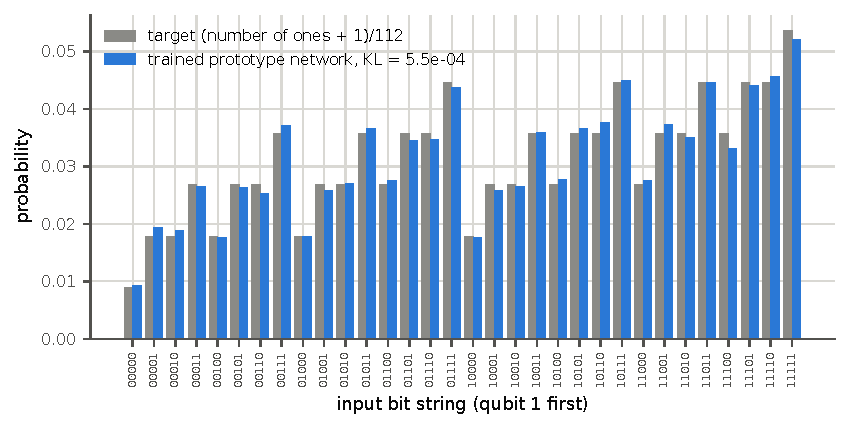
\includegraphics[width=\columnwidth]{fig_bitcount_histograms}
\caption{Target histogram (grey) and the trained prototype network's model distribution
(blue) over the 32 input strings; $\KL=5.5\times10^{-4}$.  Run
\run{bitcount\_noise/20260820T145335Z}, seed 1.}
\label{fig:agentic-histograms}
\end{figure}

\begin{figure}[tb]
\centering
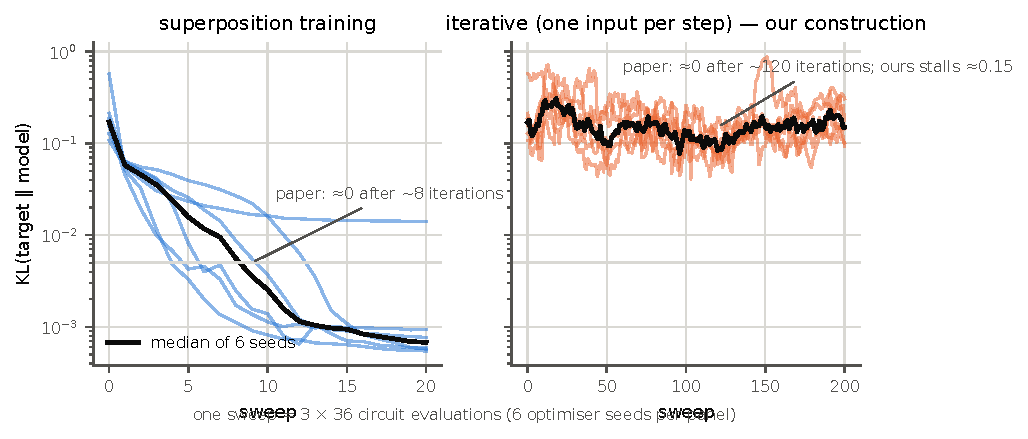
\includegraphics[width=\columnwidth]{fig_bitcount_convergence}
\caption{Left: superposition training, six optimiser seeds and their median.  Right: the
reimplementation's construction of the iterative baseline, which does not reach the
published curve.  Run \run{bitcount/20260820T135930Z}.}
\label{fig:agentic-convergence}
\end{figure}

\subsection{Iris}
\label{app:iris}

How the label enters the amplitude is not stated.  The published bar heights --- $1/86$, $4/86$,
$9/86$ on the training set and $1/154$, $4/154$, $9/154$ on the test set, two independent
integer normalisations --- fix the weight of class $\ell$ as $\propto(\ell+1)^2$: the amplitude
carries $\ell+1$ and the histogram its square, and no other exponent produces both
normalisations.  The split is not stated either; a stratified one-third training split
(50 flowers) is used.  Each feature is quantised into three $k$-means clusters, giving a 12-bit
one-hot code per flower, and the training set is loaded as one superposition over its distinct
codes; the network has 12 inputs, 4 hidden neurons and one output (17 qubits), against a
classic-neuron network of the same size, with labels predicted by rounding each code's read-out
weight.

In \cref{fig:agentic-iris-losses} the classic network drives its training loss to $10^{-5}$
within a few sweeps while its test loss bottoms out early and stays at $0.03$--$0.04$ --- it
memorises --- whereas the prototype network descends more slowly on both and its test loss is
still falling at sweep~40.  Prototype test accuracy is $95\,\%$, $91\,\%$ and $98\,\%$ on the
three splits against the published $\approx98\,\%$; the encoding caps accuracy at $97\,\%$,
$99\,\%$ and $99\,\%$, since two flowers of different species can share a 12-bit code.  The
t-SNE picture of \cref{fig:tsne} does not reproduce: in this embedding both weight sets cluster
away from the data, and what was plotted is not recoverable from the text.

\paragraph{On the split.}
The published histograms show 15 non-empty bars for the training set and 30 for the test set.
The 50-flower training splits used here give 14, 12 and 14 distinct codes, close to 15, but the
100-flower test splits give only 20, 20 and 18, not 30: three clusters per feature do not
spread 100 flowers over 30 codes on any split tried.  The figure supports the \emph{direction}
of the split, not its ratio, which remains an assumption.  An earlier draft claimed the bar
counts justified the ratio; an independent review caught the over-reading and the justification
was withdrawn.

\begin{figure}[tb]
\centering
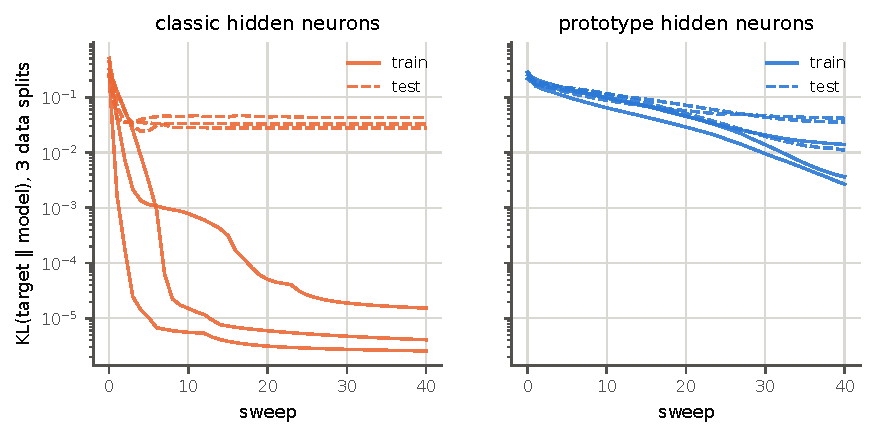
\includegraphics[width=\columnwidth]{fig_iris_losses}
\caption{Training (solid) and test (dashed) loss per sweep on three data splits, classic
against prototype network.  Runs \run{iris/20260820T144849Z}, \run{...T145454Z},
\run{...T145455Z}.}
\label{fig:agentic-iris-losses}
\end{figure}

\subsection{Flappy Bird}
\label{app:flappy}

The submission gives no reward, no training protocol and no game constants, so a
deterministic, window-free clone was built.  Its physics are a choice: the classic constants
(impulse $-9$, gap 100, spacing 144) are provably unplayable by a memoryless two-feature policy
--- one flap overshoots by 40.5\,px against a 38\,px budget --- so impulse $-7$, gap 120,
spacing 180 are used.  Height and the centre of the next gap enter two input qubits by
\cref{eq:agentic-encoding}; four prototype hidden neurons and one classic output flap when
$\Pout>\tfrac12$, 17 angles in all.  Training minimises the negative episode return (0.01 per
frame, 1 per pipe) plus a tracking term $|{\rm height}-{\rm gap}|$ supplying a slope where
every policy dies within 30 frames; 300 random vectors are scored on short episodes and the
best seeds 25 sweeps on five 1500-frame episodes.

The trained network passes 110 pipes in 5\,000 frames --- the cap, a perfect game --- on
all 20 held-out game seeds, for all 8 optimiser seeds tried, in about three minutes of training
(run \run{flappy/20260820T143753Z}); \cref{fig:agentic-flappy-policy} shows the learned
boundary.

\begin{figure}[tb]
\centering
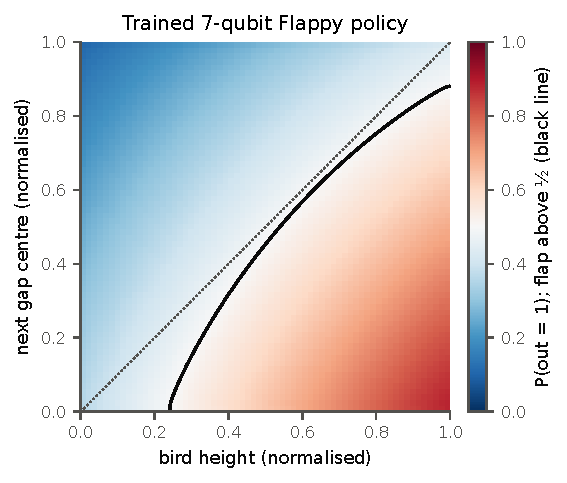
\includegraphics[width=0.85\columnwidth]{fig_flappy_policy}
\caption{The trained controller's activation $\Pout$ over the two observations; the black
line is the decision boundary $\Pout=\tfrac12$ (flap to its right), the dotted diagonal is
``bird at gap height''.  Run \run{flappy/20260820T143753Z}.}
\label{fig:agentic-flappy-policy}
\end{figure}

\subsection{ECG denoising}
\label{app:ecg}

Five consecutive noisy samples enter five input qubits; one to three prototype hidden neurons
and one output predict the clean centre sample as $\Pout$.  The recording is not identified;
the published trace is a smooth two-beat signal of 1\,800 samples in $[0,1]$ with additive
noise of standard deviation $\approx0.03$.  A synthetic ECG of McSharry form was generated to
match it, Gaussian noise of $\sigma=0.02$ added (noisy input $32.0$~dB), the first half used
for training and the second for test, and the experiment repeated on PhysioNet MIT-BIH
record~100~\cite{moody2001mitbih}.

PSNR is $37.4$, $38.0$ and $38.1$~dB for one, two and three prototype neurons against the
published $32.9$, $40.00$ and $40.04$: within about $2$~dB at two and three neurons, and $4$~dB
\emph{above} the published value at one neuron (\cref{fig:agentic-ecg-trace}).  The prototype
network beats the classic one at one and two neurons and on every SSIM; the classic one wins at
three.  The numbers cannot match exactly because the signal is not the authors' own.  The
alternative encoding $\theta=\pi s$ costs $0.6$--$7$~dB here, independent evidence for
\cref{eq:agentic-encoding}.  On MIT-BIH record~100 (run \run{ecg/20260820T165912}) the same
networks reach $36$--$38$~dB.

\begin{figure}[tb]
\centering
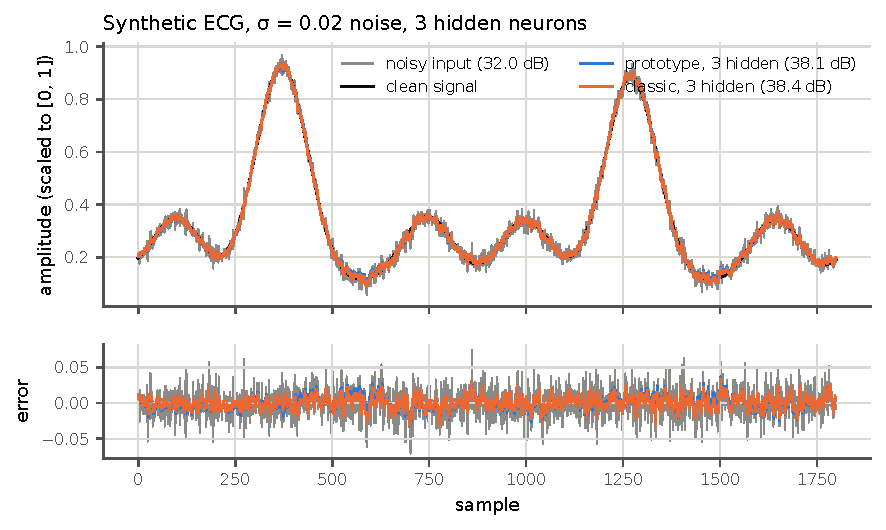
\includegraphics[width=\columnwidth]{fig_ecg_trace}
\caption{Noisy input, clean signal and the two three-neuron networks' outputs (top); their
errors (bottom).  Run \run{ecg/20260820T162014}.}
\label{fig:agentic-ecg-trace}
\end{figure}


\section{The experiments under calibrated noise}
\label{app:noise}

\subsection{Seven machines as noise models}
\label{app:devices}

Each vendor's published gate errors, gate durations, $T_1$, $T_2$, readout error and
connectivity were collected into a device file whose every field carries its source URL,
retrieval date (20 August 2026) and a verbatim quotation (\cref{app:provenance});
\cref{tab:agentic-devices} summarises them.  Three caveats govern everything that follows.
\emph{Quantinuum publishes no gate durations and no $T_1$/$T_2$}: its idle error is charged
from its published memory error per depth-1 circuit time ($2.0\times10^{-4}$ for H2-1,
$2.2\times10^{-4}$ for H1-1), and its simulated noise carries no idle error.  \emph{Rigetti
publishes only a two-qubit error} for Ankaa-3, its $99.5\,\%$ headline being for a different
gate than the universal one needed here, so every Rigetti number is an upper bound.
\emph{IQM's $T_1$/$T_2$ are a third-party snapshot}, and its $T_2$ without echo is $8.5\,\mu$s
against the $21\,\mu$s echo value used.  Where a vendor publishes nothing, the channel is
modelled as error-free and flagged, not invented.

\begin{table*}[t]
\caption{The seven device presets (medians where the vendor publishes per-qubit tables).
Two-qubit error $\varepsilon_2$, one-qubit error $\varepsilon_1$, readout error (mean of
$p_{01}$, $p_{10}$), coherence times, two-qubit gate time.  ``---'' = not published.}
\label{tab:agentic-devices}
\begin{tabular}{@{}l l S[table-format=1.2e-1] S[table-format=1.1e-1] S[table-format=1.1e-1] l l S[table-format=6.0]@{}}
\toprule
Machine & Connectivity & {$\varepsilon_2$} & {$\varepsilon_1$} & {readout} & $T_1$ & $T_2$ & {2q gate (ns)} \\
\midrule
Quantinuum H1-1 & all-to-all & 9.7e-4 & 1.8e-5 & 2.3e-3 & --- & --- & {---} \\
Quantinuum H2-1 & all-to-all & 1.1e-3 & 1.9e-5 & 1.0e-3 & --- & --- & {---} \\
IonQ Forte & all-to-all & 4.0e-3 & 2.0e-4 & 5.0e-3 & 55\,s & 1\,s & 950000 \\
Google Willow & square & 4.1e-3 & 5.3e-4 & 8.0e-3 & $68\,\mu$s & $89\,\mu$s & 42 \\
IBM Fez (Heron r2) & heavy-hex & 3.9e-3 & 2.3e-4 & 7.7e-3 & $145\,\mu$s & $88\,\mu$s & 84 \\
IQM Garnet & square & 4.9e-3 & 8.0e-4 & 3.0e-2 & $27\,\mu$s & $21\,\mu$s & 30 \\
Rigetti Ankaa-3 & square & 1.0e-2 & {---} & {---} & --- & --- & 72 \\
\bottomrule
\end{tabular}
\end{table*}

\subsection{Bit-count}
\label{app:noise-bitcount}

The trained 11-qubit networks were evaluated exactly, as density matrices on the GPU, under
each preset (run \run{bitcount\_noise/20260820T145335Z};
\cref{fig:agentic-noise-devices}).  The model distribution moves by $\TV=0.005$ (Quantinuum
H2-1) to $0.039$ (IQM Garnet), and the KL to the target rises from $5.5\times10^{-4}$ to
$7\times10^{-4}$ on H2-1 and to $6\times10^{-3}$ on Garnet.  The prototype network is better
under every preset, but the displacement \emph{caused} by the noise,
$\KL(\text{clean}\,\|\,\text{noisy})$, is the same for both (median $0.0021$ against $0.0022$):
they have identical two-qubit gate counts, so the prototype's advantage under noise is
inherited from its better noiseless fit, not from robustness of the neuron type.  Scaling IBM
Fez's noise by $s$ gives $\KL\propto s^{1.7}$ and $\TV\propto s^{0.95}$.

Training \emph{under} the noise works, on a 7-qubit version (3 inputs, 3 hidden; the 11-qubit
grid would have cost 13 hours and was not run): it recovers the noisy KL by a median factor of
$158$ (prototype) and $361$ (classic), \cref{fig:agentic-noise-aware}.  But the recovered
parameters are \emph{worse} on a noiseless simulator --- the optimiser folds the channel into
the angles instead of finding noise-robust ones.

\begin{figure}[tb]
\centering
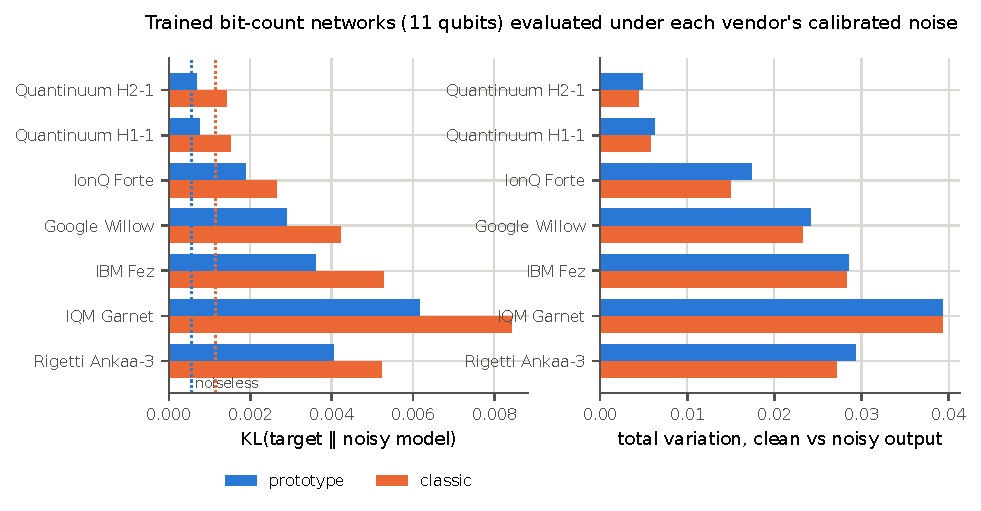
\includegraphics[width=\columnwidth]{fig_bitcount_noise_devices}
\caption{The trained bit-count networks under each machine's noise model.  Left: KL to the
target, noiseless values dotted.  Right: how far the output distribution moved.  Rigetti's
row models only its two-qubit error.  Run \run{bitcount\_noise/20260820T145335Z}.}
\label{fig:agentic-noise-devices}
\end{figure}

\begin{figure}[tb]
\centering
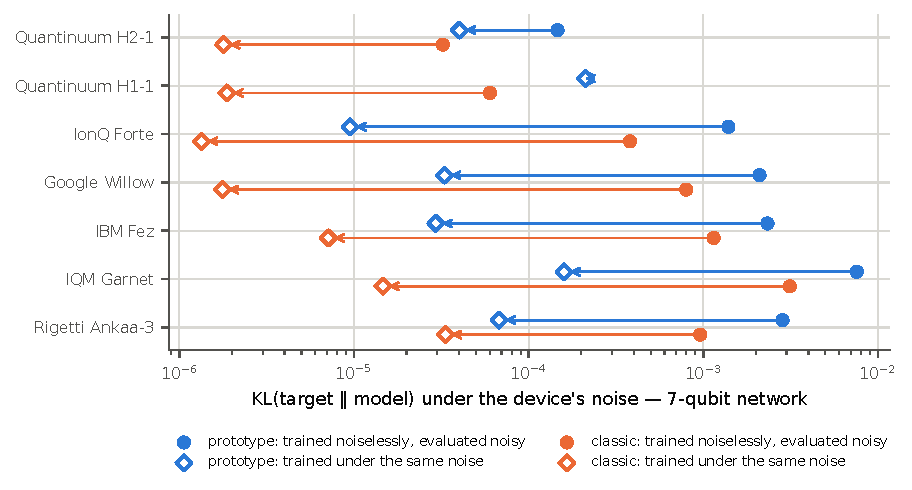
\includegraphics[width=\columnwidth]{fig_bitcount_noise_aware}
\caption{Noise-aware training of the 7-qubit bit-count network: KL under each machine's noise
for parameters trained noiselessly (filled) and with the same noise model in the loop (open),
median of three seeds.  Same run.}
\label{fig:agentic-noise-aware}
\end{figure}

\subsection{Flappy Bird}
\label{app:noise-flappy}

For a thresholded activation what matters is not how far $\Pout$ moves but whether it crosses
$\tfrac12$.  Evaluated exactly under every preset on its $65\times65$ decision grid and played
for 20 held-out games (run \run{flappy\_noise/20260820T154249Z};
\cref{fig:agentic-flappy-noise}), the controller \emph{still plays perfectly on all seven
machines}: only $1.5$--$4\,\%$ of visited frames are decided differently, because the noise
contracts every activation toward $\tfrac12$ by about the same amount (mean
$|\Delta P|=0.002$--$0.018$) and so rarely changes the ordering.  There is a factor of two of
headroom: Fez's noise scaled by $2$ leaves $60\,\%$ of games perfect, by $4$ none.

Shot noise is a different matter (\cref{fig:agentic-flappy-shot-noise}).  Re-deciding every
frame from $N$ measurements, the controller wins no game at $N=1\,000$, $90\,\%$ at $4\,000$
and all at $10\,000$ noiselessly; on Fez's model only $55\,\%$ at $4\,000$.  The cause is the
margin distribution over played frames: median $\delta=0.019$, tenth percentile $0.004$, first
percentile $0.0002$; the measured flip rate agrees with the average of $\Phi(-2\delta\sqrt N)$
over it to $3\,\%$.  A deterministic shift of the boundary is tolerated far past a stochastic
one --- Fez at scale $2$ decides $20\,\%$ of frames differently and still wins $60\,\%$ of
games, while $1\,000$ shots decide only $8.5\,\%$ differently and win none ---.  Fine-tuning under Fez's noise for five sweeps changes nothing: the training
episodes all survive already, so the objective has no slope.

\begin{figure}[tb]
\centering
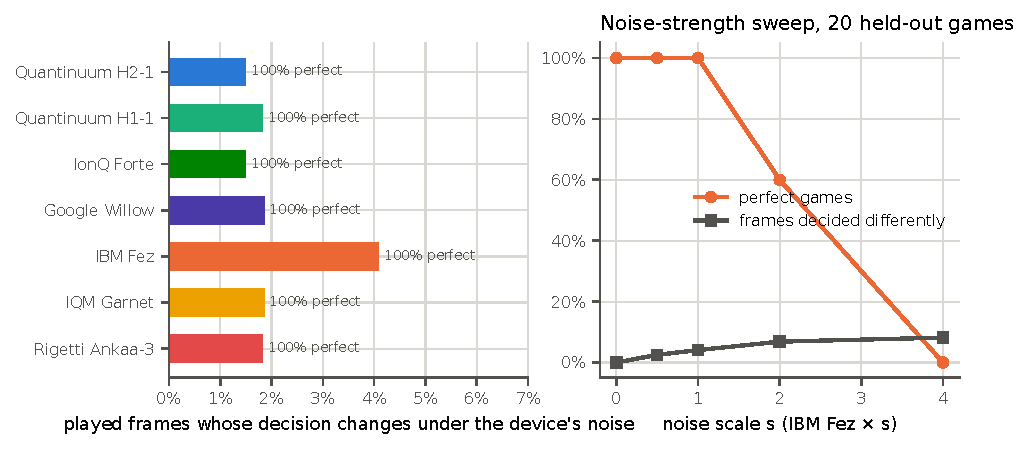
\includegraphics[width=\columnwidth]{fig_flappy_noise}
\caption{Flappy under gate noise.  Left: fraction of played frames whose decision changes
under each machine's model; every machine still yields $100\,\%$ perfect games.  Right: IBM
Fez's noise scaled by $s$.  Run \run{flappy\_noise/20260820T154249Z}.}
\label{fig:agentic-flappy-noise}
\end{figure}

\begin{figure}[tb]
\centering
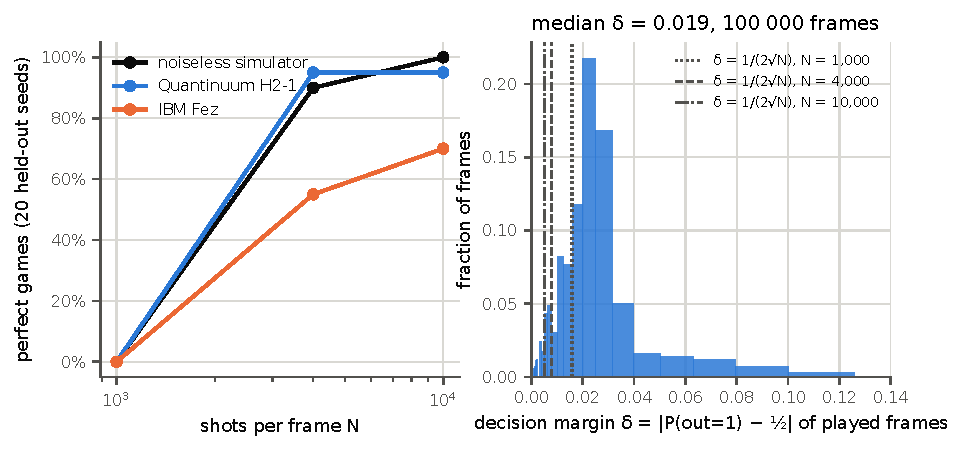
\includegraphics[width=\columnwidth]{fig_flappy_shot_noise}
\caption{Flappy under shot noise.  Left: perfect games when every frame is decided from $N$
shots.  Right: distribution of the decision margin $\delta$ over the $100\,000$ frames the
noiseless controller plays; vertical lines mark the margin that $N$ shots can just resolve.
Same run.}
\label{fig:agentic-flappy-shot-noise}
\end{figure}

\subsection{ECG and Iris, reduced run}
\label{app:noise-ecg-iris}

These two grids were run in a \emph{reduced} configuration only (run
\run{ecg\_iris\_noise/20260820T155618Z}): ECG on 8 test windows instead of 898 and two presets
instead of seven; Iris with 16 Monte-Carlo trajectories per evaluation instead of 2\,000
(per-outcome standard error $\approx12\,\%$), two presets, and perfect preparation of the
dataset state assumed.  The full grids cost 4--6 CPU-hours (ECG) and 8 hours (Iris), outside
the budget.  The results (\cref{fig:agentic-ecg-iris-noise}) are indicative only: ECG loses
$-0.1$ to $+0.4$~dB under Quantinuum H2-1 and $1.6$--$2.7$~dB (classic) under IBM Fez, while
the prototype cells \emph{gain} up to $3.8$~dB under Fez on eight windows --- a small-sample
artefact, not a finding.  Iris keeps its $95\,\%$ accuracy under H2-1 and loses it under Fez
($64\pm44\,\%$ over two trajectory seeds) for the prototype network, whose read-out is a
conditional distribution over 4\,096 input strings and is therefore directly exposed to
probability leaking out of the 20-code support.  One noisy sweep of ECG fine-tuning gains
$2.7$~dB under Fez and $3.7$~dB noiselessly: it finishes the clean optimisation, it does not
fold the channel in.

\begin{figure}[tb]
\centering
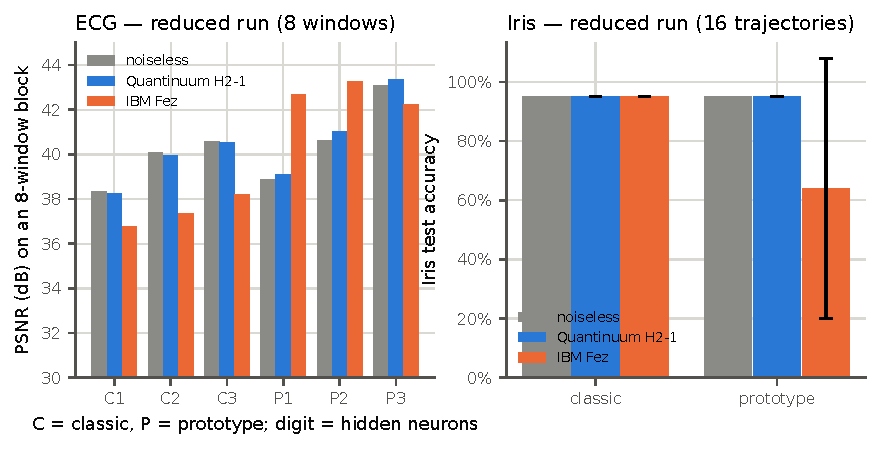
\includegraphics[width=\columnwidth]{fig_ecg_iris_noise}
\caption{Reduced-configuration noise runs, quoted for the record.  Left: ECG PSNR on an
8-window block.  Right: Iris test accuracy from 16 trajectories, error bars over two
trajectory seeds.  Run \run{ecg\_iris\_noise/20260820T155618Z}.}
\label{fig:agentic-ecg-iris-noise}
\end{figure}


\section{What it takes to run this on a real machine}
\label{app:hardware}

All numbers here are printed by one script into \run{hardware-plan/20260821T084554Z} (file
\code{numbers.md}); it joins every calibration number to its provenance entry and refuses to
run if one is missing.

\subsection{Compilation}
\label{app:compile}

Every prototype neuron touches every input, so the two-qubit gates form a complete bipartite
graph between inputs and hidden qubits --- the worst case for a lattice.  On an all-to-all
machine each controlled rotation costs exactly two native two-qubit gates: 24 for Flappy, 60
for bit-count.  On a lattice the compiler must insert SWAPs at three native gates each; with a
greedy router the bit-count circuit needs 327 native two-qubit gates on IBM's heavy-hex lattice
and 207 on a square lattice, $82\,\%$ and $71\,\%$ of them SWAP-borne
(\cref{fig:agentic-entanglers}).  IBM's own compiler needs 97 at optimisation level~2,
$3.4\times$ fewer, so this router is a device-independent comparison instrument and not what
one would submit.  The Flappy circuit is $12.9\,\mu$s long on Fez ($1.56\,\mu$s of it readout)
and 17.9\,ms on IonQ Forte, whose gates take a millisecond.

\begin{figure}[tb]
\centering
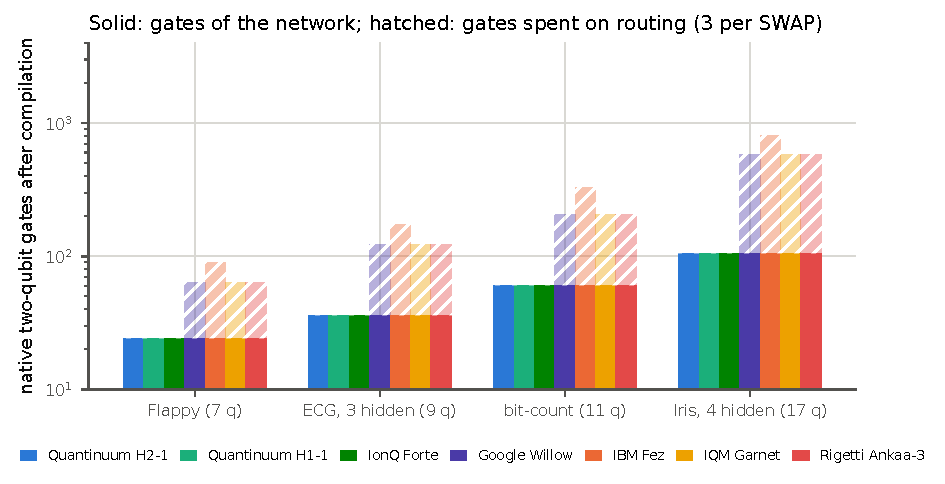
\includegraphics[width=\columnwidth]{fig_hardware_entanglers}
\caption{Native two-qubit gates after compiling each network for each machine (greedy router,
log scale).  All-to-all machines need only the network's own gates; the lattices spend most of
their budget on routing.  Run \run{hardware-plan/20260821T084554Z}.}
\label{fig:agentic-entanglers}
\end{figure}

\subsection{Expected fidelity}
\label{app:fidelity}

\Cref{fig:agentic-fidelity} stacks the four factors of \cref{eq:agentic-fidelity} for the two
smallest circuits, with the exactly simulated total-variation distance between the compiled
circuit run clean and run under noise beside each bar.  Flappy at 7 qubits is a high-fidelity
circuit on trapped ions ($F\approx0.92$ on H2-1, $0.83$ on Forte), marginal on Willow and Fez
($0.63$; $0.46$ with the greedy router, $0.75$ with IBM's compiler) and poor on Garnet
($0.24$).  Bit-count at 11 qubits is feasible on the H-series ($0.81$) and Forte ($0.64$),
usable with IBM's compiler on Fez ($0.48$) and dead on Garnet ($0.008$), whose routed circuit
lasts $86\,\%$ of its $T_2$.  Idling is charged only over each qubit's schedule gaps, since
relaxation during a gate is already inside the vendor's gate error; charging the whole circuit
duration on every qubit is $10$--$15$ points more pessimistic on the superconducting machines
and is printed beside it in the run directory.

Two cautions.  The simulated distances of the \emph{compiled} circuits ($0.03$ on the H-series,
$0.16$ on Forte, $0.43$ on Fez) are $5$--$15\times$ larger than for the uncompiled circuits of
\cref{app:noise-bitcount}.  And vendors' two-qubit errors are measured in isolation --- IBM's
own layered benchmark for Fez is $1.7\times$ worse than its isolated gate error --- so the
lattice numbers are optimistic.

\begin{figure*}[t]
\centering
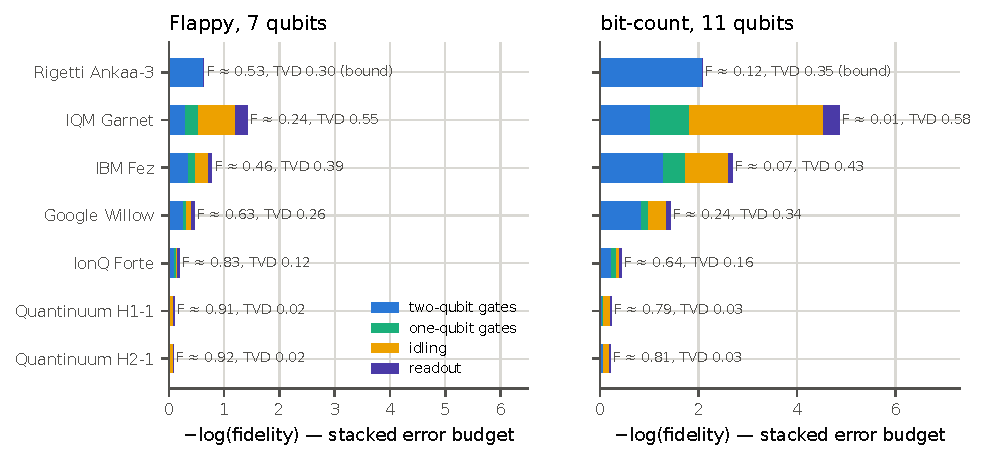
\includegraphics[width=0.92\textwidth]{fig_hardware_fidelity}
\caption{Error budget per machine for the Flappy (left) and bit-count (right) circuits: the
stacked bars are $-\log$ of each factor of \cref{eq:agentic-fidelity}, so their total is
$-\log F$; labels give $F$ and the simulated total-variation distance of the compiled circuit.
Quantinuum's idle term comes from its published memory error; Rigetti's is a bound from its
two-qubit error only.}
\label{fig:agentic-fidelity}
\end{figure*}

\subsection{Shots, time and money}
\label{app:cost}

An activation to $\pm0.005$ needs $10\,000$ shots.  The 32-bin bit-count histogram is estimated
from the shots in which the output fired ($\Pout=0.487$ of them), so the plug-in KL is biased
upward by $(K-1)/(2\cdot0.487\cdot N)=31.8/N$ with $K=32$; reaching the trained model's
$5.5\times10^{-4}$ needs $58\,000$ shots, rounded to a $64\,000$-shot job.  The ECG PSNR is
capped by shot noise at $10\log_{10}(4N)$, so $2\,500$ shots per sample cap it at exactly
$40$~dB --- the published Table~I value --- and a $1\,800$-sample trace at $25\,000$ shots is
$4.5\times10^7$ shots: ECG is a simulator experiment.  Machine time per job is milliseconds to
two seconds on the superconducting machines, where the per-job overhead dominates, but $72$\,s
(Flappy) and 32 minutes (bit-count) on IonQ Forte, where circuit time does.

Prices retrieved 20 August 2026 are in \cref{tab:agentic-cost}.  Training on hardware is out of
the question: $2\,160$ evaluations at $64\,000$ shots are $1.4\times10^8$ shots, 48 days of
Forte time or \$11\,M.  Fine-tuning the six output angles (90 evaluations at $4\,000$ shots) is
$1.8$ hours on Forte, about 45 minutes on Fez.  Live play is equally out: $1\,500$ frames
$\times$ $4\,000$ shots $\times$ $17.9$\,ms is 30 hours per episode on Forte.  The falsifiable
hardware observable is instead the activation map of \cref{fig:agentic-flappy-policy} on a grid
of observations, 16 jobs.

\begin{table*}[t]
\caption{Cost per job (file \code{numbers.md}, section ``cost'').  IBM: \$1.60 per QPU second
plus a 30\,s per-job overhead, both assumptions (\cref{app:assumptions}); Quantinuum: the
vendor's credit formula converted at the Azure plan rate; Braket: published per-shot prices.}
\label{tab:agentic-cost}
\begin{tabularx}{\textwidth}{@{}l X l l@{}}
\toprule
Machine & Price model & Flappy, 4\,000 shots & bit-count, 64\,000 shots \\
\midrule
IBM Fez & \$1.60/s; 52\,ms resp.\ 1.8\,s of QPU & \$0.08 (\$48 with overhead) & \$2.85 (\$51) \\
IBM Open plan & 10 min per 28 days, free & \$0 & \$0 \\
Quantinuum H1/H2 & credits $=5+(N_1+10N_2+5N_m)C/5000$ & 323 credits $\approx$ \$4\,030 & 11\,920 credits $\approx$ \$149\,000 \\
IonQ Forte (Braket) & \$0.30 + \$0.08/shot & \$320 & \$5\,120 \\
IQM Garnet (Braket) & \$0.30 + \$0.00145/shot & \$6.10 & \$93 \\
\bottomrule
\end{tabularx}
\end{table*}

\subsection{Recommendation}
\label{app:recommendation}

Run the 7-qubit Flappy activation map first: on IBM's free plan to debug the pipeline (readout
calibration, then zero-noise extrapolation by gate folding, both validated offline against the
noise model), then on IonQ Forte for the confirmation (\$1\,300 for a $4\times4$ grid at
$1\,000$ shots), and on Quantinuum H2-1 for the headline number if an allocation exists.  The
bit-count histogram is feasible on the H-series and Forte as a \emph{shape} demonstration but
not as a KL comparison: device error puts the KL floor at $10^{-2}$--$10^{-1}$, two orders
above the simulated $5.5\times10^{-4}$.  Iris cannot be settled yet.  What these runs prepare
is a uniform superposition over the $12$--$14$ \emph{distinct} training codes, not over the 120
samples an earlier draft assumed; the sparse state-preparation construction of Gleinig and
Hoefler~\cite{gleinig2021sparse} has leading term $k\cdot n=144$--$168$ two-qubit gates, giving
$F\approx0.83$ on H2-1 and $\approx0.75$ with the network --- but its constant is unknown, and
the dense alternatives ($8\,168$ gates by Shende--Bullock--Markov synthesis, $\approx3\,925$ by
Plesch--Brukner) are hopeless.  An exact answer needs an actual sparse state-preparation
circuit, which the repository does not build.  For a live submission the code still lacks
credentials, the vendors' own routing, asynchronous job handles, and readout-unfolding and
gate-folding utilities.


\section{The shot-noise programme}
\label{app:shots}

What limits a hardware demonstration is the number of measurements, through two mechanisms: a
thresholded controller flips at a rate $\Phi(-2\delta\sqrt N)$, and a histogram loss estimated
from $N$ shots is biased upward by $(K-1)/(2\,\Pout\,N)$ while discarding the half of the shots
in which the output did not fire.  Six remedies were proposed and three implemented.  The
others --- a joint-distribution loss or amplitude amplification so that all shots are used,
bias-corrected KL estimators, and amplitude estimation --- are designed but not implemented;
the first is the natural next step, since the estimator bias is what now limits sampled
training.  All runs here are noiseless state-vector simulations plus sampling.

\subsection{Margin-aware training: negative}
\label{app:margin}

If every frame had $\delta\ge0.1$ instead of the median $0.019$, the shots per frame would fall
by $(0.1/0.019)^2\approx25\times$ at no noiseless cost.  A penalty
$w\times0.01\times\max(0,1-\delta/m)$ per played frame was added --- a fraction $w<1$ of the
$0.01$ reward for surviving that frame, so surviving always beats dying confidently --- and the
controller fine-tuned for 25 sweeps with $m=0.1$, $w\in\{0.25,0.5,1\}$ (run
\run{flappy\_shots/20260821T084601Z}).  An earlier attempt with a \emph{mean} hinge of weight
20, trained from scratch, collapsed to a policy that died in 30 frames with perfectly confident
decisions (run \run{flappy\_shots/20260821T075048Z}): any penalty that can outweigh the
per-frame reward selects for dying early.

The margin quantiles hardly move (\cref{fig:agentic-flappy-shots}, left; median
$0.019\to0.021$--$0.024$, tenth percentile $0.004\to0.006$).  All three fine-tuned controllers
still play perfectly on exact probabilities, but under shot noise they play \emph{worse} than
the original at $w\ge0.5$ ($50\,\%$ and $80\,\%$ perfect games at $10\,000$ shots against
$100\,\%$).  The near-boundary frames are those in which the bird hovers at the boundary, a
property of the game's dynamics and not of the surface's steepness, so penalising them moves
the boundary rather than steepening it --- and a 17-parameter network has no spare capacity to
steepen its surface anyway.

\subsection{Common random numbers}
\label{app:crn}

A slope from $N$ independent shots per probe with variance $\sigma^2$ has variance
$\sigma^2/2c^2$, at $c=0.2$ some $12.5\sigma^2$, which is why finite differences on a sampling
backend stall.  Feeding the same uniform random numbers to both probes gives only a
$1.3\times$ reduction, because a parameter change moves probability between distant bit strings
and shifts every later bin boundary.  What works is the \emph{maximal coupling}: sample the
first probe, then for the second keep each outcome $i$ with probability
$\min(1,p_{\mathrm{new}}(i)/p_{\mathrm{ref}}(i))$ and redraw otherwise from
$(p_{\mathrm{new}}-p_{\mathrm{ref}})_+$.  The second sample has exactly the right distribution
and only $N\cdot\TV(p_{\mathrm{new}},p_{\mathrm{ref}})$ shots change; since $\TV\propto c$, the
slope's variance is $O(1/(cN))$ rather than $O(1/(c^2N))$, a gain of order $1/c$.  Coupling
reduces the variance of the slope, not the bias of a non-linear loss.  On hardware the analogue
is to interleave the $\pm c$ circuits in one job so they share the same drift.

Measured on one slope of the bit-count loss at 400 shots per probe, the reduction is
$\times2$--$3$ at $c=0.2$--$0.4$ and $\times22$--$29$ at $c=0.025$--$0.05$, both estimates
unbiased for the exact slope.  Training the 11-qubit network on a sampling backend (run
\run{bitcount\_shots/20260821T084558Z}) gives, after 20 sweeps, an exact KL improving from
$0.080$ to $0.059$ at $N=1\,000$ shots per evaluation, from $0.050$ to $0.014$ at $4\,000$, and
at $16\,000$ the two are within the seed-to-seed spread ($0.029$ against $0.033$) --- all an
order of magnitude above the exact-probability result ($0.0009$).  The likely reason is the
loss itself: a plug-in KL of a 32-bin histogram from about $N/2$ usable shots, biased by
$31.8/N$, with the reached KL tracking one to three times that bias.  Three seeds, one of which
stalls at $0.014$ even on exact probabilities, cannot separate estimator from optimiser; a
bias-corrected or joint loss under paired initialisations is the test, and it has not been run.
The schedule used ($c_0=0.2$ decaying only to $0.15$ over 20 sweeps) also keeps the optimiser
where the reduction is smallest.

\subsection{Sequential decisions: positive}
\label{app:sprt}

A fixed budget wastes most of its shots: a frame with $\delta=0.3$ is decided correctly after a
dozen.  Wald's sequential probability ratio test~\cite{wald1945} between
$\Pout=\tfrac12\pm\delta_0$ draws shots in blocks, computes after $n$ shots with $k$ ones the
log-likelihood ratio $\Lambda=(2k-n)\log\frac{1+2\delta_0}{1-2\delta_0}$, and stops when
$\Lambda\ge\log\frac{1-\beta}{\alpha}$ (flap) or $\Lambda\le\log\frac{\beta}{1-\alpha}$ (do
not), up to a cap after which the majority decides.  Beyond $\delta_0$ its error probability is
at most about $\alpha$ ($=\beta=5\,\%$ here); nearer the boundary it is slow and unbounded.

On the same 20 held-out games (\cref{fig:agentic-flappy-shots}; \cref{tab:agentic-sprt}) the
rule with $\delta_0=0.01$ and cap $10\,000$ wins \emph{every} game at a mean of $2\,191$ shots
per frame, against the $10\,000$ a fixed budget needs for the same result --- $4.6\times$ fewer
--- and with $\delta_0=0.005$, cap $4\,000$ it matches the fixed $4\,000$-shot result
($85\,\%$) at $2\,916$.  Setting $\delta_0$ at the median margin ($0.02$) fails ($30\,\%$
perfect at $822$ shots): the frames that decide a game are the near-boundary ones, so the
indifference margin must sit below \emph{their} margins, the tenth percentile of
$0.004$--$0.006$.  The rule needs no change to the network and no retraining.

\begin{figure*}[t]
\centering
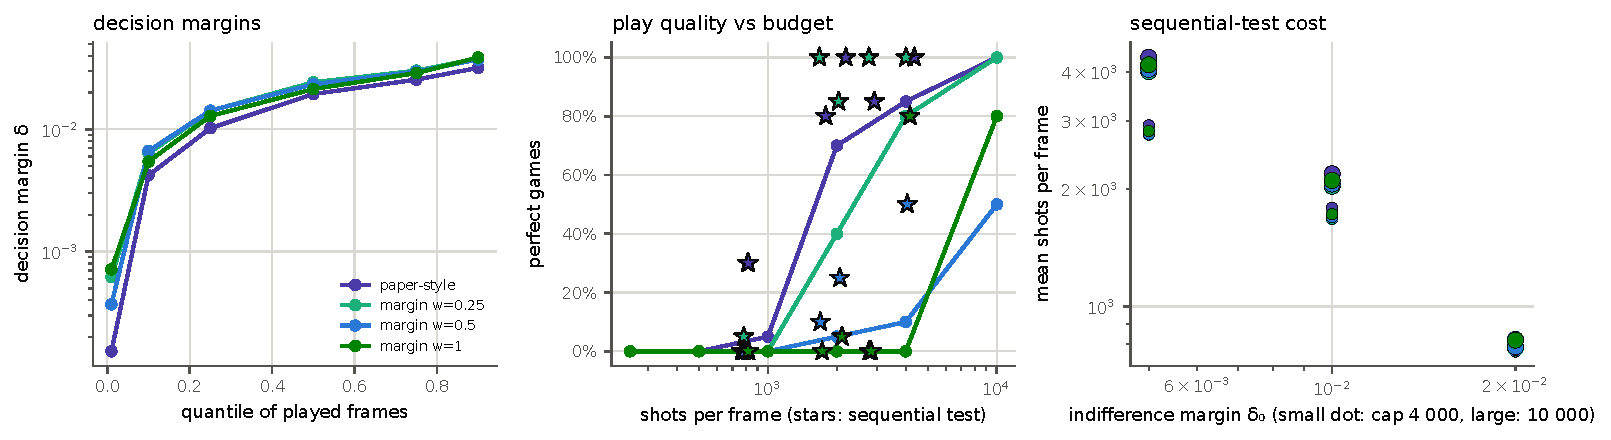
\includegraphics[width=\textwidth]{fig_flappy_shots_programme}
\caption{Flappy under shot noise, remedies 1 and 3.  Left: decision-margin quantiles of the
frames played by the original and the three margin-aware controllers.  Middle: perfect games
against shots per frame for a fixed budget (lines) and for the sequential test (stars, plotted
at the mean number of shots it actually spent).  Right: mean shots per frame of the sequential
test against its indifference margin $\delta_0$.  Run
\run{flappy\_shots/20260821T084601Z}.}
\label{fig:agentic-flappy-shots}
\end{figure*}

\begin{table*}[t]
\caption{Flappy, original controller, 20 held-out games: fixed shot budgets against the
sequential test ($\alpha=\beta=0.05$, blocks of 20 shots).  ``Flips'' are frames decided
differently from the exact rule.  Run \run{flappy\_shots/20260821T084601Z}.}
\label{tab:agentic-sprt}
\begin{tabular}{@{}l S[table-format=3.0] S[table-format=3.0] S[table-format=2.2] S[table-format=5.0]@{}}
\toprule
Decision rule & {perfect games (\%)} & {median pipes} & {flips (\%)} & {mean shots/frame} \\
\midrule
fixed $N = 1\,000$ & 5 & 23 & 8.36 & 1000 \\
fixed $N = 2\,000$ & 70 & 110 & 7.40 & 2000 \\
fixed $N = 4\,000$ & 85 & 110 & 6.09 & 4000 \\
fixed $N = 10\,000$ & 100 & 110 & 4.47 & 10000 \\
sequential, $\delta_0 = 0.02$, cap $10\,000$ & 30 & 88 & 7.19 & 822 \\
sequential, $\delta_0 = 0.01$, cap $4\,000$ & 80 & 110 & 6.12 & 1790 \\
sequential, $\delta_0 = 0.005$, cap $4\,000$ & 85 & 110 & 5.98 & 2916 \\
sequential, $\delta_0 = 0.01$, cap $10\,000$ & 100 & 110 & 5.06 & 2191 \\
sequential, $\delta_0 = 0.005$, cap $10\,000$ & 100 & 110 & 4.50 & 4358 \\
\bottomrule
\end{tabular}
\end{table*}


\section{What the reproduction learned}
\label{app:learnings}

\begin{enumerate}
\item \textbf{The central claims reproduce.}  Activation surface, bit-count histogram and
convergence, Iris overfitting contrast, perfect Flappy play on a clone, ECG denoising within
2~dB on a different signal.  What does not: the iterative baseline of \cref{fig:OptConv} (this
construction stalls at $\KL\approx0.15$) and the weight picture of \cref{fig:tsne}; both are
under-specified in the text.

\item \textbf{Reading figures is part of reproduction.}  The bit-count target
$(\text{ones}+1)/112$, the Iris label weighting $(\ell+1)^2$ and the angle encoding
$\theta=2\arcsin\sqrt s$ were all read off figures and then confirmed to the figure's
precision.  Where a figure was over-read --- the Iris split ratio --- an independent review
caught it and the justification was withdrawn (\cref{app:iris}).

\item \textbf{The prototype network's advantage under noise is inherited, not intrinsic.}  Both
networks have the same two-qubit gate count and the noise displaces both equally; the prototype
wins under noise because it fits better without it.

\item \textbf{Gate noise at published levels is not the obstacle; shots are.}  Every
7--11-qubit network survives every vendor's calibrated model with a qualitatively intact
result, while the Flappy controller needs $10^4$ shots per frame at a fixed budget and the
bit-count loss is biased by $31.8/N$.  The one remedy that pays now is the sequential rule
($4.6\times$ fewer shots, no retraining); margin-aware training does not work for a
17-parameter network; common random numbers reduce the optimiser's noise by $1/c$ but leave the
estimator's bias, the likely and as yet untested limit of sampled training.

\item \textbf{Compiled circuits are $5$--$15\times$ more noise-sensitive than logical ones.}
Two native gates per controlled rotation, resynthesised single-qubit gates and lattice routing
all cost; a complete-bipartite network is the worst case for a lattice, so the vendor's own
compiler must be used for any superconducting submission.  Trapped ions are the natural home of
this architecture, at the price of circuit time.

\item \textbf{An optimiser that keeps a stale incumbent turns a harmless change into a negative
result.}  The ``rotating episodes break training'' finding was an artefact of comparing losses
measured on different episode batches, because the optimiser kept its incumbent's loss from the
previous batch; re-scoring the incumbent on each batch restores $25/25$ perfect games (runs
\run{flappy/batch0}, \run{flappy/batch5}).  Any non-stationary objective needs this.

\item \textbf{Penalties must be priced in the currency of the reward.}  A margin hinge able to
outweigh the per-frame survival reward produced a confidently dead controller; the per-frame
form, kept below that reward, does not.

\item \textbf{Provenance has to be mechanical.}  The first hardware plan contained a dozen wrong
numbers: a state-preparation gate count off by a factor of two, a reversed inequality, costs
computed by hand.  The fix was a script that emits every number and refuses to run if any
calibration input lacks a source; this appendix quotes only that script.
\end{enumerate}


\section{Choices the submission leaves open}
\label{app:assumptions}

Each entry is marked \code{[ASSUMPTION]} where it enters the code.

\begin{description}
\item[Optimiser schedule.]  $a_n=a_0/(n+1)^{0.602}$, $c_n=c_0/(n+1)^{0.101}$, geometric
cooling; one iteration is a coordinate sweep.  Bit-count: $a_0=20$, $c_0=0.2$, $T_0=0.02$,
cooling $0.7$, 20 sweeps.  Flappy: $a_0=0.4$, $c_0=0.25$, $T_0=0.05$, cooling $0.9$, 25 sweeps
after 300 random restarts.  Iris: $a_0=2$, decay exponent $0.3$, $c_0=0.1$, 40 sweeps.  ECG:
100 sweeps with restarts.
\item[Iterative baseline.]  One optimiser sweep on the squared error of one random input per
iteration.
\item[Angle encoding.]  $\theta=2\arcsin\sqrt s$, pinned by a printed angle in the companion
paper; $\theta=\pi s$ tested as an ablation.
\item[KL regularisation.]  Model probability floored at $10^{-12}$ inside the logarithm.
\item[Iris.]  Stratified one-third training split; flowers sharing a code are merged and their
labels averaged; the KL is normalised over all 4\,096 input strings, since restricting it to
the dataset's codes lets the network exploit interference between examples and reach a training
loss of $10^{-5}$ while reading out at chance; label weight $\propto(\ell+1)^2$; labels
predicted by nearest rounding of the read-out weight.
\item[Flappy.]  Clean-room clone: $288\times512$ screen, flap impulse $-7$, gap 120, pipe
spacing 180, gravity 1; reward 0.01 per frame plus 1 per pipe; tracking term
$|{\rm height}-{\rm gap}|$ with weight 1; 5 training episodes of 1\,500 frames, 20 held-out
seeds 5--24, 5\,000-frame cap (110 pipes); decisions cached on a $65\times65$ grid.
\item[ECG.]  Synthetic McSharry-form signal tuned to the published trace, and MIT-BIH
record 100; Gaussian noise $\sigma=0.02$; mirror-padded edges; first half train, second half
test; PSNR with $R$ the range of the clean signal; SSIM in a 7-sample sliding window.
\item[Noise model.]  Depolarising at the vendor's average gate error, relaxation during gates
and as-soon-as-possible idling, readout confusion; medians where vendors publish per-qubit
tables; no crosstalk, since no vendor publishes a usable number.  Quantinuum's idle error is
charged as $(1-m)^{n_{\rm qubits}\cdot{\rm depth}}$ from its memory error per depth-1 time;
IQM's and Rigetti's unpublished one-qubit gate durations are set to 40\,ns.
\item[Fidelity estimate.]  First-order product of per-gate survival probabilities; readout
factor $(1-(p_{01}+p_{10})/2)^n$.
\item[Costs.]  IBM \$1.60 per QPU second (2022 launch figure, corroborated by a secondary
\$96/min report) plus 30\,s per-job overhead; Quantinuum \$12.5 per credit (Azure Standard plan
divided by its allotment); Braket and Azure per-shot prices as retrieved on 20 August 2026;
Quantinuum's credit formula with $N_m=2\times$ qubits.
\item[State preparation.]  Dense counts $2^{n+1}-2n$ (Shende--Bullock--Markov) and
$\approx\tfrac{23}{24}2^n$ (Plesch--Brukner); sparse \emph{leading term} $k\cdot n$ of an
$O(kn)$ construction~\cite{gleinig2021sparse} with $k$ the $12$--$14$ distinct training codes
actually prepared, its constant unknown.
\item[Compilation.]  Lattice machines are compiled onto a synthetic heavy-hex or square patch
of the circuit's size with a greedy router; Google's and Rigetti's gate sets are rebased
through a generic fallback.  Idle relaxation is charged over each qubit's schedule gaps only.
\item[Shot-noise programme.]  Margin penalty $w\cdot0.01\cdot\max(0,1-\delta/m)$ per frame with
$m=0.1$; sequential test with $\alpha=\beta=0.05$ and blocks of 20 shots; common random numbers
by maximal coupling to the first probe of each coordinate.
\end{description}


\section{Provenance of the calibration data}
\label{app:provenance}

Every calibration number used in \cref{app:noise,app:hardware} is stored in a device file with
a provenance block per field: source URL, kind of source (vendor calibration page, vendor
paper, third-party snapshot), retrieval date and a verbatim quotation of the sentence or table
row the number was read from.  The hardware-plan script joins these blocks to every field it
reads and fails if any is missing; the full join, one row per device and field with quotations,
is the file \code{numbers.md} of run \run{hardware-plan/20260821T084554Z}.  In brief:

\begin{description}
\item[IBM Fez (Heron r2).]  One coherent calibration snapshot, backend version 1.2.8 of
2025-02-26, shipped as \code{props\_fez.json} in \code{qiskit-ibm-runtime}'s fake provider;
medians over 156 qubits and 352 directed CZ edges computed from that table.  The file records
the same chip drifting between CZ error $2.85\times10^{-3}$ (2024-07) and $3.90\times10^{-3}$
(2025-02).
\item[Quantinuum H1-1, H2-1.]  The vendor's performance-validation page: mean two-qubit and
one-qubit infidelities, SPAM error, ``Memory Error per Depth-1 Circuit Time''.  No gate
durations, no $T_1$/$T_2$.
\item[IonQ Forte.]  The vendor's published specification: average gate fidelities, gate
durations, $T_1=55$\,s, $T_2=1$\,s.
\item[Google Willow.]  Supplementary information of the Willow paper (\emph{Nature}, 2024):
gate errors, coherence times, cycle time.  Not publicly accessible; the preset exists for
simulation only.
\item[IQM Garnet.]  Vendor data for gate errors and readout; $T_1$ and $T_2$ (echo) from a
third-party calibration snapshot, two epochs recorded (December 2025, March 2026), with the
caveat that $T_2$ without echo is $\approx8.5\,\mu$s.
\item[Rigetti Ankaa-3.]  Only the two-qubit (iSWAP) error $10^{-2}$ is published for the
universal gate; the $99.5\,\%$ headline refers to the fSim gate.  No one-qubit error, no
readout error, no $T_1$ or $T_2$.
\end{description}

The per-field table is not reproduced here --- some sixty rows with quotations --- but it is
the ground truth every number in this appendix rests on, and it is one command away in the
repository at \repourl.
.
%  Requires % ===========================================================================
%  Preamble additions required by  sec-reproducibility.tex  and  app-agentic.tex
%  ---------------------------------------------------------------------------
%  Paste   % ===========================================================================
%  Preamble additions required by  sec-reproducibility.tex  and  app-agentic.tex
%  ---------------------------------------------------------------------------
%  Paste   \input{ptqnn-agentic-preamble}
%  into main.tex directly AFTER  \usepackage{adjustbox}.
%  That position matters: cleveref must be loaded after hyperref (your line 3)
%  and after amsmath, otherwise it patches the wrong \label.
%  Everything here is guarded with \providecommand: if you already define one
%  of these macros, your definition wins and nothing clashes.
% ===========================================================================

\usepackage{booktabs}   % \toprule \midrule \bottomrule in the appendix tables
\usepackage{tabularx}   % X columns (tab:agentic-scoreboard, -cost)
% siunitx and the ascii package both define \SI, and ascii is loaded first, so
% siunitx would abort with "Command '\SI' already defined".  Hide \SI while
% siunitx loads and hand it straight back to ascii afterwards; nothing here
% uses \SI, only the S table column.
\makeatletter
\ifx\SI\@undefined\else\let\asciiSI\SI \let\SI\@undefined\fi
\makeatother
\usepackage{siunitx}    % S columns (tab:agentic-devices, tab:agentic-sprt)
\makeatletter
\ifx\asciiSI\@undefined\else\let\SI\asciiSI\fi
\makeatother
\usepackage[capitalise,nameinlink]{cleveref}   % <-- must come after hyperref

\sisetup{detect-all}

% --- notation --------------------------------------------------------------
\providecommand{\KL}{D_{\mathrm{KL}}}                 % math mode
\providecommand{\Pout}{P(\mathrm{out}=1)}             % math mode
\providecommand{\TV}{\mathrm{TV}}                     % math mode
\providecommand{\RX}{R_X}                             % math mode
\providecommand{\CRX}{C\!R_X}                         % math mode

% --- text helpers ----------------------------------------------------------
\providecommand{\code}[1]{\texttt{\small #1}}         % file / module names
\providecommand{\run}[1]{\texttt{\footnotesize #1}}   % run-directory stamps

% --- the repository --------------------------------------------------------
% One edit here changes every occurrence in the main text and the appendix.
\providecommand{\repourl}{\url{https://github.com/tobiasosborne/prototype-learning}}

%  into main.tex directly AFTER  \usepackage{adjustbox}.
%  That position matters: cleveref must be loaded after hyperref (your line 3)
%  and after amsmath, otherwise it patches the wrong \label.
%  Everything here is guarded with \providecommand: if you already define one
%  of these macros, your definition wins and nothing clashes.
% ===========================================================================

\usepackage{booktabs}   % \toprule \midrule \bottomrule in the appendix tables
\usepackage{tabularx}   % X columns (tab:agentic-scoreboard, -cost)
% siunitx and the ascii package both define \SI, and ascii is loaded first, so
% siunitx would abort with "Command '\SI' already defined".  Hide \SI while
% siunitx loads and hand it straight back to ascii afterwards; nothing here
% uses \SI, only the S table column.
\makeatletter
\ifx\SI\@undefined\else\let\asciiSI\SI \let\SI\@undefined\fi
\makeatother
\usepackage{siunitx}    % S columns (tab:agentic-devices, tab:agentic-sprt)
\makeatletter
\ifx\asciiSI\@undefined\else\let\SI\asciiSI\fi
\makeatother
\usepackage[capitalise,nameinlink]{cleveref}   % <-- must come after hyperref

\sisetup{detect-all}

% --- notation --------------------------------------------------------------
\providecommand{\KL}{D_{\mathrm{KL}}}                 % math mode
\providecommand{\Pout}{P(\mathrm{out}=1)}             % math mode
\providecommand{\TV}{\mathrm{TV}}                     % math mode
\providecommand{\RX}{R_X}                             % math mode
\providecommand{\CRX}{C\!R_X}                         % math mode

% --- text helpers ----------------------------------------------------------
\providecommand{\code}[1]{\texttt{\small #1}}         % file / module names
\providecommand{\run}[1]{\texttt{\footnotesize #1}}   % run-directory stamps

% --- the repository --------------------------------------------------------
% One edit here changes every occurrence in the main text and the appendix.
\providecommand{\repourl}{\url{https://github.com/tobiasosborne/prototype-learning}}
 in the preamble.
%  Figures are referenced by bare basename (flat, next to main.tex); the list
%  of files to upload is in figures-needed.txt.
% ===========================================================================

\section{Scope and method}
\label{app:agentic}

This appendix records what the agentic clean-room reimplementation of \cref{sec:agentic}
produced: a \textbf{reproduction} of every figure and table of this submission that can be
regenerated from its text; a \textbf{calibrated-noise study} of the seven quantum computers for
which vendors publish calibration data, with a \textbf{compilation and cost study}; and a
\textbf{shot-noise programme}, since the number of repeated measurements, not gate error, turns
out to limit a hardware demonstration.  Only the first part is a reproduction.  The other two
are extensions, and they are simulations parameterised by published calibration data --- no
circuit was submitted to a quantum computer.

Every number below comes from a \emph{run directory}: a folder holding a script's output with
the random seed, the commit hash and the simulator backend that produced it, named by time
stamp (e.g.\ \run{bitcount\_noise/20260820T145335Z}) and quoted throughout.  Open choices are
listed in \cref{app:assumptions}, calibration provenance in \cref{app:provenance}.  All
simulations ran on one workstation (64 cores, one RTX~3090) with no run exceeding about two
hours; noise-aware training of the 11-qubit bit-count network ($\approx13$~h for its grid) and
the full ECG/Iris noise grid ($\approx8$~h) were therefore not run, and are reported as not run
rather than approximated.


\section{Notation, optimiser and simulators}
\label{app:notation}

\paragraph{Activation and encoding.}
A network has $n_{\mathrm{in}}$ input qubits, $n_{\mathrm{hid}}$ hidden qubits (one per hidden
neuron) and one output qubit.  Its output is the \emph{activation} $\Pout$: thresholded for a
classifier (Flappy: flap iff $\Pout>\tfrac12$), taken as the predicted value for a regressor
(ECG).  A feature $s\in[0,1]$ enters as $\RX(\theta(s))$.  The submission does not state
$\theta(s)$, but the companion paper~\cite{rosenhahn2026stochasticneuralnetworksquantum} prints
$\CRX(1.369)$ for $s=0.4$ and $\CRX(1.7722)$ for $0.6$, which pins
\begin{equation}
\theta(s) = 2\arcsin\sqrt{s}, \qquad P(\text{qubit reads }1) = s ,
\label{eq:agentic-encoding}
\end{equation}
with $\theta=\pi s$ kept as an ablation (\cref{app:ecg}).

\paragraph{Loss, shots and margin.}
With inputs in superposition the measured joint distribution of (input string $x$, output bit)
gives the \emph{model distribution}
\begin{equation}
q(x) = \frac{P(\text{inputs}=x,\ \mathrm{out}=1)}
            {\sum_{x'} P(\text{inputs}=x',\ \mathrm{out}=1)} ,
\label{eq:agentic-model}
\end{equation}
the inputs conditioned on the output having fired, compared to the target $p$ by
$\KL(p\,\|\,q)$ with $q$ floored at $10^{-12}$.  For noise we also use
$\TV(p,q)=\tfrac12\sum_x|p(x)-q(x)|$.  Probabilities are estimated from $N$ shots, so $\hat p$
has standard deviation $\le1/(2\sqrt N)$; the \emph{decision margin} of a thresholded output is
$\delta=|\Pout-\tfrac12|$, and a frame decided from $N$ shots is decided wrongly with
probability $\approx\Phi(-2\delta\sqrt N)$.

\paragraph{Noise and fidelity.}
A calibrated machine is three channels: depolarising, from the vendor's average gate error
$\varepsilon$ by $\varepsilon=p(1-2^{-k})2^k/(2^k+1)$ for a $k$-qubit gate; relaxation with the
vendor's $T_1$, $T_2$, applied during every gate for its duration and over every idle interval,
scheduled as early as possible as IBM's compiler does; and readout confusion with $p_{01}$,
$p_{10}$.  The implementation agrees with Qiskit~Aer to $2\times10^{-15}$ on a noisy
three-qubit circuit.  A \emph{noise scale} $s$ multiplies $p$, $1/T_1$, $1/T_2$ and the readout
errors together, so $s=1$ is the published machine.  For compiled circuits we also quote the
first-order probability that no error occurred at all,
\begin{equation}
F \approx \!\!\prod_{\text{2q}}\!(1-\varepsilon_{2})
          \prod_{\text{1q}}\!(1-\varepsilon_{1})
          \prod_{\text{qubits}}\!\! F_{\mathrm{idle}}(t)
          \prod_{\text{qubits}}\!\!\Bigl(1-\tfrac{p_{01}+p_{10}}{2}\Bigr),
\label{eq:agentic-fidelity}
\end{equation}
$F_{\mathrm{idle}}(t)=\tfrac12+\tfrac16(2e^{-t/T_2}+e^{-t/T_1})$.

\paragraph{Optimiser and simulators.}
Neither paper gives the step sizes, the temperature schedule or what one ``iteration'' is, so
these are the reimplementation's choice: central
differences~\cite{Kiefer52} with $a_n=a_0/(n+1)^{0.602}$, $c_n=c_0/(n+1)^{0.101}$ inside the
Metropolis rule with geometric cooling.  One \emph{sweep} visits every parameter once in random
order, evaluates the probes $x\pm c_ne_i$ and the proposed step and takes the best of the three
to the Metropolis rule, at $3\times(\text{parameters})$ circuit evaluations, 108 for the
bit-count network.  Whole-vector steps stalled near $\KL\approx10^{-2}$ at every setting tried;
with a rotating mini-batch the incumbent loss must be re-evaluated every sweep
(\cref{app:flappy}).  The reference simulator is plain NumPy and is the oracle for everything
else: an independent density-matrix simulator written blind by a second agent agrees with it to
$10^{-12}$ on random circuits, and a C density-matrix library, a trajectory simulator for
circuits too large for density matrices (Iris at 17 qubits), a GPU backend and a batched
state-vector kernel are each tested against it on \emph{full output distributions}, never on
$\Pout$ alone.


\section{Reproduction of the four experiments}
\label{app:repro}

\subsection{Bit-count}
\label{app:bitcount}

The target histogram is published only as a bar chart.  Reading the bars gives
$p(x)=(\text{ones in }x+1)/112$ for all 32 bars to within $0.0002$, with
$112=\sum_x(\text{ones}+1)$.  The network is the published one --- 5 inputs, 5 prototype hidden
neurons, one classic output, 11 qubits, 36 angles --- trained so that \cref{eq:agentic-model}
matches that target with the inputs in equal superposition of all 32 strings.

\Cref{fig:agentic-histograms} gives $\KL=5.5\times10^{-4}$; the submission's own printed model
histogram, read off the figure, has $\KL\approx2.6\times10^{-3}$ against the same target.  In
\cref{fig:agentic-convergence} (left) the median of six optimiser seeds crosses $\KL=0.005$ at
sweep~9 and five of six are below $10^{-3}$ at sweep~20, one stalling at $0.014$.  The
published ``$\approx0$ in about 8 iterations'' does not define an iteration; against these
sweeps it matches.

\paragraph{The iterative baseline does not reproduce.}
\Cref{fig:OptConv} also shows a slower iterative curve reaching $\approx0$ by about 120
iterations, described only as ``optimizing examples iteratively''; the companion
paper~\cite{rosenhahn2026stochasticneuralnetworksquantum} gives sample-wise squared-error
updates but no schedule.  One optimiser sweep on the squared error of one randomly chosen input
per iteration stalls at a median $\KL\approx0.15$ after 200 iterations
(\cref{fig:agentic-convergence}, right), and a sweep over $a_0\in\{2,5,20,50,100\}$, two decay
exponents, both update modes and a scaled per-sample target left the median between $0.05$ and
$0.3$ (best single run $0.046$): updating on one input at a time thrashes between inputs.
Whatever the authors' scheme was, this is not it.

\begin{figure}[tb]
\centering
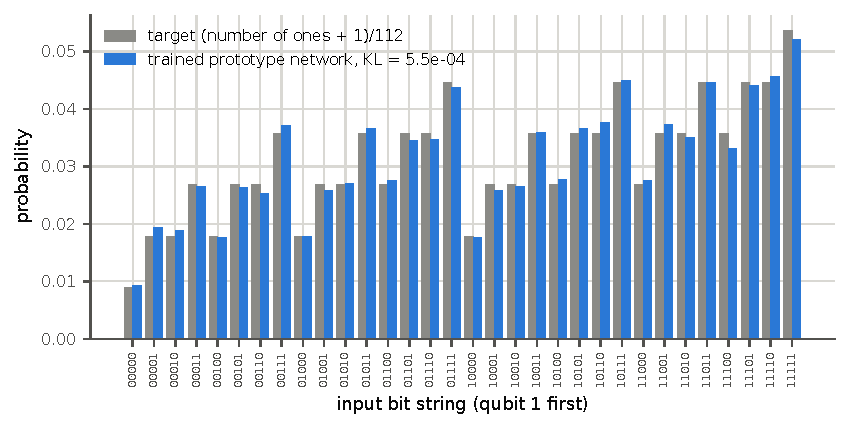
\includegraphics[width=\columnwidth]{fig_bitcount_histograms}
\caption{Target histogram (grey) and the trained prototype network's model distribution
(blue) over the 32 input strings; $\KL=5.5\times10^{-4}$.  Run
\run{bitcount\_noise/20260820T145335Z}, seed 1.}
\label{fig:agentic-histograms}
\end{figure}

\begin{figure}[tb]
\centering
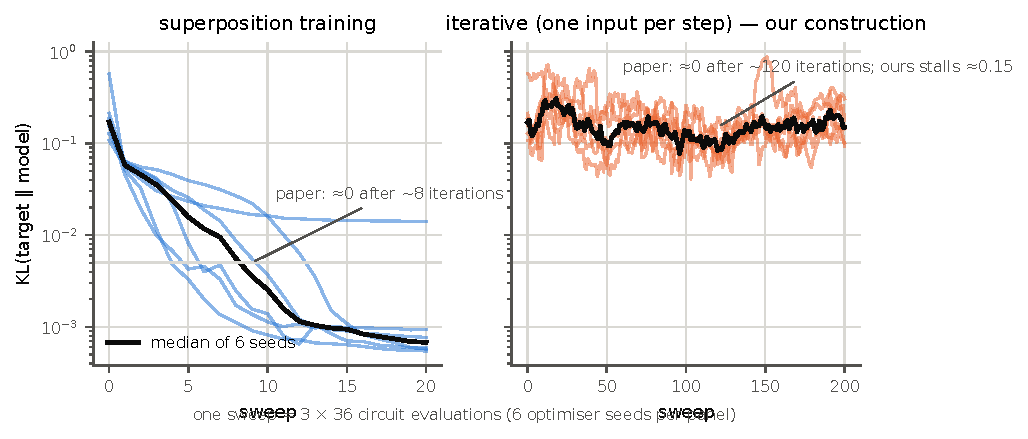
\includegraphics[width=\columnwidth]{fig_bitcount_convergence}
\caption{Left: superposition training, six optimiser seeds and their median.  Right: the
reimplementation's construction of the iterative baseline, which does not reach the
published curve.  Run \run{bitcount/20260820T135930Z}.}
\label{fig:agentic-convergence}
\end{figure}

\subsection{Iris}
\label{app:iris}

How the label enters the amplitude is not stated.  The published bar heights --- $1/86$, $4/86$,
$9/86$ on the training set and $1/154$, $4/154$, $9/154$ on the test set, two independent
integer normalisations --- fix the weight of class $\ell$ as $\propto(\ell+1)^2$: the amplitude
carries $\ell+1$ and the histogram its square, and no other exponent produces both
normalisations.  The split is not stated either; a stratified one-third training split
(50 flowers) is used.  Each feature is quantised into three $k$-means clusters, giving a 12-bit
one-hot code per flower, and the training set is loaded as one superposition over its distinct
codes; the network has 12 inputs, 4 hidden neurons and one output (17 qubits), against a
classic-neuron network of the same size, with labels predicted by rounding each code's read-out
weight.

In \cref{fig:agentic-iris-losses} the classic network drives its training loss to $10^{-5}$
within a few sweeps while its test loss bottoms out early and stays at $0.03$--$0.04$ --- it
memorises --- whereas the prototype network descends more slowly on both and its test loss is
still falling at sweep~40.  Prototype test accuracy is $95\,\%$, $91\,\%$ and $98\,\%$ on the
three splits against the published $\approx98\,\%$; the encoding caps accuracy at $97\,\%$,
$99\,\%$ and $99\,\%$, since two flowers of different species can share a 12-bit code.  The
t-SNE picture of \cref{fig:tsne} does not reproduce: in this embedding both weight sets cluster
away from the data, and what was plotted is not recoverable from the text.

\paragraph{On the split.}
The published histograms show 15 non-empty bars for the training set and 30 for the test set.
The 50-flower training splits used here give 14, 12 and 14 distinct codes, close to 15, but the
100-flower test splits give only 20, 20 and 18, not 30: three clusters per feature do not
spread 100 flowers over 30 codes on any split tried.  The figure supports the \emph{direction}
of the split, not its ratio, which remains an assumption.  An earlier draft claimed the bar
counts justified the ratio; an independent review caught the over-reading and the justification
was withdrawn.

\begin{figure}[tb]
\centering
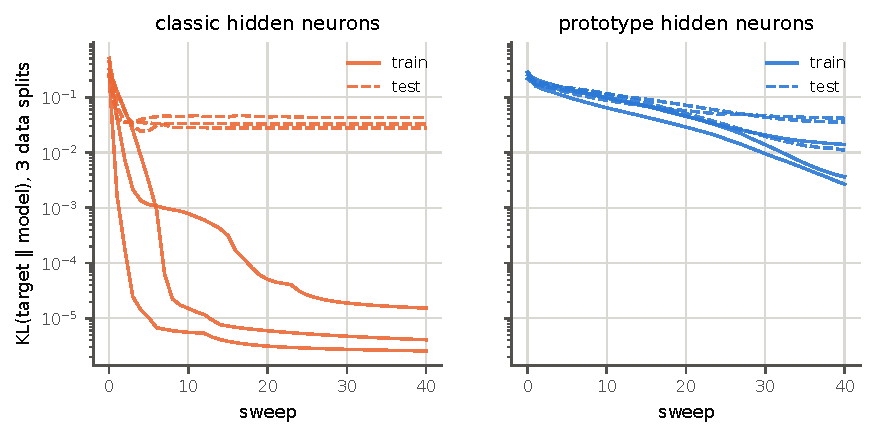
\includegraphics[width=\columnwidth]{fig_iris_losses}
\caption{Training (solid) and test (dashed) loss per sweep on three data splits, classic
against prototype network.  Runs \run{iris/20260820T144849Z}, \run{...T145454Z},
\run{...T145455Z}.}
\label{fig:agentic-iris-losses}
\end{figure}

\subsection{Flappy Bird}
\label{app:flappy}

The submission gives no reward, no training protocol and no game constants, so a
deterministic, window-free clone was built.  Its physics are a choice: the classic constants
(impulse $-9$, gap 100, spacing 144) are provably unplayable by a memoryless two-feature policy
--- one flap overshoots by 40.5\,px against a 38\,px budget --- so impulse $-7$, gap 120,
spacing 180 are used.  Height and the centre of the next gap enter two input qubits by
\cref{eq:agentic-encoding}; four prototype hidden neurons and one classic output flap when
$\Pout>\tfrac12$, 17 angles in all.  Training minimises the negative episode return (0.01 per
frame, 1 per pipe) plus a tracking term $|{\rm height}-{\rm gap}|$ supplying a slope where
every policy dies within 30 frames; 300 random vectors are scored on short episodes and the
best seeds 25 sweeps on five 1500-frame episodes.

The trained network passes 110 pipes in 5\,000 frames --- the cap, a perfect game --- on
all 20 held-out game seeds, for all 8 optimiser seeds tried, in about three minutes of training
(run \run{flappy/20260820T143753Z}); \cref{fig:agentic-flappy-policy} shows the learned
boundary.

\begin{figure}[tb]
\centering
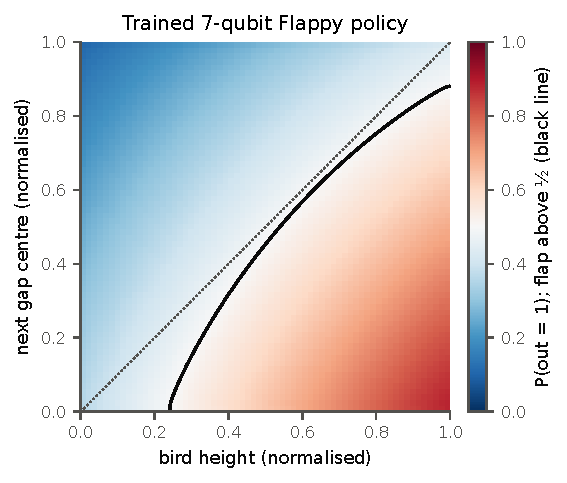
\includegraphics[width=0.85\columnwidth]{fig_flappy_policy}
\caption{The trained controller's activation $\Pout$ over the two observations; the black
line is the decision boundary $\Pout=\tfrac12$ (flap to its right), the dotted diagonal is
``bird at gap height''.  Run \run{flappy/20260820T143753Z}.}
\label{fig:agentic-flappy-policy}
\end{figure}

\subsection{ECG denoising}
\label{app:ecg}

Five consecutive noisy samples enter five input qubits; one to three prototype hidden neurons
and one output predict the clean centre sample as $\Pout$.  The recording is not identified;
the published trace is a smooth two-beat signal of 1\,800 samples in $[0,1]$ with additive
noise of standard deviation $\approx0.03$.  A synthetic ECG of McSharry form was generated to
match it, Gaussian noise of $\sigma=0.02$ added (noisy input $32.0$~dB), the first half used
for training and the second for test, and the experiment repeated on PhysioNet MIT-BIH
record~100~\cite{moody2001mitbih}.

PSNR is $37.4$, $38.0$ and $38.1$~dB for one, two and three prototype neurons against the
published $32.9$, $40.00$ and $40.04$: within about $2$~dB at two and three neurons, and $4$~dB
\emph{above} the published value at one neuron (\cref{fig:agentic-ecg-trace}).  The prototype
network beats the classic one at one and two neurons and on every SSIM; the classic one wins at
three.  The numbers cannot match exactly because the signal is not the authors' own.  The
alternative encoding $\theta=\pi s$ costs $0.6$--$7$~dB here, independent evidence for
\cref{eq:agentic-encoding}.  On MIT-BIH record~100 (run \run{ecg/20260820T165912}) the same
networks reach $36$--$38$~dB.

\begin{figure}[tb]
\centering
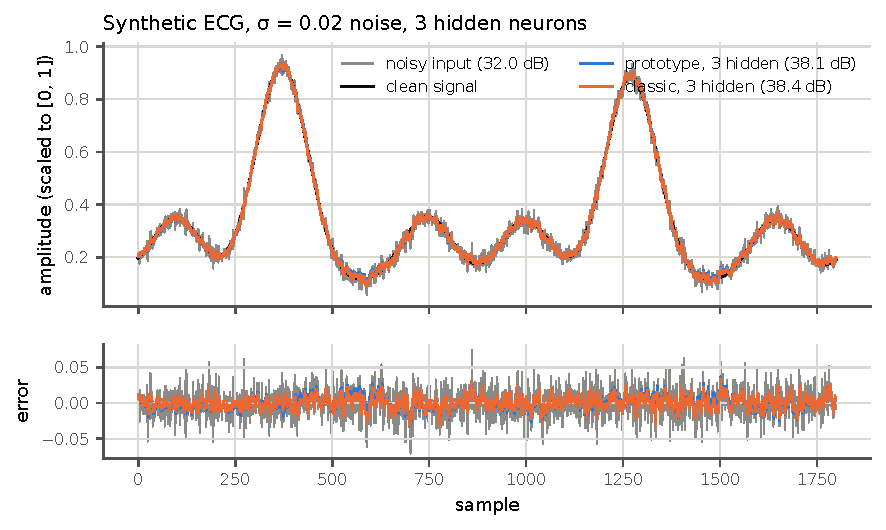
\includegraphics[width=\columnwidth]{fig_ecg_trace}
\caption{Noisy input, clean signal and the two three-neuron networks' outputs (top); their
errors (bottom).  Run \run{ecg/20260820T162014}.}
\label{fig:agentic-ecg-trace}
\end{figure}


\section{The experiments under calibrated noise}
\label{app:noise}

\subsection{Seven machines as noise models}
\label{app:devices}

Each vendor's published gate errors, gate durations, $T_1$, $T_2$, readout error and
connectivity were collected into a device file whose every field carries its source URL,
retrieval date (20 August 2026) and a verbatim quotation (\cref{app:provenance});
\cref{tab:agentic-devices} summarises them.  Three caveats govern everything that follows.
\emph{Quantinuum publishes no gate durations and no $T_1$/$T_2$}: its idle error is charged
from its published memory error per depth-1 circuit time ($2.0\times10^{-4}$ for H2-1,
$2.2\times10^{-4}$ for H1-1), and its simulated noise carries no idle error.  \emph{Rigetti
publishes only a two-qubit error} for Ankaa-3, its $99.5\,\%$ headline being for a different
gate than the universal one needed here, so every Rigetti number is an upper bound.
\emph{IQM's $T_1$/$T_2$ are a third-party snapshot}, and its $T_2$ without echo is $8.5\,\mu$s
against the $21\,\mu$s echo value used.  Where a vendor publishes nothing, the channel is
modelled as error-free and flagged, not invented.

\begin{table*}[t]
\caption{The seven device presets (medians where the vendor publishes per-qubit tables).
Two-qubit error $\varepsilon_2$, one-qubit error $\varepsilon_1$, readout error (mean of
$p_{01}$, $p_{10}$), coherence times, two-qubit gate time.  ``---'' = not published.}
\label{tab:agentic-devices}
\begin{tabular}{@{}l l S[table-format=1.2e-1] S[table-format=1.1e-1] S[table-format=1.1e-1] l l S[table-format=6.0]@{}}
\toprule
Machine & Connectivity & {$\varepsilon_2$} & {$\varepsilon_1$} & {readout} & $T_1$ & $T_2$ & {2q gate (ns)} \\
\midrule
Quantinuum H1-1 & all-to-all & 9.7e-4 & 1.8e-5 & 2.3e-3 & --- & --- & {---} \\
Quantinuum H2-1 & all-to-all & 1.1e-3 & 1.9e-5 & 1.0e-3 & --- & --- & {---} \\
IonQ Forte & all-to-all & 4.0e-3 & 2.0e-4 & 5.0e-3 & 55\,s & 1\,s & 950000 \\
Google Willow & square & 4.1e-3 & 5.3e-4 & 8.0e-3 & $68\,\mu$s & $89\,\mu$s & 42 \\
IBM Fez (Heron r2) & heavy-hex & 3.9e-3 & 2.3e-4 & 7.7e-3 & $145\,\mu$s & $88\,\mu$s & 84 \\
IQM Garnet & square & 4.9e-3 & 8.0e-4 & 3.0e-2 & $27\,\mu$s & $21\,\mu$s & 30 \\
Rigetti Ankaa-3 & square & 1.0e-2 & {---} & {---} & --- & --- & 72 \\
\bottomrule
\end{tabular}
\end{table*}

\subsection{Bit-count}
\label{app:noise-bitcount}

The trained 11-qubit networks were evaluated exactly, as density matrices on the GPU, under
each preset (run \run{bitcount\_noise/20260820T145335Z};
\cref{fig:agentic-noise-devices}).  The model distribution moves by $\TV=0.005$ (Quantinuum
H2-1) to $0.039$ (IQM Garnet), and the KL to the target rises from $5.5\times10^{-4}$ to
$7\times10^{-4}$ on H2-1 and to $6\times10^{-3}$ on Garnet.  The prototype network is better
under every preset, but the displacement \emph{caused} by the noise,
$\KL(\text{clean}\,\|\,\text{noisy})$, is the same for both (median $0.0021$ against $0.0022$):
they have identical two-qubit gate counts, so the prototype's advantage under noise is
inherited from its better noiseless fit, not from robustness of the neuron type.  Scaling IBM
Fez's noise by $s$ gives $\KL\propto s^{1.7}$ and $\TV\propto s^{0.95}$.

Training \emph{under} the noise works, on a 7-qubit version (3 inputs, 3 hidden; the 11-qubit
grid would have cost 13 hours and was not run): it recovers the noisy KL by a median factor of
$158$ (prototype) and $361$ (classic), \cref{fig:agentic-noise-aware}.  But the recovered
parameters are \emph{worse} on a noiseless simulator --- the optimiser folds the channel into
the angles instead of finding noise-robust ones.

\begin{figure}[tb]
\centering
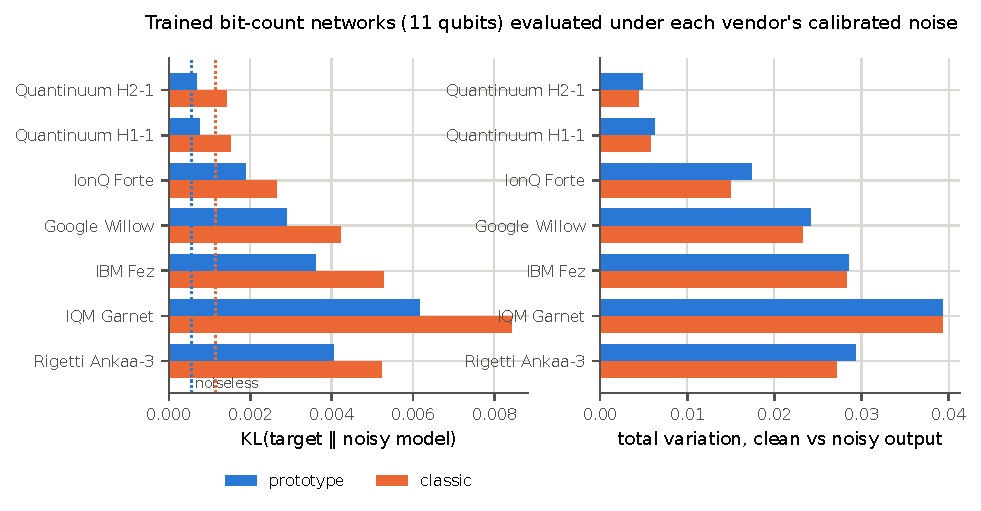
\includegraphics[width=\columnwidth]{fig_bitcount_noise_devices}
\caption{The trained bit-count networks under each machine's noise model.  Left: KL to the
target, noiseless values dotted.  Right: how far the output distribution moved.  Rigetti's
row models only its two-qubit error.  Run \run{bitcount\_noise/20260820T145335Z}.}
\label{fig:agentic-noise-devices}
\end{figure}

\begin{figure}[tb]
\centering
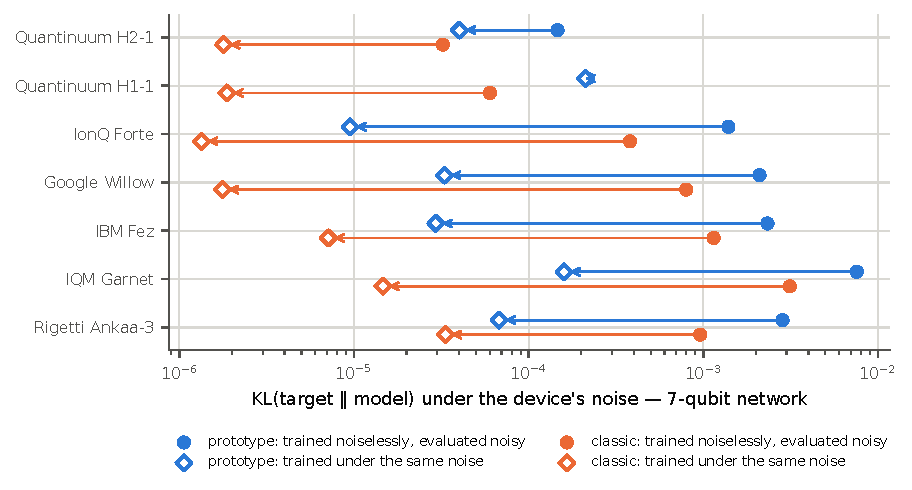
\includegraphics[width=\columnwidth]{fig_bitcount_noise_aware}
\caption{Noise-aware training of the 7-qubit bit-count network: KL under each machine's noise
for parameters trained noiselessly (filled) and with the same noise model in the loop (open),
median of three seeds.  Same run.}
\label{fig:agentic-noise-aware}
\end{figure}

\subsection{Flappy Bird}
\label{app:noise-flappy}

For a thresholded activation what matters is not how far $\Pout$ moves but whether it crosses
$\tfrac12$.  Evaluated exactly under every preset on its $65\times65$ decision grid and played
for 20 held-out games (run \run{flappy\_noise/20260820T154249Z};
\cref{fig:agentic-flappy-noise}), the controller \emph{still plays perfectly on all seven
machines}: only $1.5$--$4\,\%$ of visited frames are decided differently, because the noise
contracts every activation toward $\tfrac12$ by about the same amount (mean
$|\Delta P|=0.002$--$0.018$) and so rarely changes the ordering.  There is a factor of two of
headroom: Fez's noise scaled by $2$ leaves $60\,\%$ of games perfect, by $4$ none.

Shot noise is a different matter (\cref{fig:agentic-flappy-shot-noise}).  Re-deciding every
frame from $N$ measurements, the controller wins no game at $N=1\,000$, $90\,\%$ at $4\,000$
and all at $10\,000$ noiselessly; on Fez's model only $55\,\%$ at $4\,000$.  The cause is the
margin distribution over played frames: median $\delta=0.019$, tenth percentile $0.004$, first
percentile $0.0002$; the measured flip rate agrees with the average of $\Phi(-2\delta\sqrt N)$
over it to $3\,\%$.  A deterministic shift of the boundary is tolerated far past a stochastic
one --- Fez at scale $2$ decides $20\,\%$ of frames differently and still wins $60\,\%$ of
games, while $1\,000$ shots decide only $8.5\,\%$ differently and win none ---.  Fine-tuning under Fez's noise for five sweeps changes nothing: the training
episodes all survive already, so the objective has no slope.

\begin{figure}[tb]
\centering
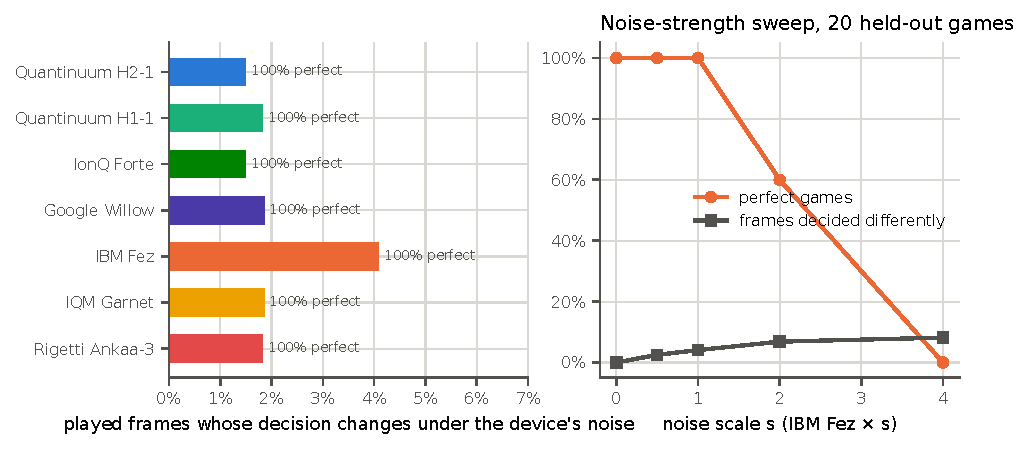
\includegraphics[width=\columnwidth]{fig_flappy_noise}
\caption{Flappy under gate noise.  Left: fraction of played frames whose decision changes
under each machine's model; every machine still yields $100\,\%$ perfect games.  Right: IBM
Fez's noise scaled by $s$.  Run \run{flappy\_noise/20260820T154249Z}.}
\label{fig:agentic-flappy-noise}
\end{figure}

\begin{figure}[tb]
\centering
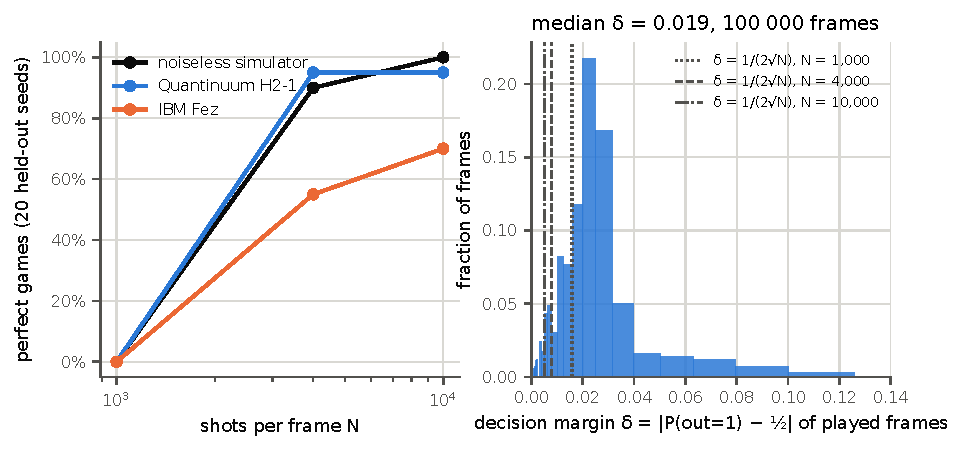
\includegraphics[width=\columnwidth]{fig_flappy_shot_noise}
\caption{Flappy under shot noise.  Left: perfect games when every frame is decided from $N$
shots.  Right: distribution of the decision margin $\delta$ over the $100\,000$ frames the
noiseless controller plays; vertical lines mark the margin that $N$ shots can just resolve.
Same run.}
\label{fig:agentic-flappy-shot-noise}
\end{figure}

\subsection{ECG and Iris, reduced run}
\label{app:noise-ecg-iris}

These two grids were run in a \emph{reduced} configuration only (run
\run{ecg\_iris\_noise/20260820T155618Z}): ECG on 8 test windows instead of 898 and two presets
instead of seven; Iris with 16 Monte-Carlo trajectories per evaluation instead of 2\,000
(per-outcome standard error $\approx12\,\%$), two presets, and perfect preparation of the
dataset state assumed.  The full grids cost 4--6 CPU-hours (ECG) and 8 hours (Iris), outside
the budget.  The results (\cref{fig:agentic-ecg-iris-noise}) are indicative only: ECG loses
$-0.1$ to $+0.4$~dB under Quantinuum H2-1 and $1.6$--$2.7$~dB (classic) under IBM Fez, while
the prototype cells \emph{gain} up to $3.8$~dB under Fez on eight windows --- a small-sample
artefact, not a finding.  Iris keeps its $95\,\%$ accuracy under H2-1 and loses it under Fez
($64\pm44\,\%$ over two trajectory seeds) for the prototype network, whose read-out is a
conditional distribution over 4\,096 input strings and is therefore directly exposed to
probability leaking out of the 20-code support.  One noisy sweep of ECG fine-tuning gains
$2.7$~dB under Fez and $3.7$~dB noiselessly: it finishes the clean optimisation, it does not
fold the channel in.

\begin{figure}[tb]
\centering
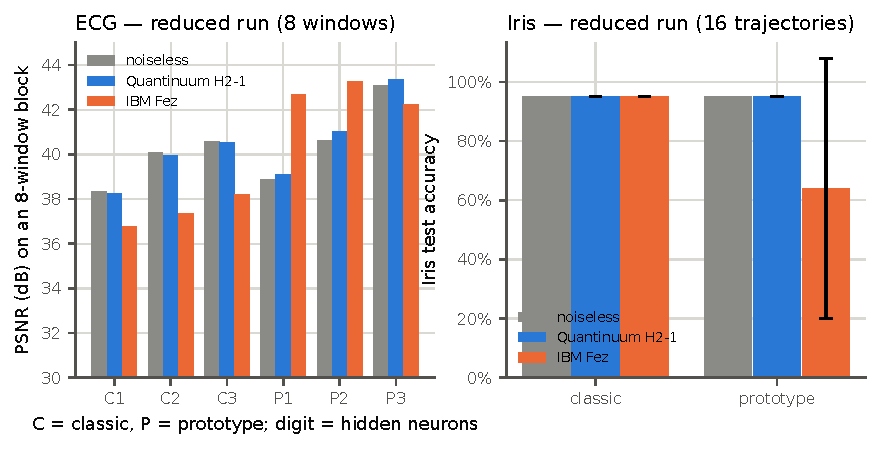
\includegraphics[width=\columnwidth]{fig_ecg_iris_noise}
\caption{Reduced-configuration noise runs, quoted for the record.  Left: ECG PSNR on an
8-window block.  Right: Iris test accuracy from 16 trajectories, error bars over two
trajectory seeds.  Run \run{ecg\_iris\_noise/20260820T155618Z}.}
\label{fig:agentic-ecg-iris-noise}
\end{figure}


\section{What it takes to run this on a real machine}
\label{app:hardware}

All numbers here are printed by one script into \run{hardware-plan/20260821T084554Z} (file
\code{numbers.md}); it joins every calibration number to its provenance entry and refuses to
run if one is missing.

\subsection{Compilation}
\label{app:compile}

Every prototype neuron touches every input, so the two-qubit gates form a complete bipartite
graph between inputs and hidden qubits --- the worst case for a lattice.  On an all-to-all
machine each controlled rotation costs exactly two native two-qubit gates: 24 for Flappy, 60
for bit-count.  On a lattice the compiler must insert SWAPs at three native gates each; with a
greedy router the bit-count circuit needs 327 native two-qubit gates on IBM's heavy-hex lattice
and 207 on a square lattice, $82\,\%$ and $71\,\%$ of them SWAP-borne
(\cref{fig:agentic-entanglers}).  IBM's own compiler needs 97 at optimisation level~2,
$3.4\times$ fewer, so this router is a device-independent comparison instrument and not what
one would submit.  The Flappy circuit is $12.9\,\mu$s long on Fez ($1.56\,\mu$s of it readout)
and 17.9\,ms on IonQ Forte, whose gates take a millisecond.

\begin{figure}[tb]
\centering
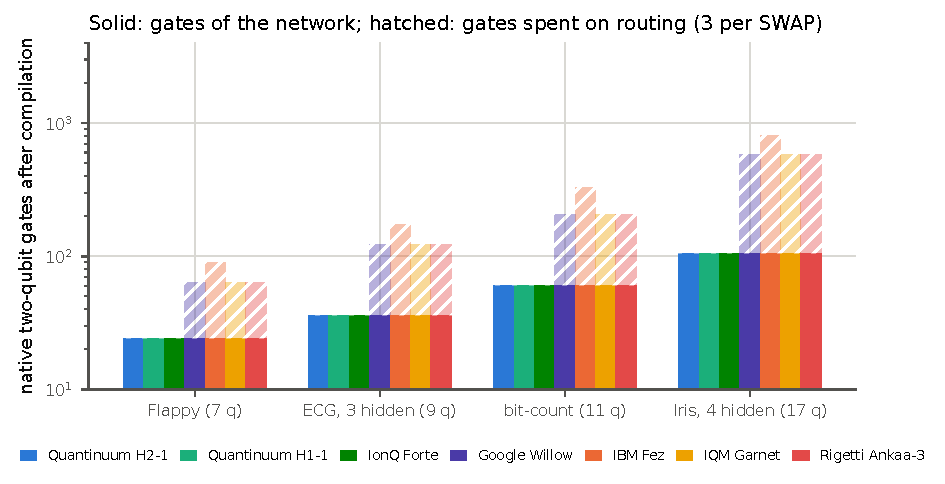
\includegraphics[width=\columnwidth]{fig_hardware_entanglers}
\caption{Native two-qubit gates after compiling each network for each machine (greedy router,
log scale).  All-to-all machines need only the network's own gates; the lattices spend most of
their budget on routing.  Run \run{hardware-plan/20260821T084554Z}.}
\label{fig:agentic-entanglers}
\end{figure}

\subsection{Expected fidelity}
\label{app:fidelity}

\Cref{fig:agentic-fidelity} stacks the four factors of \cref{eq:agentic-fidelity} for the two
smallest circuits, with the exactly simulated total-variation distance between the compiled
circuit run clean and run under noise beside each bar.  Flappy at 7 qubits is a high-fidelity
circuit on trapped ions ($F\approx0.92$ on H2-1, $0.83$ on Forte), marginal on Willow and Fez
($0.63$; $0.46$ with the greedy router, $0.75$ with IBM's compiler) and poor on Garnet
($0.24$).  Bit-count at 11 qubits is feasible on the H-series ($0.81$) and Forte ($0.64$),
usable with IBM's compiler on Fez ($0.48$) and dead on Garnet ($0.008$), whose routed circuit
lasts $86\,\%$ of its $T_2$.  Idling is charged only over each qubit's schedule gaps, since
relaxation during a gate is already inside the vendor's gate error; charging the whole circuit
duration on every qubit is $10$--$15$ points more pessimistic on the superconducting machines
and is printed beside it in the run directory.

Two cautions.  The simulated distances of the \emph{compiled} circuits ($0.03$ on the H-series,
$0.16$ on Forte, $0.43$ on Fez) are $5$--$15\times$ larger than for the uncompiled circuits of
\cref{app:noise-bitcount}.  And vendors' two-qubit errors are measured in isolation --- IBM's
own layered benchmark for Fez is $1.7\times$ worse than its isolated gate error --- so the
lattice numbers are optimistic.

\begin{figure*}[t]
\centering
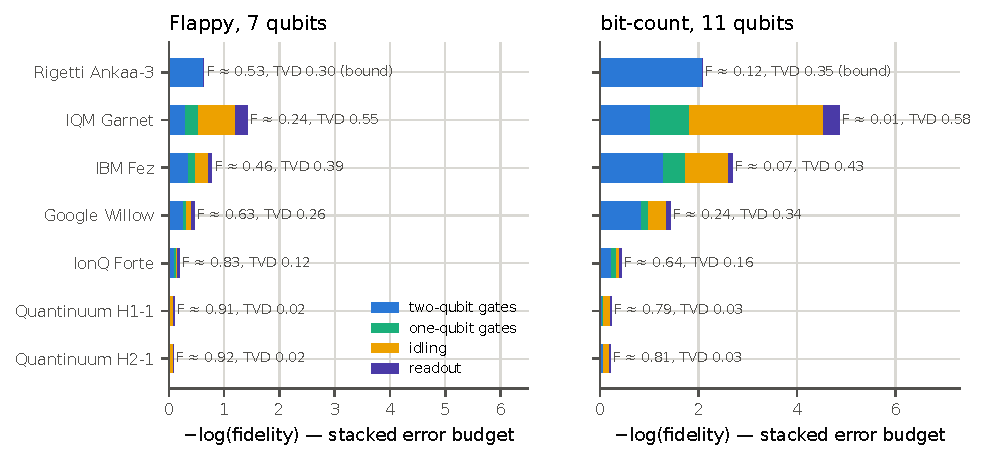
\includegraphics[width=0.92\textwidth]{fig_hardware_fidelity}
\caption{Error budget per machine for the Flappy (left) and bit-count (right) circuits: the
stacked bars are $-\log$ of each factor of \cref{eq:agentic-fidelity}, so their total is
$-\log F$; labels give $F$ and the simulated total-variation distance of the compiled circuit.
Quantinuum's idle term comes from its published memory error; Rigetti's is a bound from its
two-qubit error only.}
\label{fig:agentic-fidelity}
\end{figure*}

\subsection{Shots, time and money}
\label{app:cost}

An activation to $\pm0.005$ needs $10\,000$ shots.  The 32-bin bit-count histogram is estimated
from the shots in which the output fired ($\Pout=0.487$ of them), so the plug-in KL is biased
upward by $(K-1)/(2\cdot0.487\cdot N)=31.8/N$ with $K=32$; reaching the trained model's
$5.5\times10^{-4}$ needs $58\,000$ shots, rounded to a $64\,000$-shot job.  The ECG PSNR is
capped by shot noise at $10\log_{10}(4N)$, so $2\,500$ shots per sample cap it at exactly
$40$~dB --- the published Table~I value --- and a $1\,800$-sample trace at $25\,000$ shots is
$4.5\times10^7$ shots: ECG is a simulator experiment.  Machine time per job is milliseconds to
two seconds on the superconducting machines, where the per-job overhead dominates, but $72$\,s
(Flappy) and 32 minutes (bit-count) on IonQ Forte, where circuit time does.

Prices retrieved 20 August 2026 are in \cref{tab:agentic-cost}.  Training on hardware is out of
the question: $2\,160$ evaluations at $64\,000$ shots are $1.4\times10^8$ shots, 48 days of
Forte time or \$11\,M.  Fine-tuning the six output angles (90 evaluations at $4\,000$ shots) is
$1.8$ hours on Forte, about 45 minutes on Fez.  Live play is equally out: $1\,500$ frames
$\times$ $4\,000$ shots $\times$ $17.9$\,ms is 30 hours per episode on Forte.  The falsifiable
hardware observable is instead the activation map of \cref{fig:agentic-flappy-policy} on a grid
of observations, 16 jobs.

\begin{table*}[t]
\caption{Cost per job (file \code{numbers.md}, section ``cost'').  IBM: \$1.60 per QPU second
plus a 30\,s per-job overhead, both assumptions (\cref{app:assumptions}); Quantinuum: the
vendor's credit formula converted at the Azure plan rate; Braket: published per-shot prices.}
\label{tab:agentic-cost}
\begin{tabularx}{\textwidth}{@{}l X l l@{}}
\toprule
Machine & Price model & Flappy, 4\,000 shots & bit-count, 64\,000 shots \\
\midrule
IBM Fez & \$1.60/s; 52\,ms resp.\ 1.8\,s of QPU & \$0.08 (\$48 with overhead) & \$2.85 (\$51) \\
IBM Open plan & 10 min per 28 days, free & \$0 & \$0 \\
Quantinuum H1/H2 & credits $=5+(N_1+10N_2+5N_m)C/5000$ & 323 credits $\approx$ \$4\,030 & 11\,920 credits $\approx$ \$149\,000 \\
IonQ Forte (Braket) & \$0.30 + \$0.08/shot & \$320 & \$5\,120 \\
IQM Garnet (Braket) & \$0.30 + \$0.00145/shot & \$6.10 & \$93 \\
\bottomrule
\end{tabularx}
\end{table*}

\subsection{Recommendation}
\label{app:recommendation}

Run the 7-qubit Flappy activation map first: on IBM's free plan to debug the pipeline (readout
calibration, then zero-noise extrapolation by gate folding, both validated offline against the
noise model), then on IonQ Forte for the confirmation (\$1\,300 for a $4\times4$ grid at
$1\,000$ shots), and on Quantinuum H2-1 for the headline number if an allocation exists.  The
bit-count histogram is feasible on the H-series and Forte as a \emph{shape} demonstration but
not as a KL comparison: device error puts the KL floor at $10^{-2}$--$10^{-1}$, two orders
above the simulated $5.5\times10^{-4}$.  Iris cannot be settled yet.  What these runs prepare
is a uniform superposition over the $12$--$14$ \emph{distinct} training codes, not over the 120
samples an earlier draft assumed; the sparse state-preparation construction of Gleinig and
Hoefler~\cite{gleinig2021sparse} has leading term $k\cdot n=144$--$168$ two-qubit gates, giving
$F\approx0.83$ on H2-1 and $\approx0.75$ with the network --- but its constant is unknown, and
the dense alternatives ($8\,168$ gates by Shende--Bullock--Markov synthesis, $\approx3\,925$ by
Plesch--Brukner) are hopeless.  An exact answer needs an actual sparse state-preparation
circuit, which the repository does not build.  For a live submission the code still lacks
credentials, the vendors' own routing, asynchronous job handles, and readout-unfolding and
gate-folding utilities.


\section{The shot-noise programme}
\label{app:shots}

What limits a hardware demonstration is the number of measurements, through two mechanisms: a
thresholded controller flips at a rate $\Phi(-2\delta\sqrt N)$, and a histogram loss estimated
from $N$ shots is biased upward by $(K-1)/(2\,\Pout\,N)$ while discarding the half of the shots
in which the output did not fire.  Six remedies were proposed and three implemented.  The
others --- a joint-distribution loss or amplitude amplification so that all shots are used,
bias-corrected KL estimators, and amplitude estimation --- are designed but not implemented;
the first is the natural next step, since the estimator bias is what now limits sampled
training.  All runs here are noiseless state-vector simulations plus sampling.

\subsection{Margin-aware training: negative}
\label{app:margin}

If every frame had $\delta\ge0.1$ instead of the median $0.019$, the shots per frame would fall
by $(0.1/0.019)^2\approx25\times$ at no noiseless cost.  A penalty
$w\times0.01\times\max(0,1-\delta/m)$ per played frame was added --- a fraction $w<1$ of the
$0.01$ reward for surviving that frame, so surviving always beats dying confidently --- and the
controller fine-tuned for 25 sweeps with $m=0.1$, $w\in\{0.25,0.5,1\}$ (run
\run{flappy\_shots/20260821T084601Z}).  An earlier attempt with a \emph{mean} hinge of weight
20, trained from scratch, collapsed to a policy that died in 30 frames with perfectly confident
decisions (run \run{flappy\_shots/20260821T075048Z}): any penalty that can outweigh the
per-frame reward selects for dying early.

The margin quantiles hardly move (\cref{fig:agentic-flappy-shots}, left; median
$0.019\to0.021$--$0.024$, tenth percentile $0.004\to0.006$).  All three fine-tuned controllers
still play perfectly on exact probabilities, but under shot noise they play \emph{worse} than
the original at $w\ge0.5$ ($50\,\%$ and $80\,\%$ perfect games at $10\,000$ shots against
$100\,\%$).  The near-boundary frames are those in which the bird hovers at the boundary, a
property of the game's dynamics and not of the surface's steepness, so penalising them moves
the boundary rather than steepening it --- and a 17-parameter network has no spare capacity to
steepen its surface anyway.

\subsection{Common random numbers}
\label{app:crn}

A slope from $N$ independent shots per probe with variance $\sigma^2$ has variance
$\sigma^2/2c^2$, at $c=0.2$ some $12.5\sigma^2$, which is why finite differences on a sampling
backend stall.  Feeding the same uniform random numbers to both probes gives only a
$1.3\times$ reduction, because a parameter change moves probability between distant bit strings
and shifts every later bin boundary.  What works is the \emph{maximal coupling}: sample the
first probe, then for the second keep each outcome $i$ with probability
$\min(1,p_{\mathrm{new}}(i)/p_{\mathrm{ref}}(i))$ and redraw otherwise from
$(p_{\mathrm{new}}-p_{\mathrm{ref}})_+$.  The second sample has exactly the right distribution
and only $N\cdot\TV(p_{\mathrm{new}},p_{\mathrm{ref}})$ shots change; since $\TV\propto c$, the
slope's variance is $O(1/(cN))$ rather than $O(1/(c^2N))$, a gain of order $1/c$.  Coupling
reduces the variance of the slope, not the bias of a non-linear loss.  On hardware the analogue
is to interleave the $\pm c$ circuits in one job so they share the same drift.

Measured on one slope of the bit-count loss at 400 shots per probe, the reduction is
$\times2$--$3$ at $c=0.2$--$0.4$ and $\times22$--$29$ at $c=0.025$--$0.05$, both estimates
unbiased for the exact slope.  Training the 11-qubit network on a sampling backend (run
\run{bitcount\_shots/20260821T084558Z}) gives, after 20 sweeps, an exact KL improving from
$0.080$ to $0.059$ at $N=1\,000$ shots per evaluation, from $0.050$ to $0.014$ at $4\,000$, and
at $16\,000$ the two are within the seed-to-seed spread ($0.029$ against $0.033$) --- all an
order of magnitude above the exact-probability result ($0.0009$).  The likely reason is the
loss itself: a plug-in KL of a 32-bin histogram from about $N/2$ usable shots, biased by
$31.8/N$, with the reached KL tracking one to three times that bias.  Three seeds, one of which
stalls at $0.014$ even on exact probabilities, cannot separate estimator from optimiser; a
bias-corrected or joint loss under paired initialisations is the test, and it has not been run.
The schedule used ($c_0=0.2$ decaying only to $0.15$ over 20 sweeps) also keeps the optimiser
where the reduction is smallest.

\subsection{Sequential decisions: positive}
\label{app:sprt}

A fixed budget wastes most of its shots: a frame with $\delta=0.3$ is decided correctly after a
dozen.  Wald's sequential probability ratio test~\cite{wald1945} between
$\Pout=\tfrac12\pm\delta_0$ draws shots in blocks, computes after $n$ shots with $k$ ones the
log-likelihood ratio $\Lambda=(2k-n)\log\frac{1+2\delta_0}{1-2\delta_0}$, and stops when
$\Lambda\ge\log\frac{1-\beta}{\alpha}$ (flap) or $\Lambda\le\log\frac{\beta}{1-\alpha}$ (do
not), up to a cap after which the majority decides.  Beyond $\delta_0$ its error probability is
at most about $\alpha$ ($=\beta=5\,\%$ here); nearer the boundary it is slow and unbounded.

On the same 20 held-out games (\cref{fig:agentic-flappy-shots}; \cref{tab:agentic-sprt}) the
rule with $\delta_0=0.01$ and cap $10\,000$ wins \emph{every} game at a mean of $2\,191$ shots
per frame, against the $10\,000$ a fixed budget needs for the same result --- $4.6\times$ fewer
--- and with $\delta_0=0.005$, cap $4\,000$ it matches the fixed $4\,000$-shot result
($85\,\%$) at $2\,916$.  Setting $\delta_0$ at the median margin ($0.02$) fails ($30\,\%$
perfect at $822$ shots): the frames that decide a game are the near-boundary ones, so the
indifference margin must sit below \emph{their} margins, the tenth percentile of
$0.004$--$0.006$.  The rule needs no change to the network and no retraining.

\begin{figure*}[t]
\centering
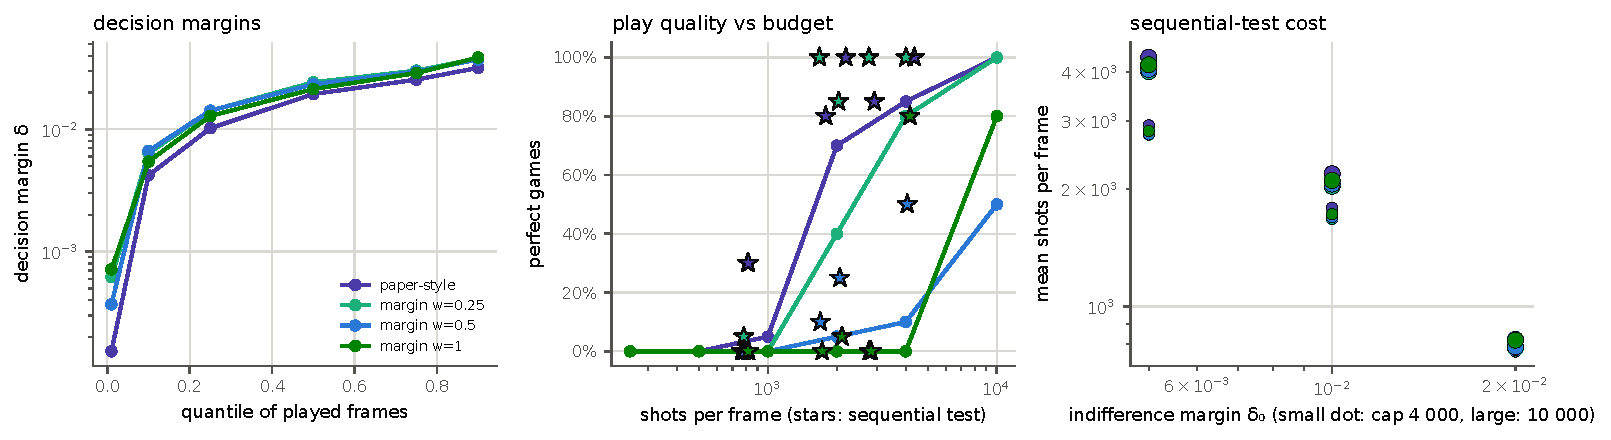
\includegraphics[width=\textwidth]{fig_flappy_shots_programme}
\caption{Flappy under shot noise, remedies 1 and 3.  Left: decision-margin quantiles of the
frames played by the original and the three margin-aware controllers.  Middle: perfect games
against shots per frame for a fixed budget (lines) and for the sequential test (stars, plotted
at the mean number of shots it actually spent).  Right: mean shots per frame of the sequential
test against its indifference margin $\delta_0$.  Run
\run{flappy\_shots/20260821T084601Z}.}
\label{fig:agentic-flappy-shots}
\end{figure*}

\begin{table*}[t]
\caption{Flappy, original controller, 20 held-out games: fixed shot budgets against the
sequential test ($\alpha=\beta=0.05$, blocks of 20 shots).  ``Flips'' are frames decided
differently from the exact rule.  Run \run{flappy\_shots/20260821T084601Z}.}
\label{tab:agentic-sprt}
\begin{tabular}{@{}l S[table-format=3.0] S[table-format=3.0] S[table-format=2.2] S[table-format=5.0]@{}}
\toprule
Decision rule & {perfect games (\%)} & {median pipes} & {flips (\%)} & {mean shots/frame} \\
\midrule
fixed $N = 1\,000$ & 5 & 23 & 8.36 & 1000 \\
fixed $N = 2\,000$ & 70 & 110 & 7.40 & 2000 \\
fixed $N = 4\,000$ & 85 & 110 & 6.09 & 4000 \\
fixed $N = 10\,000$ & 100 & 110 & 4.47 & 10000 \\
sequential, $\delta_0 = 0.02$, cap $10\,000$ & 30 & 88 & 7.19 & 822 \\
sequential, $\delta_0 = 0.01$, cap $4\,000$ & 80 & 110 & 6.12 & 1790 \\
sequential, $\delta_0 = 0.005$, cap $4\,000$ & 85 & 110 & 5.98 & 2916 \\
sequential, $\delta_0 = 0.01$, cap $10\,000$ & 100 & 110 & 5.06 & 2191 \\
sequential, $\delta_0 = 0.005$, cap $10\,000$ & 100 & 110 & 4.50 & 4358 \\
\bottomrule
\end{tabular}
\end{table*}


\section{What the reproduction learned}
\label{app:learnings}

\begin{enumerate}
\item \textbf{The central claims reproduce.}  Activation surface, bit-count histogram and
convergence, Iris overfitting contrast, perfect Flappy play on a clone, ECG denoising within
2~dB on a different signal.  What does not: the iterative baseline of \cref{fig:OptConv} (this
construction stalls at $\KL\approx0.15$) and the weight picture of \cref{fig:tsne}; both are
under-specified in the text.

\item \textbf{Reading figures is part of reproduction.}  The bit-count target
$(\text{ones}+1)/112$, the Iris label weighting $(\ell+1)^2$ and the angle encoding
$\theta=2\arcsin\sqrt s$ were all read off figures and then confirmed to the figure's
precision.  Where a figure was over-read --- the Iris split ratio --- an independent review
caught it and the justification was withdrawn (\cref{app:iris}).

\item \textbf{The prototype network's advantage under noise is inherited, not intrinsic.}  Both
networks have the same two-qubit gate count and the noise displaces both equally; the prototype
wins under noise because it fits better without it.

\item \textbf{Gate noise at published levels is not the obstacle; shots are.}  Every
7--11-qubit network survives every vendor's calibrated model with a qualitatively intact
result, while the Flappy controller needs $10^4$ shots per frame at a fixed budget and the
bit-count loss is biased by $31.8/N$.  The one remedy that pays now is the sequential rule
($4.6\times$ fewer shots, no retraining); margin-aware training does not work for a
17-parameter network; common random numbers reduce the optimiser's noise by $1/c$ but leave the
estimator's bias, the likely and as yet untested limit of sampled training.

\item \textbf{Compiled circuits are $5$--$15\times$ more noise-sensitive than logical ones.}
Two native gates per controlled rotation, resynthesised single-qubit gates and lattice routing
all cost; a complete-bipartite network is the worst case for a lattice, so the vendor's own
compiler must be used for any superconducting submission.  Trapped ions are the natural home of
this architecture, at the price of circuit time.

\item \textbf{An optimiser that keeps a stale incumbent turns a harmless change into a negative
result.}  The ``rotating episodes break training'' finding was an artefact of comparing losses
measured on different episode batches, because the optimiser kept its incumbent's loss from the
previous batch; re-scoring the incumbent on each batch restores $25/25$ perfect games (runs
\run{flappy/batch0}, \run{flappy/batch5}).  Any non-stationary objective needs this.

\item \textbf{Penalties must be priced in the currency of the reward.}  A margin hinge able to
outweigh the per-frame survival reward produced a confidently dead controller; the per-frame
form, kept below that reward, does not.

\item \textbf{Provenance has to be mechanical.}  The first hardware plan contained a dozen wrong
numbers: a state-preparation gate count off by a factor of two, a reversed inequality, costs
computed by hand.  The fix was a script that emits every number and refuses to run if any
calibration input lacks a source; this appendix quotes only that script.
\end{enumerate}


\section{Choices the submission leaves open}
\label{app:assumptions}

Each entry is marked \code{[ASSUMPTION]} where it enters the code.

\begin{description}
\item[Optimiser schedule.]  $a_n=a_0/(n+1)^{0.602}$, $c_n=c_0/(n+1)^{0.101}$, geometric
cooling; one iteration is a coordinate sweep.  Bit-count: $a_0=20$, $c_0=0.2$, $T_0=0.02$,
cooling $0.7$, 20 sweeps.  Flappy: $a_0=0.4$, $c_0=0.25$, $T_0=0.05$, cooling $0.9$, 25 sweeps
after 300 random restarts.  Iris: $a_0=2$, decay exponent $0.3$, $c_0=0.1$, 40 sweeps.  ECG:
100 sweeps with restarts.
\item[Iterative baseline.]  One optimiser sweep on the squared error of one random input per
iteration.
\item[Angle encoding.]  $\theta=2\arcsin\sqrt s$, pinned by a printed angle in the companion
paper; $\theta=\pi s$ tested as an ablation.
\item[KL regularisation.]  Model probability floored at $10^{-12}$ inside the logarithm.
\item[Iris.]  Stratified one-third training split; flowers sharing a code are merged and their
labels averaged; the KL is normalised over all 4\,096 input strings, since restricting it to
the dataset's codes lets the network exploit interference between examples and reach a training
loss of $10^{-5}$ while reading out at chance; label weight $\propto(\ell+1)^2$; labels
predicted by nearest rounding of the read-out weight.
\item[Flappy.]  Clean-room clone: $288\times512$ screen, flap impulse $-7$, gap 120, pipe
spacing 180, gravity 1; reward 0.01 per frame plus 1 per pipe; tracking term
$|{\rm height}-{\rm gap}|$ with weight 1; 5 training episodes of 1\,500 frames, 20 held-out
seeds 5--24, 5\,000-frame cap (110 pipes); decisions cached on a $65\times65$ grid.
\item[ECG.]  Synthetic McSharry-form signal tuned to the published trace, and MIT-BIH
record 100; Gaussian noise $\sigma=0.02$; mirror-padded edges; first half train, second half
test; PSNR with $R$ the range of the clean signal; SSIM in a 7-sample sliding window.
\item[Noise model.]  Depolarising at the vendor's average gate error, relaxation during gates
and as-soon-as-possible idling, readout confusion; medians where vendors publish per-qubit
tables; no crosstalk, since no vendor publishes a usable number.  Quantinuum's idle error is
charged as $(1-m)^{n_{\rm qubits}\cdot{\rm depth}}$ from its memory error per depth-1 time;
IQM's and Rigetti's unpublished one-qubit gate durations are set to 40\,ns.
\item[Fidelity estimate.]  First-order product of per-gate survival probabilities; readout
factor $(1-(p_{01}+p_{10})/2)^n$.
\item[Costs.]  IBM \$1.60 per QPU second (2022 launch figure, corroborated by a secondary
\$96/min report) plus 30\,s per-job overhead; Quantinuum \$12.5 per credit (Azure Standard plan
divided by its allotment); Braket and Azure per-shot prices as retrieved on 20 August 2026;
Quantinuum's credit formula with $N_m=2\times$ qubits.
\item[State preparation.]  Dense counts $2^{n+1}-2n$ (Shende--Bullock--Markov) and
$\approx\tfrac{23}{24}2^n$ (Plesch--Brukner); sparse \emph{leading term} $k\cdot n$ of an
$O(kn)$ construction~\cite{gleinig2021sparse} with $k$ the $12$--$14$ distinct training codes
actually prepared, its constant unknown.
\item[Compilation.]  Lattice machines are compiled onto a synthetic heavy-hex or square patch
of the circuit's size with a greedy router; Google's and Rigetti's gate sets are rebased
through a generic fallback.  Idle relaxation is charged over each qubit's schedule gaps only.
\item[Shot-noise programme.]  Margin penalty $w\cdot0.01\cdot\max(0,1-\delta/m)$ per frame with
$m=0.1$; sequential test with $\alpha=\beta=0.05$ and blocks of 20 shots; common random numbers
by maximal coupling to the first probe of each coordinate.
\end{description}


\section{Provenance of the calibration data}
\label{app:provenance}

Every calibration number used in \cref{app:noise,app:hardware} is stored in a device file with
a provenance block per field: source URL, kind of source (vendor calibration page, vendor
paper, third-party snapshot), retrieval date and a verbatim quotation of the sentence or table
row the number was read from.  The hardware-plan script joins these blocks to every field it
reads and fails if any is missing; the full join, one row per device and field with quotations,
is the file \code{numbers.md} of run \run{hardware-plan/20260821T084554Z}.  In brief:

\begin{description}
\item[IBM Fez (Heron r2).]  One coherent calibration snapshot, backend version 1.2.8 of
2025-02-26, shipped as \code{props\_fez.json} in \code{qiskit-ibm-runtime}'s fake provider;
medians over 156 qubits and 352 directed CZ edges computed from that table.  The file records
the same chip drifting between CZ error $2.85\times10^{-3}$ (2024-07) and $3.90\times10^{-3}$
(2025-02).
\item[Quantinuum H1-1, H2-1.]  The vendor's performance-validation page: mean two-qubit and
one-qubit infidelities, SPAM error, ``Memory Error per Depth-1 Circuit Time''.  No gate
durations, no $T_1$/$T_2$.
\item[IonQ Forte.]  The vendor's published specification: average gate fidelities, gate
durations, $T_1=55$\,s, $T_2=1$\,s.
\item[Google Willow.]  Supplementary information of the Willow paper (\emph{Nature}, 2024):
gate errors, coherence times, cycle time.  Not publicly accessible; the preset exists for
simulation only.
\item[IQM Garnet.]  Vendor data for gate errors and readout; $T_1$ and $T_2$ (echo) from a
third-party calibration snapshot, two epochs recorded (December 2025, March 2026), with the
caveat that $T_2$ without echo is $\approx8.5\,\mu$s.
\item[Rigetti Ankaa-3.]  Only the two-qubit (iSWAP) error $10^{-2}$ is published for the
universal gate; the $99.5\,\%$ headline refers to the fSim gate.  No one-qubit error, no
readout error, no $T_1$ or $T_2$.
\end{description}

The per-field table is not reproduced here --- some sixty rows with quotations --- but it is
the ground truth every number in this appendix rests on, and it is one command away in the
repository at \repourl.


\end{document}
